%% Preamble %%
%% A minimal LaTeX preamble
%% Some packates are needed to implement
%% Asciidoc features


\documentclass[11pt]{amsbook}
\usepackage{geometry}                % See geometry.pdf to learn the layout options. There are lots.
\geometry{letterpaper}               % ... or a4paper or a5paper or ...
%\geometry{landscape}                % Activate for for rotated page geometry
%\usepackage[parfill]{parskip}       % Activate to begin paragraphs with an empty line rather than an indent

\usepackage{tcolorbox}
\usepackage{lipsum}

\usepackage{epstopdf}
\usepackage{color}
% \usepackage[usenames, dvipsnames]{color}
% \usepackage{alltt}


\usepackage{amssymb}
% \usepackage{amsmath}
\usepackage{amsthm}
\usepackage[version=3]{mhchem}


% Needed to properly typeset
% standard unicode characters:
%
\RequirePackage{fix-cm}
\usepackage{fontspec}
\usepackage[Latin,Greek]{ucharclasses}
%
% NOTE: you must also use xelatex
% as the typesetting engine


% \usepackage{fontspec}
% \usepackage{polyglossia}
% \setmainlanguage{en}

\usepackage{hyperref}
\hypersetup{
    colorlinks=true,
    linkcolor=blue,
    filecolor=magenta,
    urlcolor=cyan,
}

\usepackage{graphicx}
\usepackage{wrapfig}
\graphicspath{ {images/} }
\DeclareGraphicsExtensions{.png, .jpg, jpeg, .pdf}

%% \DeclareGraphicsRule{.tif}{png}{.png}{`convert #1 `dirname #1`/`basename #1 .tif`.png}
%% Asciidoc TeX Macros %%


% \pagecolor{black}
%%%%%%%%%%%%


% Needed for Asciidoc

\newcommand{\admonition}[2]{\textbf{#1}: {#2}}
\newcommand{\rolered}[1]{ \textcolor{red}{#1} }
\newcommand{\roleblue}[1]{ \textcolor{blue}{#1} }

\newtheorem{theorem}{Theorem}
\newtheorem{proposition}{Proposition}
\newtheorem{corollary}{Corollary}
\newtheorem{lemma}{Lemma}
\newtheorem{definition}{Definition}
\newtheorem{conjecture}{Conjecture}
\newtheorem{problem}{Problem}
\newtheorem{exercise}{Exercise}
\newtheorem{example}{Example}
\newtheorem{note}{Note}
\newtheorem{joke}{Joke}
\newtheorem{objection}{Objection}





%%%%%%%%%%%%%%%%%%%%%%%%%%%%%%%%%%%%%%%%%%%%%%%%%%%%%%%

%  Extended quote environment with author

\renewenvironment{quotation}
{   \leftskip 4em \begin{em} }
{\end{em}\par }

\def\signed#1{{\leavevmode\unskip\nobreak\hfil\penalty50\hskip2em
  \hbox{}\nobreak\hfil\raise-3pt\hbox{(#1)}%
  \parfillskip=0pt \finalhyphendemerits=0 \endgraf}}


\newsavebox\mybox

\newenvironment{aquote}[1]
  {\savebox\mybox{#1}\begin{quotation}}
  {\signed{\usebox\mybox}\end{quotation}}

\newenvironment{tquote}[1]
  {  {\bf #1} \begin{quotation} \\ }
  { \end{quotation} }

%% BOXES: http://tex.stackexchange.com/questions/83930/what-are-the-different-kinds-of-boxes-in-latex
%% ENVIRONMENTS: https://www.sharelatex.com/learn/Environments

\newenvironment{asciidocbox}
  {\leftskip6em\rightskip6em\par}
  {\par}

\newenvironment{titledasciidocbox}[1]
  {\leftskip6em\rightskip6em\par{\bf #1}\vskip-0.6em\par}
  {\par}



%%%%%%%%%%%%%%%%%%%%%%%%%%%%%%%%%%%%%%%%%%%%%%%%%%%%%%%%

%% http://texblog.org/tag/rightskip/


\newenvironment{preamble}
  {}
  {}

%% http://tex.stackexchange.com/questions/99809/box-or-sidebar-for-additional-text
%%
\newenvironment{sidebar}[1][r]
  {\wrapfigure{#1}{0.5\textwidth}\tcolorbox}
  {\endtcolorbox\endwrapfigure}


%%%%%%%%%%

\newenvironment{comment*}
  {\leftskip6em\rightskip6em\par}
  {\par}

  \newenvironment{remark*}
  {\leftskip6em\rightskip6em\par}
  {\par}


%% Dummy environment for testing:

\newenvironment{foo}
  {\bf Foo.\ }
  {}


\newenvironment{foo*}
  {\bf Foo.\ }
  {}


\newenvironment{click}
  {\bf Click.\ }
  {}

\newenvironment{click*}
  {\bf Click.\ }
  {}


\newenvironment{remark}
  {\bf Remark.\ }
  {}

\newenvironment{capsule}
  {\leftskip10em\par}
  {\par}

%%%%%%%%%%%%%%%%%%%%%%%%%%%%%%%%%%%%%%%%%%%%%%%%%%%%%

%% Style

\parindent0pt
\parskip8pt
%% User Macros %%
%% Front Matter %%

\title{Minor swing with Django}
\author{Cédric Declerfayt}
\date{}


%% Begin Document %%

\begin{document}
\maketitle
\tableofcontents
Nous n’allons pas vous mentir: il existe enormément de tutoriaux très bien réalisés sur "\emph{Comment réaliser une application Django}" et autres "\emph{Déployer votre code en 2 minutes}". Nous nous disions juste que ces tutoriaux restaient relativement haut-niveaux et se limitaient à un contexte donné.


L’idée du texte ci-dessous est de jeter les bases d’un bon développement, en survolant l’ensemble des outils permettant de suivre des lignes directrices reconnues, de maintenir une bonne qualité de code au travers des différentes étapes (du développement au déploiement) et de s’assurer du maintient correct de la base de code, en permettant à n’importe qui de reprendre le développement.


Ces idées ne s’appliquent pas uniquement à Django et à son cadre de travail, ni même au langage Python. Juste que ces deux sujets sont de bons candidats et que le cadre de travail est bien défini et suffisamment flexible.


Django se présente comme un "\href{https://www.djangoproject.com/}{Framework Web pour perfectionnistes ayant des deadlines}" et suit \href{https://docs.djangoproject.com/en/dev/misc/design-philosophies/}{ces quelques principes}:


\begin{itemize}

\item Faible couplage et forte cohésion, pour que chaque composant dispose de son indépendance.

\item Moins de code, plus de fonctionnalités.

\item \href{https://fr.wikipedia.org/wiki/Ne_vous_r%C3%A9p%C3%A9tez_pas}{Don’t repeat yourself}: on ne se répète pas !

\item Rapidité du développement (après une petite courbe d’apprentissage un peu ardue au début ;-))

\end{itemize}


Mis côte à côte, l’application de ces principes permet une meilleure stabilité du projet à moyen et long terme. Tout pour plaire à n’importe quel directeur IT.


\textbf{Dans la première partie}, nous verrons comment partir d’un environnement sain, comment le configurer correctement, comment installer Django de manière isolée et comment démarrer un nouveau projet.
Nous verrons rapidement comment gérer les dépendances, les versions et comment appliquer et suivre un score de qualité de notre code.
Nous verrons aussi que la configuration proposée par défaut par le framework n’est pas idéale dans la majorité des cas.


Pour cela, nous présenterons différents outils, la rédaction de tests unitaires et d’intégration pour limiter les régressions, les règles de nomenclature et de contrôle du contenu, comment partir d’un squelette plus complet, ainsi que les bonnes étapes à suivre pour arriver à un déploiement rapide et fonctionnel avec peu d’efforts.


A la fin de cette partie, vous disposerez d’un code propre et d’un projet fonctionnel (mais encore inutile, parce qu’encore vide).


\textbf{Dans la deuxième partie}, nous détaillerons précisément les étapes de déploiement, avec la description et la configuration de l’infrastructure, des exemples concrets de mise à disposition sur deux distributions principales (Debian et CentOS), sur une \emph{*Plateform as a Service*}, ainsi que l’utilisation de Docker et Docker-Compose.


Nous aborderons également la supervision et la mise à jour d’une application existante, en respectant les bonnes pratiques d’administration système.


\textbf{Dans la troisième partie}, nous aborderons les grands principes de modélisation, en suivant les lignes de conduites du cadre de travail.
Nous aborderons les concepts clés qui permettent à une application de rester maintenable, les formulaires, leurs validations, comment gérer les données en entrée, les migrations de données et l’administration.


\textbf{Dans la quatrième partie}, nous mettrons ces concepts en pratique en présentant le développement de deux "vraies" applications: définition des tables, gestion des utilisateurs, …​ et mise à disposition!


Et tout ça à un seul et même endroit.\footnote{Avec un peu d’\href{https://www.xkcd.com}{XKCD} dedans} Oui. :-)


Bonne lecture.


\hypertarget{x-environnement-de-travail}{\part*{Environnement de travail}}
\begin{aquote}{Kent Beck}{}
Make it work, make it right, make it fast
\end{aquote}

Avant de démarrer le développement, il est nécessaire de passer un peu de temps sur la configuration de l’environnement.


Les morceaux de code que vous trouverez ci-dessous seront développés pour Python3.9+ et Django 3.2+.
Ils nécessiteront peut-être quelques adaptations pour fonctionner sur une version antérieure.


Django fonctionne sur un \href{https://docs.djangoproject.com/en/dev/internals/release-process/}{roulement de trois versions mineures pour une version majeure}, clôturé par une version LTS (\emph{Long Term Support}).


\begin{figure}[h]{}
\centering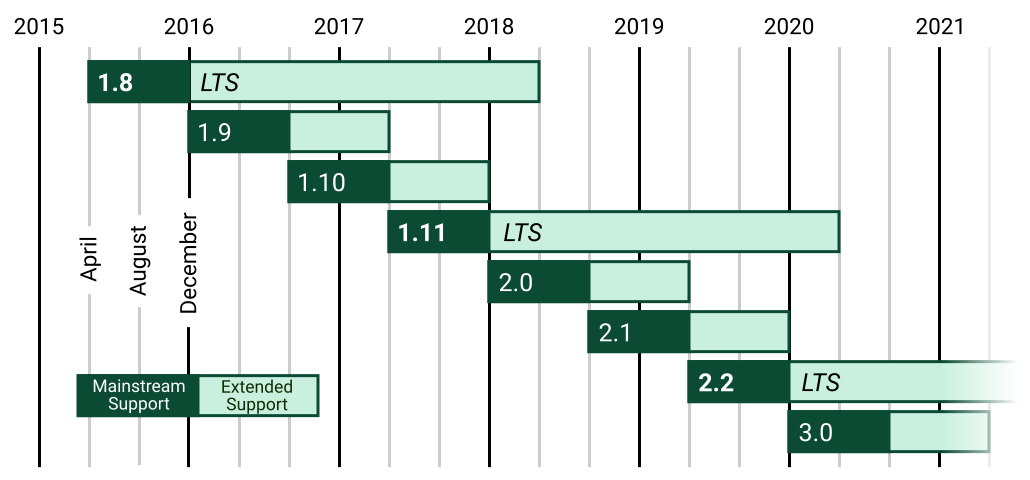
\includegraphics[width=2.5truein]{images/django-support-lts.png}


\end{figure}

La version utilisée sera une bonne indication à prendre en considération pour nos dépendances, puisqu’en visant une version particulière, nous ne devrons pratiquement pas nous soucier (bon, un peu quand même, mais nous le verrons plus tard…​) des dépendances à installer, pour peu que l’on reste sous un certain seuil.


Dans cette partie, nous allons parler de \textbf{méthodes de travail}, avec comme objectif d’éviter que l’application ne tourne que sur notre machine et que chaque déploiement ne soit une plaie à gérer.
Chaque mise à jour doit être réalisable de la manière la plus simple possible:


\begin{enumerate}

\item{démarrer un script,}

\item{prévoir un rollback si cela plante}

\item{se préparer une tisane en regardant nos flux RSS (si cette technologie existe encore…​).}

\end{enumerate}


\admonition{NOTE}{La plupart des commandes qui seront présentées dans ce livre le seront depuis un shell sous GNU/Linux. Certaines d’entre elles pourraient devoir être adaptées si vous utilisez un autre système d’exploitation (macOS) ou n’importe quelle autre grosse bouse commerciale.}
\hypertarget{x-construire-des-applications-maintenables}{\chapter{Construire des applications maintenables}}
\hypertarget{x-12-facteurs}{\section{12 facteurs}}
Pour la méthode de travail et de développement, nous allons nous baser sur les \href{https://12factor.net/fr/}{The Twelve-factor App} - ou plus simplement les \textbf{12 facteurs}.


L’idée derrière cette méthode, et indépendamment des langages de développement utilisés, consiste à suivre un ensemble de douze concepts, afin de:


\begin{enumerate}

\item{\textbf{Faciliter la mise en place de phases d’automatisation}; plus concrètement, de faciliter les mises à jour applicatives, simplifier la gestion de l’hôte, diminuer la divergence entre les différents environnements d’exécution et offrir la possibilité d’intégrer le projet dans un processus d’\href{https://en.wikipedia.org/wiki/Continuous_integration}{intégration continue} ou \href{https://en.wikipedia.org/wiki/Continuous_deployment}{déploiement continu}}

\item{\textbf{Faciliter la mise à pied de nouveaux développeurs ou de personnes souhaitant rejoindre le projet}, dans la mesure où la mise à disposition d’un environnement sera grandement facilitée.}

\item{\textbf{Minimiser les divergences entre les différents environnemens sur lesquels un projet pourrait être déployé}}

\item{\textbf{Augmenter l’agilité générale du projet}, en permettant une meilleure évolutivité architecturale et une meilleure mise à l’échelle - \emph{Vous avez 5000 utilisateurs en plus? Ajoutez un serveur et on n’en parle plus ;-)}.}

\end{enumerate}


En pratique, les points ci-dessus permettront de monter facilement un nouvel environnement - qu’il soit sur la machine du petit nouveau dans l’équipe, sur un serveur Azure, Heroku, Digital Ocean ou votre nouveau Raspberry Pi Zéro caché à la cave - et vous feront gagner un temps précieux.


Pour reprendre de manière très brute les différentes idées derrière cette méthode, nous avons:


\section{Une base de code unique, suivie par un système de contrôle de versions}


Chaque déploiement de l’application se basera sur cette source, afin de minimiser les différences que l’on pourrait trouver entre deux environnements d’un même projet. On utilisera un dépôt Git - Github, Gitlab, Gitea, …​ Au choix.


\begin{figure}[h]{}
\centering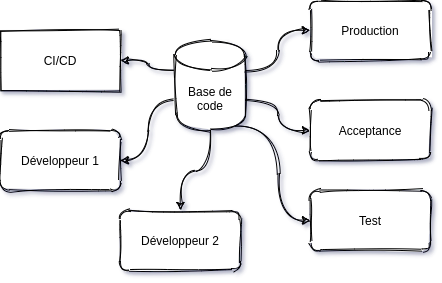
\includegraphics[width=2.5truein]{images/diagrams/12-factors-1.png}

\centering
\end{figure}

\textbf{2 - Déclarez explicitement les dépendances nécessaires au projet, et les isoler du reste du système lors de leur installation}


Chaque installation ou configuration doit toujours être faite de la même manière, et doit pouvoir être répétée quel que soit l’environnement cible.


Cela permet d’éviter que l’application n’utilise une dépendance qui soit déjà installée sur un des sytèmes de développement, et qu’elle soit difficile, voire impossible, à répercuter sur un autre environnement.
Dans notre cas, cela pourra être fait au travers de \href{https://pypi.org/project/pip/}{PIP - Package Installer for Python} ou \href{https://python-poetry.org/}{Poetry}.


Mais dans tous les cas, chaque application doit disposer d’un environnement sain, qui lui est assigné, et vu le peu de ressources que cela coûte, il ne faut pas s’en priver.


Chaque dépendance pouvant être déclarée et épinglée dans un fichier, il suffira de créer un nouvel environment vierge, puis d’utiliser ce fichier comme paramètre pour installer les prérequis au bon fonctionnement de notre application et vérifier que cet environnement est bien reproductible.


\admonition{WARNING}{Il est important de bien "épingler" les versions liées aux dépendances de l’application. Cela peut éviter des effets de bord comme une nouvelle version d’une librairie dans laquelle un bug aurait pu avoir été introduit.\footnote{Au conditionnel du futur plus-que-parfait antérieur. Mais ça arrive. Et tout le temps au mauvais moment.}}
\textbf{3 - Sauver la configuration directement au niveau de l’environnement}


Nous voulons éviter d’avoir à recompiler/redéployer l’application parce que:


\begin{enumerate}

\item{l’adresse du serveur de messagerie a été modifiée,}

\item{un protocole a changé en cours de route}

\item{la base de données a été déplacée}

\item{…​}

\end{enumerate}


En pratique, toute information susceptible de modifier un lien applicatif doit se trouver dans un fichier ou dans une variable d’environnement, et doit être facilement modifiable.
En allant un pas plus loin, cela permettra de paramétrer facilement un container, en modifiant une variable de configuration qui spécifierait la base de données sur laquelle l’application devra se connecter.


Toute clé de configuration (nom du serveur de base de données, adresse d’un service Web externe, clé d’API pour l’interrogation d’une ressource, …​) sera définie directement au niveau de l’hôte - à aucun moment, nous ne devons trouver un mot de passe en clair dans le dépôt source ou une valeur susceptible d’évoluer, écrite en dur dans le code.


\textbf{4 - Traiter les ressources externes comme des ressources attachées}


Nous parlons de bases de données, de services de mise en cache, d’API externes, …​
L’application doit être capable d’effectuer des changements au niveau de ces ressources sans que son code ne soit modifié. Nous parlons alors de \textbf{ressources attachées}, dont la présence est nécessaire au bon fonctionnement de l’application, mais pour lesquelles le \textbf{type} n’est pas obligatoirement défini.


Nous voulons par exemple "une base de données" et "une mémoire cache", et pas "une base MariaDB et une instance Memcached". De cette manière, les ressources peuvent être attachées et détachées d’un déploiement à la volée.


Si une base de données ne fonctionne pas correctement (problème matériel?), l’administrateur pourrait simplement restaurer un nouveau serveur à partir d’une précédente sauvegarde, et l’attacher à l’application sans que le code source ne soit modifié. une solution consiste à passer toutes ces informations (nom du serveur et type de base de données, clé d’authentification, …​) directement via des variables d’environnement.


\textbf{5 - Séparer proprement les phases de construction, de mise à disposition et d’exécution}


\begin{enumerate}

\item{La \textbf{construction} (\emph{build}) convertit un code source en un ensemble de fichiers exécutables, associé à une version et à une transaction dans le système de gestion de sources.}

\item{La \textbf{mise à disposition} (\emph{release}) associe cet ensemble à une configuration prête à être exécutée,}

\item{tandis que la phase d'\textbf{exécution} (\emph{run}) démarre les processus nécessaires au bon fonctionnement de l’application.}

\end{enumerate}


Parmi les solutions possibles, nous pourrions nous pourrions nous baser sur les \emph{releases} de Gitea, sur un serveur d’artefacts ou sur \href{https://fr.wikipedia.org/wiki/Capistrano_(logiciel)}{Capistrano}.


\textbf{6 - Les processus d’exécution ne doivent rien connaître ou conserver de l’état de l’application}


Toute information stockée en mémoire ou sur disque ne doit pas altérer le comportement futur de l’application, par exemple après un redémarrage non souhaité.


Pratiquement, si l’application devait rencontrer un problème, nous pourrions la redémarrer sur un autre serveur. Toute information qui aurait été stockée durant l’exécution de l’application sur le premier hôte serait donc perdue.
Si une réinitialisation devait être nécessaire, l’application ne devra pas compter sur la présence d’une information au niveau du nouveau système.


Il serait également difficile d’appliquer une mise à l’échelle de l’application si une donnée indispensable à son fonctionnement devait se trouver sur une seule machine où elle est exécutée.


\textbf{7 - Autoriser la liaison d’un port de l’application à un port du système hôte}


Les applications 12-factors sont auto-contenues et peuvent fonctionner en autonomie totale.
L’idée est qu’elles puissent être joignables grâce à un mécanisme de ponts, où l’hôte effectue la redirection vers l’un des ports ouverts par l’application, typiquement, en HTTP ou via un autre protocole.


\begin{figure}[h]{}
\centering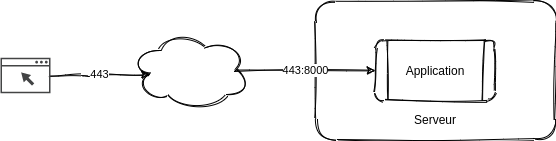
\includegraphics[width=2.5truein]{images/diagrams/12-factors-7.png}

\centering
\end{figure}

\textbf{8 - Faites confiance aux processus systèmes pour l’exécution de l’application}


Comme décrit plus haut, l’application doit utiliser des processus \emph{stateless} (sans état).
Nous pouvons créer et utiliser des processus supplémentaires pour tenir plus facilement une lourde charge, ou dédier des processus particuliers pour certaines tâches: requêtes HTTP \emph{via} des processus Web; \emph{long-running} jobs pour des processus asynchrones, …​
Si cela existe au niveau du système, ne vous fatiguez pas: utilisez le.


\textbf{9 - Améliorer la robustesse de l’application grâce à des arrêts élégants et à des démarrages rapides}


Par "arrêt élégant", nous voulons surtout éviter le \texttt{kill -9 <pid>} ou tout autre arrêt brutal d’un processus qui nécessiterait une intervention urgente du superviseur.
De cette manière, les requêtes en cours pourront se terminer au mieux, tandis que le démarrage rapide de nouveaux processus améliorera la balance d’un processus en cours d’extinction vers des processus tout frais.


L’intégration de ces mécanismes dès les premières étapes de développement limitera les perturbations et facilitera la prise en compte d’arrêts inopinés (problème matériel, redémarrage du système hôte, etc.).


\textbf{10 - Conserver les différents environnements aussi similaires que possible, et limiter les divergences entre un environnement de développement et de production}


L’exemple donné est un développeur qui utilise macOS, NGinx et SQLite, tandis que l’environnement de production tourne sur une CentOS avec Apache2 et PostgreSQL.
L’idée derrière ce concept limite les divergences entre environnements, facilite les déploiements et limite la casse et la découverte de modules non compatibles dès les premières phases de développement.


Pour vous donner un exemple tout bête, SQLite utilise un \href{https://www.sqlite.org/datatype3.html}{mécanisme de stockage dynamique}, associée à la valeur plutôt qu’au schéma, \emph{via} un système d’affinités. Un autre moteur de base de données définira un schéma statique et rigide, où la valeur sera déterminée par son contenant.
Un champ \texttt{URLField} proposé par Django a une longeur maximale par défaut de \href{https://docs.djangoproject.com/en/3.1/ref/forms/fields/#django.forms.URLField}{200 caractères}.
Si vous faites vos développements sous SQLite et que vous rencontrez une URL de plus de 200 caractères, votre développement sera passera parfaitement bien, mais plantera en production (ou en \emph{staging}, si vous faites les choses un peu mieux) parce que les données seront tronquées…​


Conserver des environements similaires limite ce genre de désagréments.


\textbf{11 - Gérer les journeaux d’évènements comme des flux}


Une application ne doit jamais se soucier de l’endroit où ses évènements seront écrits, mais simplement de les envoyer sur la sortie \texttt{stdout}.
De cette manière, que nous soyons en développement sur le poste d’un développeur avec une sortie console ou sur une machine de production avec un envoi vers une instance \href{https://www.graylog.org/}{Greylog} ou \href{https://sentry.io/welcome/}{Sentry}, le routage des journaux sera réalisé en fonction de sa nécessité et de sa criticité, et non pas parce que le développeur l’a spécifié en dur dans son code.


\textbf{12 - Isoler les tâches administratives du reste de l’application}


Evitez qu’une migration ne puisse être démarrée depuis une URL de l’application, ou qu’un envoi massif de notifications ne soit accessible pour n’importe quel utilisateur: les tâches administratives ne doivent être accessibles qu’à un administrateur.
Les applications 12facteurs favorisent les langages qui mettent un environnement REPL (pour \emph{Read}, \emph{Eval}, \emph{Print} et \emph{Loop}) à disposition (au hasard: \href{https://pythonprogramminglanguage.com/repl/}{Python} ou \href{https://kotlinlang.org/}{Kotlin}), ce qui facilite les étapes de maintenance.


\hypertarget{x-bonnes-pratiques}{\section{Bonnes pratiques}}
Pour cette section, nous nous basons sur un résumé de l’ebook \textbf{Building Maintenable Software} disponible chez \href{http://shop.oreilly.com/product/0636920049555.do}{O’Reilly}.


Ce livre répartit un ensemble de conseils parmi quatre niveaux de composants:


\begin{itemize}

\item Les méthodes et fonctions

\item Les classes

\item Les composants

\item Et des conseils plus généraux.

\end{itemize}


Ces conseils sont valables pour n’importe quel langage.


\hypertarget{x-au-niveau-des-méthodes-et-fonctions}{\subsection{Au niveau des méthodes et fonctions}}
\begin{itemize}

\item \textbf{Gardez vos méthodes/fonctions courtes}. Pas plus de 15 lignes, en comptant les commentaires. Des exceptions sont possibles, mais dans une certaine mesure uniquement (pas plus de 6.9% de plus de 60 lignes; pas plus de 22.3% de plus de 30 lignes, au plus 43.7% de plus de 15 lignes et au moins 56.3% en dessous de 15 lignes). Oui, c’est dur à tenir, mais faisable.

\item \textbf{Conserver une complexité de McCabe en dessous de 5}, c’est-à-dire avec quatre branches au maximum. A nouveau, si une méthode présente une complexité cyclomatique de 15, la séparer en 3 fonctions avec une complexité de 5 conservera globalement le nombre 15, mais rendra le code de chacune de ces méthodes plus lisible, plus maintenable.

\item \textbf{N’écrivez votre code qu’une seule fois: évitez les duplications, copie, etc.}, c’est juste mal: imaginez qu’un bug soit découvert dans une fonction; il devra alors être corrigé dans toutes les fonctions qui auront été copiées/collées. C’est aussi une forme de régression.

\item \textbf{Conservez de petites interfaces}. Quatre paramètres, pas plus. Au besoin, refactorisez certains paramètres dans une classe, qui sera plus facile à tester.

\end{itemize}


\hypertarget{x-au-niveau-des-classes}{\subsection{Au niveau des classes}}
\begin{itemize}

\item \textbf{Privilégiez un couplage faible entre vos classes}. Ceci n’est pas toujours possible, mais dans la mesure du possible, éclatez vos classes en fonction de leur domaine de compétences respectif. L’implémentation du service \texttt{UserNotificationsService} ne doit pas forcément se trouver embarqué dans une classe \texttt{UserService}. De même, pensez à passer par une interface (commune à plusieurs classes), afin d’ajouter une couche d’abstraction. La classe appellante n’aura alors que les méthodes offertes par l’interface comme points d’entrée.

\end{itemize}


\hypertarget{x-au-niveau-des-composants}{\subsection{Au niveau des composants}}
\begin{itemize}

\item \textbf{Tout comme pour les classes, il faut conserver un couplage faible au niveau des composants} également. Une manière d’arriver à ce résultat est de conserver un nombre de points d’entrée restreint, et d’éviter qu’il ne soit possible de contacter trop facilement des couches séparées de l’architecture. Pour une architecture n-tiers par exemple, la couche d’abstraction à la base de données ne peut être connue que des services; sans cela, au bout de quelques semaines, n’importe quelle couche de présentation risque de contacter directement la base de données, "\emph{juste parce qu’elle en a la possibilité}". Vous pourriez également passer par des interfaces, afin de réduire le nombre de points d’entrée connus par un composant externe (qui ne connaîtra par exemple que \texttt{IFileTransfer} avec ses méthodes \texttt{put} et \texttt{get}, et non pas les détails d’implémentation complet d’une classe \texttt{FtpFileTransfer} ou \texttt{SshFileTransfer}).

\item \textbf{Conserver un bon balancement au niveau des composants}: évitez qu’un composant \textbf{A} ne soit un énorme mastodonte, alors que le composant juste à côté ne soit capable que d’une action. De cette manière, les nouvelles fonctionnalités seront mieux réparties parmi les différents systèmes, et les responsabilités seront plus faciles à gérer. Un conseil est d’avoir un nombre de composants compris entre 6 et 12 (idéalement, 12), et que chacun de ces composants soit approximativement de même taille.

\end{itemize}


\hypertarget{x-de-manière-plus-générale}{\subsection{De manière plus générale}}
\begin{itemize}

\item \textbf{Conserver une densité de code faible}: il n’est évidemment pas possible d’implémenter n’importe quelle nouvelle fonctionnalité en moins de 20 lignes de code; l’idée ici est que la réécriture du projet ne prenne pas plus de 20 hommes/mois. Pour cela, il faut (activement) passer du temps à réduire la taille du code existant: soit en faisant du refactoring (intensif?), soit en utilisant des librairies existantes, soit en explosant un système existant en plusieurs sous-systèmes communiquant entre eux. Mais surtout, en évitant de copier/coller bêtement du code existant.

\item \textbf{Automatiser les tests}, \textbf{ajouter un environnement d’intégration continue dès le début du projet} et \textbf{vérifier par des outils les points ci-dessus}.

\end{itemize}


\hypertarget{x-solid}{\section{SOLID}}
\begin{enumerate}

\item{S : SRP (Single Responsibility}

\item{O : Open closed}

\item{L : LSP (Liskov Substitution)}

\item{I : Interface Segregation}

\item{D : Dependency Inversion}

\end{enumerate}


\hypertarget{x-single-responsibility-principle}{\subsection{Single Responsibility Principle}}
Le principe de responsabilité unique définit que chaque concept ou domaine d’activité ne s’occupe que d’une et d’une seule chose.
En prenant l’exemple d’une méthode qui communique avec une base de données, ce ne sera pas à cette méthode à gérer l’inscription d’une exception à un emplacement quelconque.
Cette action doit être prise en compte par une autre classe (ou un autre concept), qui s’occupera elle de définir l’emplacement où l’évènement sera enregistré (dans une base de données, une instance Graylog, un fichier, …​).


Cette manière d’organiser le code ajoute une couche de flemmardise (ie. Une fonction ou une méthode doit pouvoir se dire "\emph{I don’t care}" et s’occuper uniquement de ses propres oignons) sur certains concepts. Ceci permet de centraliser la configuration d’un type d’évènement à un seul endroit, ce augmente la testabilité du code.


\hypertarget{x-open-closed}{\subsection{Open Closed}}
Un des principes essentiels en programmation orientée objets concerne l’héritage de classes et la surcharge de méthodes: plutôt que de partir sur une série de comparaisons pour définir le comportement d’une instance, il est parfois préférable de définir une nouvelle sous-classe, qui surcharge une méthode bien précise.
Pour l’exemple, on pourrait ainsi définir trois classes:


\begin{itemize}

\item Une classe \texttt{Customer}, pour laquelle la méthode \texttt{GetDiscount} ne renvoit rien;

\item Une classe \texttt{SilverCustomer}, pour laquelle la méthode revoit une réduction de 10%;

\item Une classe \texttt{GoldCustomer}, pour laquelle la même méthode renvoit une réduction de 20%.

\end{itemize}


Si nous rencontrons un nouveau type de client, il suffit de créer une nouvelle sous-classe.
Cela évite d’avoir à gérer un ensemble conséquent de conditions dans la méthode initiale, en fonction d’une autre variable (ici, le type de client).


Nous passerions ainsi de:


\begin{verbatim}
class Customer():
    def __init__(self, customer_type: str):
        self.customer_type = customer_type


def get_discount(customer: Customer) -> int:
    if customer.customer_type == "Silver":
        return 10
    elif customer.customer_type == "Gold":
        return 20
    return 0


>>> jack = Customer("Silver")
>>> jack.get_discount()
10
\end{verbatim}

A ceci:


\begin{verbatim}
class Customer():
    def get_discount(self) -> int:
        return 0


class SilverCustomer(Customer):
    def get_discount(self) -> int:
        return 10


class GoldCustomer(Customer):
    def get_discount(self) -> int:
        return 20


>>> jack = SilverCustomer()
>>> jack.get_discount()
10
\end{verbatim}

En anglais, dans le texte : "Putting in simple words, the “Customer” class is now closed for any new modification but it’s open for extensions when new customer types are added to the project.". En résumé: nous fermons la classe \texttt{Customer} à toute modification, mais nous ouvrons la possibilité de créer de nouvelles extensions en ajoutant de nouveaux types [héritant de \texttt{Customer}].


De cette manière, nous simplifions également la maintenance de la méthode \texttt{get\_discount}, dans la mesure où elle dépend directement du type dans lequel elle est implémentée.


Ce point sera très utile lorsque nous aborderons les \href{https://docs.djangoproject.com/en/3.1/topics/db/models/#proxy-models}{modèles proxy}.


\hypertarget{x-liskov-substitution}{\subsection{Liskov Substitution}}
Le principe de substitution fait qu’une classe héritant d’une autre classe doit se comporter de la même manière que cette dernière.
Il n’est pas question que la sous-classe n’implémente pas certaines méthodes, alors que celles-ci sont disponibles sa classe parente.


\begin{quotation}
[…​] if S is a subtype of T, then objects of type T in a computer program may be replaced with objects of type S (i.e., objects of type S may be substituted for objects of type T), without altering any of the desirable properties of that program (correctness, task performed, etc.). (Source: \href{http://en.wikipedia.org/wiki/Liskov_substitution_principle}{Wikipédia}).
\end{quotation}

\begin{quotation}
Let q(x) be a property provable about objects x of type T. Then q(y) should be provable for objects y of type S, where S is a subtype of T. (Source: \href{http://en.wikipedia.org/wiki/Liskov_substitution_principle}{Wikipédia aussi})
\end{quotation}

Ce n’est donc pas parce qu’une classe \textbf{a besoin d’une méthode définie dans une autre classe} qu’elle doit forcément en hériter.
Cela bousillerait le principe de substitution, dans la mesure où une instance de cette classe pourra toujours être considérée comme étant du type de son parent.


Petit exemple pratique: si nous définissons une méthode \texttt{walk} et une méthode \texttt{eat} sur une classe \texttt{Duck}, et qu’une réflexion avancée (et sans doute un peu alcoolisée) nous dit que "Puisqu’un \texttt{Lion} marche aussi, faisons le hériter de notre classe `Canard`":


\begin{verbatim}
class Duck():
    def walk(self):
        print("Kwak")

    def eat(self, thing):
        if thing in ("plant", "insect", "seed", "seaweed", "fish"):
            return "Yummy!"

        raise IndigestionError("Arrrh")

class Lion(Duck):
    def walk(self):
        print("Roaaar!")
\end{verbatim}

UnNous vous laissons tester la structure ci-dessus en glissant une antilope dans la boite à goûter du lion, ce qui nous donnera quelques trucs bizarres (et un lion atteint de botulisme).


\hypertarget{x-interface-segregation}{\subsection{Interface Segregation}}
Ce principe stipule qu’un client ne peut en aucun cas dépendre d’une méthode dont il n’a pas besoin.
Plus simplement, plutôt que de dépendre d’une seule et même (grosse) interface présentant un ensemble conséquent de méthodes, il est proposé d’exploser cette interface en plusieurs (plus petites) interfaces.
Ceci permet aux différents consommateurs de n’utiliser qu’un sous-ensemble précis d’interfaces, répondant chacune à un besoin précis.


Un exemple est d’avoir une interface permettant d’accéder à des éléments.
Modifier cette interface pour permettre l’écriture impliquerait que toutes les applications ayant déjà accès à la première, obtiendraient (par défaut) un accès en écriture, ce qui n’est pas souhaité/souhaitable.


Pour contrer ceci, on aurait alors une première interface permettant la lecture, tandis qu’une deuxième (héritant de la première) permettrait l’écriture. On aurait alors le schéma suivant :


\begin{itemize}

\item A : lecture

\item B (héritant de A) : lecture (par A) et écriture.

\end{itemize}


\hypertarget{x-dependency-inversion}{\subsection{Dependency inversion}}
Dans une architecture conventionnelle, les composants de haut-niveau dépendent directement des composants de bas-niveau.
L’inversion de dépendances stipule que c’est le composant de haut-niveau qui possède la définition de l’interface dont il a besoin, et le composant de bas-niveau qui l’implémente.


Le composant de haut-niveau peut définir qu’il s’attend à avoir un \texttt{Publisher}, afin de publier du contenu vers un emplacement particulier.
Plusieurs implémentation de cette interface peuvent alors être mise en place:


\begin{itemize}

\item Une publication par SSH

\item Une publication par FTP

\item Une publication

\item …​

\end{itemize}


L’injection de dépendances est un patron de programmation qui suit le principe d’inversion de dépendances.


\hypertarget{x-sources}{\subsection{Sources}}
\begin{itemize}

\item \href{http://www.codeproject.com/Articles/703634/SOLID-architecture-principles-using-simple-Csharp}{Understanding SOLID principles on CodeProject}

\item \href{http://en.wikipedia.org/wiki/Software_craftsmanship}{Software Craftmanship}

\item \href{http://lostechies.com/derickbailey/2011/09/22/dependency-injection-is-not-the-same-as-the-dependency-inversion-principle/}{Dependency Injection is NOT the same as dependency inversion}

\item \href{http://en.wikipedia.org/wiki/Dependency_injection}{Injection de dépendances}

\end{itemize}


\hypertarget{x-complexité-de-mccabe}{\section{Complexité de McCabe}}
La \href{https://fr.wikipedia.org/wiki/Nombre_cyclomatique}{complexité cyclomatique} (ou complexité de McCabe) peut s’apparenter à mesure de difficulté de compréhension du code, en fonction du nombre d’embranchements trouvés dans une même section.
Quand le cycle d’exécution du code rencontre une condition, il peut soit rentrer dedans, soit passer directement à la suite.


Par exemple:


\begin{verbatim}
if True == False:
    pass # never happens

# continue ...
\end{verbatim}

TODO: faut vraiment reprendre un cas un peu plus lisible. Là, c’est naze.


La condition existe, mais nous ne passerons jamais dedans.
A l’inverse, le code suivant aura une complexité moisie à cause du nombre de conditions imbriquées:


\begin{verbatim}
def compare(a, b, c, d, e):
    if a == b:
        if b == c:
            if c == d:
                if d == e:
                    print('Yeah!')
                    return 1
\end{verbatim}

Potentiellement, les tests unitaires qui seront nécessaires à couvrir tous les cas de figure seront au nombre de cinq:


\begin{enumerate}

\item{le cas par défaut (a est différent de b, rien ne se passe),}

\item{le cas où \texttt{a} est égal à \texttt{b}, mais où \texttt{b} est différent de \texttt{c}}

\item{le cas où \texttt{a} est égal à \texttt{b}, \texttt{b} est égal à \texttt{c}, mais \texttt{c} est différent de \texttt{d}}

\item{le cas où \texttt{a} est égal à \texttt{b}, \texttt{b} est égal à \texttt{c}, \texttt{c} est égal à \texttt{d}, mais \texttt{d} est différent de \texttt{e}}

\item{le cas où \texttt{a} est égal à \texttt{b}, \texttt{b} est égal à \texttt{c}, \texttt{c} est égal à \texttt{d} et \texttt{d} est égal à \texttt{e}}

\end{enumerate}


La complexité cyclomatique d’un bloc est évaluée sur base du nombre d’embranchements possibles; par défaut, sa valeur est de 1.
Si nous rencontrons une condition, elle passera à 2, etc.


Pour l’exemple ci-dessous, nous allons devoir vérifier au moins chacun des cas pour nous assurer que la couverture est complète.
Nous devrions donc trouver:


\begin{enumerate}

\item{Un test où rien de se passe (\texttt{a != b})}

\item{Un test pour entrer dans la condition \texttt{a == b}}

\item{Un test pour entrer dans la condition \texttt{b == c}}

\item{Un test pour entrer dans la condition \texttt{c == d}}

\item{Un test pour entrer dans la condition \texttt{d == e}}

\end{enumerate}


Nous avons donc bien besoin de minimum cinq tests pour couvrir l’entièreté des cas présentés.


Le nombre de tests unitaires nécessaires à la couverture d’un bloc fonctionnel est au minimum égal à la complexité cyclomatique de ce bloc.
Une possibilité pour améliorer la maintenance du code est de faire baisser ce nombre, et de le conserver sous un certain seuil.
Certains recommandent de le garder sous une complexité de 10; d’autres de 5.


\admonition{NOTE}{A noter que refactoriser un bloc pour en extraire une méthode n’améliorera pas la complexité cyclomatique globale de l’application. Mais nous visons ici une amélioration \textbf{locale}.}
\hypertarget{x-boite-à-outils}{\chapter{Boite à outils}}
\hypertarget{x-python}{\section{Python}}
Le langage \href{https://www.python.org/}{Python} est un \href{https://docs.python.org/3/faq/general.html#what-is-python}{langage de programmation} interprété, interactif, orienté objet (souvent), fonctionnel (parfois), open source, multi-plateformes, flexible, facile à apprendre et difficile à maîtriser.


\begin{figure}[h]{}
\centering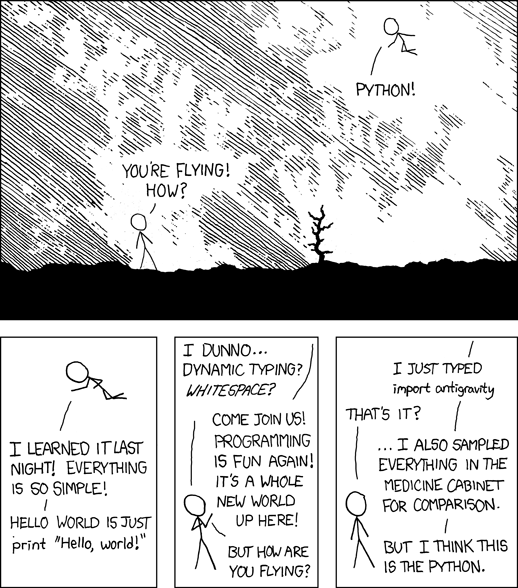
\includegraphics[width=2.5truein]{images/xkcd-353-python.png}
\caption{}

\end{figure}

A première vue, certains concepts restent difficiles à aborder: l’indentation définit l’étendue d’un bloc (classe, fonction, méthode, boucle, condition, …​), il n’y a pas de typage fort des variables et le compilateur n’est pas là pour assurer le filet de sécurité avant la mise en production (puisqu’il n’y a pas de compilateur 😛).
Et malgré ces quelques points, Python reste un langage généraliste accessible et "bon partout", et de pouvoir se reposer sur un écosystème stable et fonctionnel.


Il fonctionne avec un système d’améliorations basées sur des propositions: les PEP, ou "\textbf{Python Enhancement Proposal}".
Chacune d’entre elles doit être approuvée par le \href{http://fr.wikipedia.org/wiki/Benevolent_Dictator_for_Life}{Benevolent Dictator For Life}.


Si vous avez besoin d’un aide-mémoire ou d’une liste exhaustive des types et structures de données du langage, référez-vous au lien suivant: \href{https://gto76.github.io/python-cheatsheet/}{Python Cheat Sheet}.


\admonition{NOTE}{Le langage Python utilise un typage dynamique appelé \href{https://fr.wikipedia.org/wiki/Duck_typing}{\textbf{duck typing}}: "\emph{When I see a bird that quacks like a duck, walks like a duck, has feathers and webbed feet and associates with ducks — I’m certainly going to assume that he is a duck}"
Source: \href{http://en.wikipedia.org/wiki/Duck_test}{Wikipedia}.}
\hypertarget{x-the-zen-of-python}{\subsection{The Zen of Python}}
\begin{verbatim}
>>> import this
\end{verbatim}

\begin{verbatim}
The Zen of Python, by Tim Peters

Beautiful is better than ugly.
Explicit is better than implicit.
Simple is better than complex.
Complex is better than complicated.
Flat is better than nested.
Sparse is better than dense.
Readability counts.
Special cases aren't special enough to break the rules.
Although practicality beats purity.
Errors should never pass silently.
Unless explicitly silenced.
In the face of ambiguity, refuse the temptation to guess.
There should be one-- and preferably only one --obvious way to do it.
Although that way may not be obvious at first unless you're Dutch.
Now is better than never.
Although never is often better than *right* now.
If the implementation is hard to explain, it's a bad idea.
If the implementation is easy to explain, it may be a good idea.
Namespaces are one honking great idea -- let's do more of those!
\end{verbatim}

\hypertarget{x-pep8---style-guide-for-python-code}{\subsection{PEP8 - Style Guide for Python Code}}
La première PEP qui va nous intéresser est la \href{https://www.python.org/dev/peps/pep-0008/}{PEP 8 — Style Guide for Python Code}. Elle spécifie comment du code Python doit être organisé ou formaté, quelles sont les conventions pour l’indentation, le nommage des variables et des classes, …​
En bref, elle décrit comment écrire du code proprement, afin que d’autres développeurs puissent le reprendre facilement, ou simplement que votre base de code ne dérive lentement vers un seuil de non-maintenabilité.


Dans cet objectif, un outil existe et listera l’ensemble des conventions qui ne sont pas correctement suivies dans votre projet: pep8.
Pour l’installer, passez par pip. Lancez ensuite la commande pep8 suivie du chemin à analyser (\texttt{.}, le nom d’un répertoire, le nom d’un fichier \texttt{.py}, …​).
Si vous souhaitez uniquement avoir le nombre d’erreur de chaque type, saisissez les options \texttt{--statistics -qq}.


\begin{verbatim}
$ pep8 . --statistics -qq

7       E101 indentation contains mixed spaces and tabs
6       E122 continuation line missing indentation or outdented
8       E127 continuation line over-indented for visual indent
23      E128 continuation line under-indented for visual indent
3       E131 continuation line unaligned for hanging indent
12      E201 whitespace after '{'
13      E202 whitespace before '}'
86      E203 whitespace before ':'
\end{verbatim}

Si vous ne voulez pas être dérangé sur votre manière de coder, et que vous voulez juste avoir un retour sur une analyse de votre code, essayez \texttt{pyflakes}: cette librairie analysera vos sources à la recherche de sources d’erreurs possibles (imports inutilisés, méthodes inconnues, etc.).


\hypertarget{x-pep257---docstring-conventions}{\subsection{PEP257 - Docstring Conventions}}
Python étant un langage interprété fortement typé, il est plus que conseillé, au même titre que les tests unitaires que nous verrons plus bas, de documenter son code.
Cela impose une certaine rigueur, mais améliore énormément la qualité (et la reprise) du code par une tierce personne.
Cela implique aussi de \textbf{tout} documenter: les modules, les paquets, les classes, les fonctions, méthodes, …​
Tout doit avoir un \textbf{docstring} associé :-).


\admonition{WARNING}{Documentation: be obsessed!}
Il existe plusieurs types de conventions de documentation:


\begin{enumerate}

\item{PEP 257}

\item{Numpy}

\item{Google Style (parfois connue sous l’intitulé \texttt{Napoleon})}

\item{…​}

\end{enumerate}


Les \href{https://google.github.io/styleguide/pyguide.html#38-comments-and-docstrings}{conventions proposées par Google} nous semblent  plus faciles à lire que du RestructuredText, mais sont parfois moins bien intégrées que les docstrings officiellement supportées (typiquement, par exemple par \href{https://clize.readthedocs.io/en/stable/}{clize} qui ne reconnait que du RestructuredText).
L’exemple donné dans les styleguide est celui-ci:


\begin{verbatim}
def fetch_smalltable_rows(table_handle: smalltable.Table,
                          keys: Sequence[Union[bytes, str]],
                          require_all_keys: bool = False,
) -> Mapping[bytes, Tuple[str]]:
    """Fetches rows from a Smalltable.

    Retrieves rows pertaining to the given keys from the Table instance
    represented by table_handle.  String keys will be UTF-8 encoded.

    Args:
        table_handle: An open smalltable.Table instance.
        keys: A sequence of strings representing the key of each table
          row to fetch.  String keys will be UTF-8 encoded.
        require_all_keys: Optional; If require_all_keys is True only
          rows with values set for all keys will be returned.

    Returns:
        A dict mapping keys to the corresponding table row data
        fetched. Each row is represented as a tuple of strings. For
        example:

        {b'Serak': ('Rigel VII', 'Preparer'),
         b'Zim': ('Irk', 'Invader'),
         b'Lrrr': ('Omicron Persei 8', 'Emperor')}

        Returned keys are always bytes.  If a key from the keys argument is
        missing from the dictionary, then that row was not found in the
        table (and require_all_keys must have been False).

    Raises:
        IOError: An error occurred accessing the smalltable.
    """
\end{verbatim}

C’est-à-dire:


\begin{enumerate}

\item{Une courte ligne d’introduction, descriptive, indiquant ce que la fonction ou la méthode réalise. Attention, la documentation ne doit pas indiquer \emph{comment} la fonction/méthode est implémentée, mais ce qu’elle fait concrètement (et succintement).}

\item{Une ligne vide}

\item{Une description plus complète et plus verbeuse}

\item{Une ligne vide}

\item{La description des arguments et paramètres, des valeurs de retour (+ exemples) et les exceptions qui peuvent être levées.}

\end{enumerate}


Un exemple (encore) plus complet peut être trouvé \href{https://sphinxcontrib-napoleon.readthedocs.io/en/latest/example_google.html#example-google}{dans le dépôt sphinxcontrib-napoleon}.


Pour ceux que cela pourrait intéresser, il existe \href{https://marketplace.visualstudio.com/items?itemName=njpwerner.autodocstring}{une extension pour Codium}, comme nous le verrons juste après, qui permet de générer automatiquement le squelette de documentation d’un bloc de code:


\begin{figure}[h]{}
\centering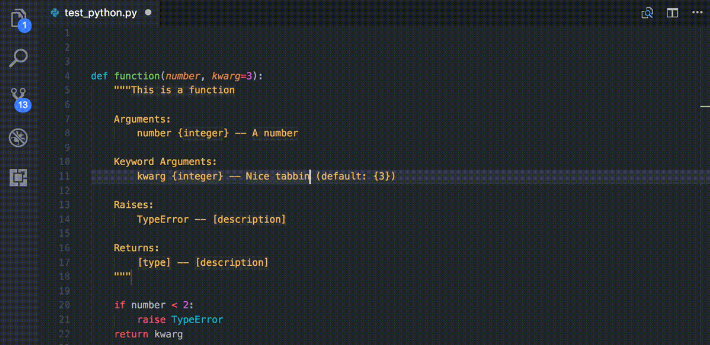
\includegraphics{images/environment/python-docstring-vscode.png}
\caption{}

\end{figure}

\admonition{NOTE}{Nous le verrons plus loin, Django permet de rendre la documentation immédiatement accessible depuis son interface d’administration.}
\hypertarget{x-linters}{\subsection{Linters}}
Il existe plusieurs niveaux de \emph{linters}:


\begin{enumerate}

\item{Le premier niveau concerne \href{https://pypi.org/project/pycodestyle/}{pycodestyle} (anciennement, \texttt{pep8} justement…​), qui analyse votre code à la recherche d’erreurs de convention.}

\item{Le deuxième niveau concerne \href{https://pypi.org/project/pyflakes/}{pyflakes}. Pyflakes est un \emph{simple} \footnote{Ce n’est pas moi qui le dit, c’est la doc du projet} programme qui recherchera des erreurs parmi vos fichiers Python.}

\item{Le troisième niveau est \href{https://pypi.org/project/flake8/}{Flake8}, qui regroupe les deux premiers niveaux, en plus d’y ajouter flexibilité, extensions et une analyse de complexité de McCabe.}

\item{Le quatrième niveau \footnote{Oui, en Python, il n’y a que quatre cercles à l’Enfer} est \href{https://pylint.org/}{PyLint}.}

\end{enumerate}


PyLint est le meilleur ami de votre \emph{moi} futur, un peu comme quand vous prenez le temps de faire la vaisselle pour ne pas avoir à la faire le lendemain: il rendra votre code soyeux et brillant, en posant des affirmations spécifiques.
A vous de les traiter en corrigeant le code ou en apposant un \emph{tag} indiquant que vous avez pris connaissance de la remarque, que vous en avez tenu compte, et que vous choisissez malgré tout de faire autrement.


Pour vous donner une idée, voici ce que cela pourrait donner avec un code pas très propre et qui ne sert à rien:


\begin{verbatim}
from datetime import datetime

"""On stocke la date du jour dans la variable ToD4y"""

ToD4y = datetime.today()

def print_today(ToD4y):
    today = ToD4y
    print(ToD4y)

def GetToday():
    return ToD4y


if __name__ == "__main__":
    t =   Get_Today()
    print(t)
\end{verbatim}

Avec Flake8, nous obtiendrons ceci:


\begin{verbatim}
test.py:7:1: E302 expected 2 blank lines, found 1
test.py:8:5: F841 local variable 'today' is assigned to but never used
test.py:11:1: E302 expected 2 blank lines, found 1
test.py:16:8: E222 multiple spaces after operator
test.py:16:11: F821 undefined name 'Get_Today'
test.py:18:1: W391 blank line at end of file
\end{verbatim}

Nous trouvons des erreurs:


\begin{itemize}

\item de \textbf{conventions}: le nombre de lignes qui séparent deux fonctions, le nombre d’espace après un opérateur, une ligne vide à la fin du fichier, …​ Ces \emph{erreurs} n’en sont pas vraiment, elles indiquent juste de potentiels problèmes de communication si le code devait être lu ou compris par une autre personne.

\item de \textbf{définition}: une variable assignée mais pas utilisée ou une lexème non trouvé. Cette dernière information indique clairement un bug potentiel. Ne pas en tenir compte nuira sans doute à la santé de votre code (et risque de vous réveiller à cinq heures du mat', quand votre application se prendra méchamment les pieds dans le tapis).

\end{itemize}


L’étape d’après consiste à invoquer pylint.
Lui, il est directement moins conciliant:


\begin{verbatim}
$ pylint test.py
************* Module test
test.py:16:6: C0326: Exactly one space required after assignment
    t =   Get_Today()
      ^ (bad-whitespace)
test.py:18:0: C0305: Trailing newlines (trailing-newlines)
test.py:1:0: C0114: Missing module docstring (missing-module-docstring)
test.py:3:0: W0105: String statement has no effect (pointless-string-statement)
test.py:5:0: C0103: Constant name "ToD4y" doesn't conform to UPPER_CASE naming style (invalid-name)
test.py:7:16: W0621: Redefining name 'ToD4y' from outer scope (line 5) (redefined-outer-name)
test.py:7:0: C0103: Argument name "ToD4y" doesn't conform to snake_case naming style (invalid-name)
test.py:7:0: C0116: Missing function or method docstring (missing-function-docstring)
test.py:8:4: W0612: Unused variable 'today' (unused-variable)
test.py:11:0: C0103: Function name "GetToday" doesn't conform to snake_case naming style (invalid-name)
test.py:11:0: C0116: Missing function or method docstring (missing-function-docstring)
test.py:16:4: C0103: Constant name "t" doesn't conform to UPPER_CASE naming style (invalid-name)
test.py:16:10: E0602: Undefined variable 'Get_Today' (undefined-variable)

--------------------------------------------------------------------
Your code has been rated at -5.45/10
\end{verbatim}

En gros, j’ai programmé comme une grosse bouse anémique (et oui: le score d’évaluation du code permet bien d’aller en négatif).
En vrac, nous trouvons des problèmes liés:


\begin{itemize}

\item au nommage (C0103) et à la mise en forme (C0305, C0326, W0105)

\item à des variables non définies (E0602)

\item de la documentation manquante (C0114, C0116)

\item de la redéfinition de variables (W0621).

\end{itemize}


Pour reprendre la \href{http://pylint.pycqa.org/en/latest/user_guide/message-control.html}{documentation}, chaque code possède sa signification (ouf!):


\begin{itemize}

\item C convention related checks

\item R refactoring related checks

\item W various warnings

\item E errors, for probable bugs in the code

\item F fatal, if an error occurred which prevented pylint from doing further* processing.

\end{itemize}


TODO: Expliquer comment faire pour tagger une explication.


TODO: Voir si la sortie de pylint est obligatoirement 0 s’il y a un warning


TODO: parler de \texttt{pylint --errors-only}


\hypertarget{x-formatage-de-code}{\subsection{Formatage de code}}
Nous avons parlé ci-dessous de style de codage pour Python (PEP8), de style de rédaction pour la documentation (PEP257), d’un \emph{linter} pour nous indiquer quels morceaux de code doivent absolument être revus, …​
Reste que ces tâches sont  (très) souvent fastidieuses: écrire un code propre et systématiquement cohérent est une tâche ardue.
Heureusement, il existe des outils pour nous aider (un peu).


A nouveau, il existe plusieurs possibilités de formatage automatique du code.
Même si elle n’est pas parfaite, \href{https://black.readthedocs.io/en/stable/}{Black} arrive à un compromis entre clarté du code, facilité d’installation et d’intégration et résultat.


Est-ce que ce formatage est idéal et accepté par tout le monde ?
\textbf{Non}. Même Pylint arrivera parfois à râler.
Mais ce formatage conviendra dans 97,83% des cas (au moins).


\begin{quotation}
By using Black, you agree to cede control over minutiae of hand-formatting. In return, Black gives you speed, determinism, and freedom from pycodestyle nagging about formatting. You will save time and mental energy for more important matters.


Black makes code review faster by producing the smallest diffs possible. Blackened code looks the same regardless of the project you’re reading. Formatting becomes transparent after a while and you can focus on the content instead.
\end{quotation}

Traduit rapidement à partir de la langue de Batman: "\emph{En utilisant Black, vous cédez le contrôle sur le formatage de votre code. En retour, Black vous fera gagner un max de temps, diminuera votre charge mentale et fera revenir l’être aimé}".
Mais la partie réellement intéressante concerne le fait que "\emph{Tout code qui sera passé par Black aura la même forme, indépendamment du project sur lequel vous serez en train de travailler. L’étape de formatage deviendra transparente, et vous pourrez vous concentrer sur le contenu}".


\hypertarget{x-complexité-cyclomatique}{\subsection{Complexité cyclomatique}}
A nouveau, un greffon pour \texttt{flake8} existe et donnera une estimation de la complexité de McCabe pour les fonctions trop complexes. Installez-le avec \texttt{pip install mccabe}, et activez-le avec le paramètre \texttt{--max-complexity}. Toute fonction dans la complexité est supérieure à cette valeur sera considérée comme trop complexe.


\hypertarget{x-typage-statique---\href{https://www.python.org/dev/peps/pep-0585/}{pep585}}{\subsection{Typage statique - \href{https://www.python.org/dev/peps/pep-0585/}{PEP585}}}
Nous vous disions ci-dessus que Python était un langage dynamique interprété.
Concrètement, cela signifie que des erreurs pouvant être détectées à la compilation avec d’autres langages, ne le sont pas avec Python.


Il existe cependant une solution à ce problème, sous la forme de \href{http://mypy-lang.org/}{Mypy}, qui peut (sous vous le souhaitez ;-)) vérifier une forme de typage statique de votre code source, grâce à une expressivité du code, basée sur des annotations (facultatives, elles aussi).


Ces vérifications se présentent de la manière suivante:


\begin{verbatim}
from typing import List


def first_int_elem(l: List[int]) -> int:
    return l[0] if l else None


if __name__ == "__main__":
    print(first_int_elem([1, 2, 3]))
    print(first_int_elem(['a', 'b', 'c']))
\end{verbatim}

Est-ce que le code ci-dessous fonctionne correctement ?
\textbf{Oui}:


\begin{verbatim}
λ python mypy-test.py
1
a
\end{verbatim}

Malgré que nos annotations déclarent une liste d’entiers, rien ne nous empêche de lui envoyer une liste de caractères, sans que cela ne lui pose de problèmes.


Est-ce que Mypy va râler ? \textbf{Oui, aussi}.
Non seulement nous retournons la valeur \texttt{None} si la liste est vide alors que nous lui annoncions un entier en sortie, mais en plus, nous l’appelons avec une liste de caractères, alors que nous nous attendions à une liste d’entiers:


\begin{verbatim}
λ mypy mypy-test.py
mypy-test.py:7: error: Incompatible return value type (got "Optional[int]", expected "int")
mypy-test.py:12: error: List item 0 has incompatible type "str"; expected "int"
mypy-test.py:12: error: List item 1 has incompatible type "str"; expected "int"
mypy-test.py:12: error: List item 2 has incompatible type "str"; expected "int"
Found 4 errors in 1 file (checked 1 source file)
\end{verbatim}

Pour corriger ceci, nous devons:


\begin{enumerate}

\item{Importer le type \texttt{Optional} et l’utiliser en sortie de notre fonction \texttt{first\_int\_elem}}

\item{Eviter de lui donner de
mauvais paramètres ;-)}

\end{enumerate}


\begin{verbatim}
from typing import List, Optional


def first_int_elem(l: List[int]) -> Optional[int]:
    return l[0] if l else None


if __name__ == "__main__":
    print(first_int_elem([1, 2, 3]))
\end{verbatim}

\begin{verbatim}
λ mypy mypy-test.py
Success: no issues found in 1 source file
\end{verbatim}

\hypertarget{x-tests-unitaires}{\subsection{Tests unitaires}}
\textbf{-> PyTest}


Comme tout bon \textbf{framework} qui se respecte, Django embarque tout un environnement facilitant le lancement de tests; chaque application est créée par défaut avec un fichier \textbf{tests.py}, qui inclut la classe \texttt{TestCase} depuis le package \texttt{django.test}:


\begin{verbatim}
from django.test import TestCase


class TestModel(TestCase):
    def test_str(self):
        raise NotImplementedError('Not implemented yet')
\end{verbatim}

Idéalement, chaque fonction ou méthode doit être testée afin de bien en valider le fonctionnement, indépendamment du reste des composants. Cela permet d’isoler chaque bloc de manière unitaire, et permet de ne pas rencontrer de régression lors de l’ajout d’une nouvelle fonctionnalité ou de la modification d’une existante.
Il existe plusieurs types de tests (intégration, comportement, …​); on ne parlera ici que des tests unitaires.


Avoir des tests, c’est bien.
S’assurer que tout est testé, c’est mieux.
C’est là qu’il est utile d’avoir le pourcentage de code couvert par les différents tests, pour savoir ce qui peut être amélioré.


Comme indiqué ci-dessus, Django propose son propre cadre de tests, au travers du package \texttt{django.tests}.
Une bonne pratique (parfois discutée) consiste cependant à switcher vers \texttt{pytest}, qui présente quelques avantages:


\begin{itemize}

\item Une syntaxe plus concise (au prix de \href{https://docs.pytest.org/en/reorganize-docs/new-docs/user/naming_conventions.html}{quelques conventions}, même si elles restent configurables): un test est une fonction, et ne doit pas obligatoirement faire partie d’une classe héritant de \texttt{TestCase} - la seule nécessité étant que cette fonction fasse partie d’un module commençant ou finissant par "test" (\texttt{test\_example.py} ou \texttt{example\_test.py}).

\item Une compatibilité avec du code Python "classique" - vous ne devrez donc retenir qu’un seul ensemble de commandes ;-)

\item Des \emph{fixtures} faciles à réutiliser entre vos différents composants

\item Une compatibilité avec le reste de l’écosystème, dont la couverture de code présentée ci-dessous.

\end{itemize}


Ainsi, après installation, il nous suffit de créer notre module \texttt{test\_models.py}, dans lequel nous allons simplement tester l’addition d’un nombre et d’une chaîne de caractères (oui, c’est complètement biesse; on est sur la partie théorique ici):


\begin{verbatim}
def test_add():
    assert 1 + 1 == "argh"
\end{verbatim}

Forcément, cela va planter.
Pour nous en assurer (dès fois que quelqu’un en doute), il nous suffit de démarrer la commande \texttt{pytest}:


\begin{verbatim}
λ pytest
============================= test session starts ====================================
platform ...
rootdir: ...
plugins: django-4.1.0
collected 1 item

gwift\test_models.py F                                                          [100%]

================================== FAILURES ==========================================
_______________________________ test_basic_add _______________________________________

    def test_basic_add():
>       assert 1 + 1 == "argh"
E       AssertionError: assert (1 + 1) == 'argh'

gwift\test_models.py:2: AssertionError

=========================== short test summary info ==================================
FAILED gwift/test_models.py::test_basic_add - AssertionError: assert (1 + 1) == 'argh'
============================== 1 failed in 0.10s =====================================
\end{verbatim}

\hypertarget{x-couverture-de-code}{\subsection{Couverture de code}}
La couverture de code est une analyse qui donne un pourcentage lié à la quantité de code couvert par les tests.
Attention qu’il ne s’agit pas de vérifier que le code est \textbf{bien} testé, mais juste de vérifier \textbf{quelle partie} du code est testée.
Le paquet \texttt{coverage} se charge d’évaluer le pourcentage de code couvert par les tests.


Avec \texttt{pytest}, il convient d’utiliser le paquet \href{https://pypi.org/project/pytest-cov/}{\texttt{pytest-cov}}, suivi de la commande \texttt{pytest --cov=gwift tests/}.


Si vous préférez rester avec le cadre de tests de Django, vous pouvez passer par le paquet \href{https://pypi.org/project/django-coverage-plugin/}{django-coverage-plugin} Ajoutez-le dans le fichier \texttt{requirements/base.txt}, et lancez une couverture de code grâce à la commande \texttt{coverage}.
La configuration peut se faire dans un fichier \texttt{.coveragerc} que vous placerez à la racine de votre projet, et qui sera lu lors de l’exécution.


\begin{verbatim}
# requirements/base.text
[...]
django_coverage_plugin
\end{verbatim}

\begin{verbatim}
# .coveragerc to control coverage.py
[run]
branch = True
omit = ../*migrations*
plugins =
    django_coverage_plugin

[report]
ignore_errors = True

[html]
directory = coverage_html_report
\end{verbatim}

\begin{verbatim}
$ coverage run --source "." manage.py test
$ coverage report

    Name                      Stmts   Miss  Cover
    ---------------------------------------------
    gwift\gwift\__init__.py       0      0   100%
    gwift\gwift\settings.py      17      0   100%
    gwift\gwift\urls.py           5      5     0%
    gwift\gwift\wsgi.py           4      4     0%
    gwift\manage.py               6      0   100%
    gwift\wish\__init__.py        0      0   100%
    gwift\wish\admin.py           1      0   100%
    gwift\wish\models.py         49     16    67%
    gwift\wish\tests.py           1      1     0%
    gwift\wish\views.py           6      6     0%
    ---------------------------------------------
    TOTAL                        89     32    64%
    ----

$ coverage html
\end{verbatim}

<--- / partie obsolète --->


Ceci vous affichera non seulement la couverture de code estimée, et générera également vos fichiers sources avec les branches non couvertes.


\hypertarget{x-matrice-de-compatibilité}{\subsection{Matrice de compatibilité}}
L’intérêt de la matrice de compatibilité consiste à spécifier un ensemble de plusieurs versions d’un même interpréteur (ici, Python), afin de s’assurer que votre application continue à fonctionner. Nous sommes donc un cran plus haut que la spécification des versions des librairies, puisque nous nous situons directement au niveau de l’interpréteur.


L’outil le plus connu est \href{https://tox.readthedocs.io/en/latest/}{Tox}, qui consiste en un outil basé sur virtualenv et qui permet:


\begin{enumerate}

\item{de vérifier que votre application s’installe correctement avec différentes versions de Python et d’interpréteurs}

\item{de démarrer des tests parmi ces différents environnements}

\end{enumerate}


\begin{verbatim}
# content of: tox.ini , put in same dir as setup.py
[tox]
envlist = py36,py37,py38,py39
skipsdist = true

[testenv]
deps =
    -r requirements/dev.txt
commands =
    pytest
\end{verbatim}

Démarrez ensuite la commande \texttt{tox}, pour démarrer la commande \texttt{pytest} sur les environnements Python 3.6, 3.7, 3.8 et 3.9, après avoir installé nos dépendances présentes dans le fichier \texttt{requirements/dev.txt}.


\admonition{WARNING}{pour que la commande ci-dessus fonctionne correctement, il sera nécessaire que vous ayez les différentes versions d’interpréteurs installées.
Ci-dessus, la commande retournera une erreur pour chaque version non trouvée, avec une erreur type \texttt{ERROR:   pyXX: InterpreterNotFound: pythonX.X}.}
\hypertarget{x-configuration-globale}{\subsection{Configuration globale}}
Décrire le fichier setup.cfg


\begin{verbatim}
$ touch setup.cfg
\end{verbatim}

\hypertarget{x-dockerfile}{\subsection{Dockerfile}}
\begin{verbatim}
# Dockerfile

# Pull base image
#FROM python:3.8
FROM python:3.8-slim-buster

# Set environment variables
ENV PYTHONDONTWRITEBYTECODE 1
ENV PYTHONUNBUFFERED 1
ENV DEBIAN_FRONTEND noninteractive
ENV ACCEPT_EULA=Y

# install Microsoft SQL Server requirements.
ENV ACCEPT_EULA=Y
RUN apt-get update -y && apt-get update \
  && apt-get install -y --no-install-recommends curl gcc g++ gnupg


# Add SQL Server ODBC Driver 17
RUN curl https://packages.microsoft.com/keys/microsoft.asc | apt-key add -
RUN curl https://packages.microsoft.com/config/debian/10/prod.list > /etc/apt/sources.list.d/mssql-release.list
RUN apt-get update \
  && apt-get install -y msodbcsql17 unixodbc-dev

# clean the install.
RUN apt-get -y clean

# Set work directory
WORKDIR /code

# Install dependencies
COPY ./requirements/base.txt /code/requirements/
RUN pip install --upgrade pip
RUN pip install -r ./requirements/base.txt

# Copy project
COPY . /code/
\end{verbatim}

\hypertarget{x-makefile}{\subsection{Makefile}}
Pour gagner un peu de temps, n’hésitez pas à créer un fichier \texttt{Makefile} que vous placerez à la racine du projet.
L’exemple ci-dessous permettra, grâce à la commande \texttt{make coverage}, d’arriver au même résultat que ci-dessus:


\begin{verbatim}
# Makefile for gwift
#

# User-friendly check for coverage
ifeq (pass:[$(shell which coverage >/dev/null 2>&1; echo $]$?), 1)
    $(error The 'coverage' command was not found. Make sure you have coverage installed)
endif

.PHONY: help coverage

help:
    @echo "  coverage to run coverage check of the source files."

coverage:
    coverage run --source='.' manage.py test; coverage report; coverage html;
    @echo "Testing of coverage in the sources finished."
\end{verbatim}

Pour la petite histoire, \texttt{make} peu sembler un peu désuet, mais reste extrêmement efficace.


\hypertarget{x-environnement-de-développement}{\section{Environnement de développement}}
Concrètement, nous pourrions tout à fait nous limiter à Notepad ou Notepad++.
Mais à moins d’aimer se fouetter avec un câble USB, nous apprécions la complétion du code, la coloration syntaxique, l’intégration des tests unitaires et d’un debugger, ainsi que deux-trois sucreries qui feront plaisir à n’importe quel développeur.


Si vous manquez d’idées ou si vous ne savez pas par où commencer:


\begin{itemize}

\item \href{https://vscodium.com/}{VSCodium}, avec les plugins \href{https://marketplace.visualstudio.com/items?itemName=ms-python.python}{Python}et \href{https://marketplace.visualstudio.com/items?itemName=eamodio.gitlens}{GitLens}

\item \href{https://www.jetbrains.com/pycharm/}{PyCharm}

\item \href{https://www.vim.org/}{Vim} avec les plugins \href{https://github.com/davidhalter/jedi-vim}{Jedi-Vim} et \href{https://github.com/preservim/nerdtree}{nerdtree}

\end{itemize}


Si vous hésitez, et même si Codium n’est pas le plus léger (la faute à \href{https://www.electronjs.org/}{Electron}…​), il fera correctement son travail (à savoir: faciliter le vôtre), en intégrant suffisament de fonctionnalités qui gâteront les papilles émoustillées du développeur impatient.


\begin{figure}[h]{}
\centering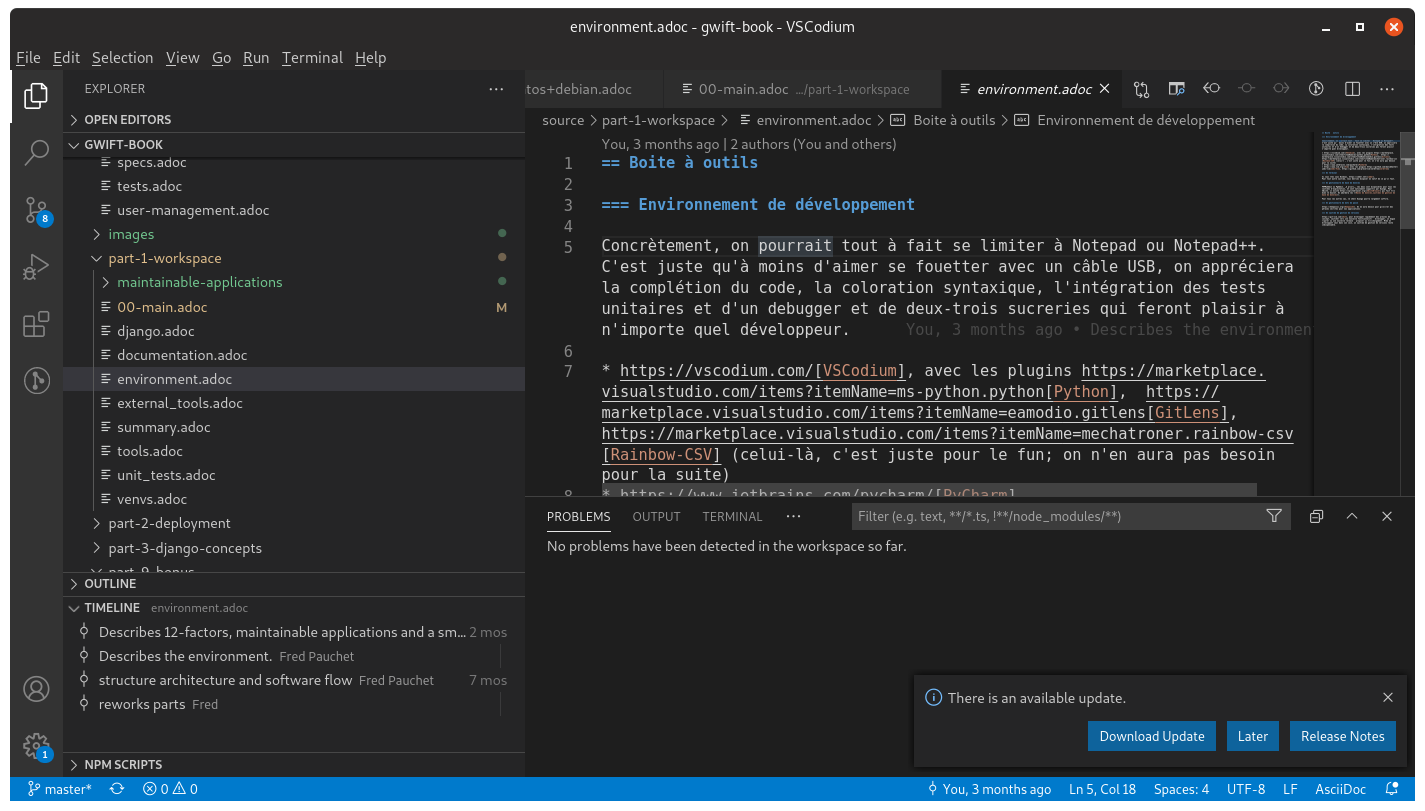
\includegraphics[width=2.5truein]{images/environment/codium.png}
\caption{}

\end{figure}

\hypertarget{x-un-terminal}{\section{Un terminal}}
\emph{A priori}, les IDE \footnote{Integrated Development Environment} proposés ci-dessus fournissent par défaut ou \emph{via} des greffons un terminal intégré.
Ceci dit, disposer d’un terminal séparé facilite parfois certaines tâches.


A nouveau, si vous manquez d’idées:


\begin{enumerate}

\item{Si vous êtes sous Windows, téléchargez une copie de \href{https://cmder.net/}{Cmder}. Il n’est pas le plus rapide, mais propose une intégration des outils Unix communs (\texttt{ls}, \texttt{pwd}, \texttt{grep}, \texttt{ssh}, \texttt{git}, …​) sans trop se fouler.}

\item{Pour tout autre système, vous devriez disposer en natif de ce qu’il faut.}

\end{enumerate}


\begin{figure}[h]{}
\centering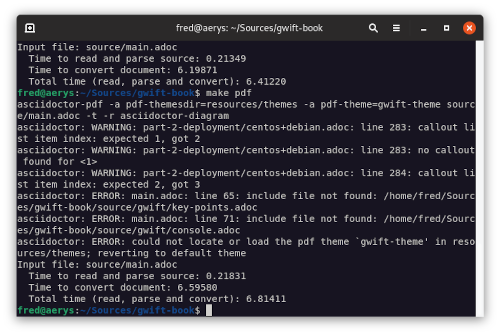
\includegraphics[width=2.5truein]{images/environment/terminal.png}
\caption{}

\end{figure}

\hypertarget{x-un-gestionnaire-de-base-de-données}{\section{Un gestionnaire de base de données}}
Django gère plusieurs moteurs de base de données.
Certains sont gérés nativement par Django (PostgreSQL, MariaDB, SQLite); \emph{a priori}, ces trois-là sont disponibles pour tous les systèmes d’exploitation. D’autres moteurs nécessitent des librairies tierces (Oracle, Microsoft SQL Server).


Il n’est pas obligatoire de disposer d’une application de gestion pour ces moteurs: pour les cas d’utilisation simples, le shell Django pourra largement suffire (nous y reviendrons).
Mais pour faciliter la gestion des bases de données elles-même, et si vous n’êtes pas à l’aise avec la ligne de commande, choisissez l’une des applications d’administration ci-dessous en fonction du moteur de base de données que vous souhaitez utiliser.


\begin{itemize}

\item Pour \textbf{PostgreSQL}, il existe \href{https://www.pgadmin.org/}{pgAdmin}

\item Pour \textbf{MariaDB} ou \textbf{MySQL}, partez sur \href{https://www.phpmyadmin.net/}{PHPMyAdmin}

\item Pour \textbf{SQLite}, il existe \href{https://sqlitebrowser.org/}{SQLiteBrowser}
PHPMyAdmin ou PgAdmin.

\end{itemize}


\hypertarget{x-un-gestionnaire-de-mots-de-passe}{\section{Un gestionnaire de mots de passe}}
Nous en auront besoin pour gé(né)rer des phrases secrètes pour nos applications.
Si vous n’en utilisez pas déjà un, partez sur \href{https://keepassxc.org/}{KeepassXC}: il est multi-plateformes, suivi et s’intègre correctement aux différents environnements, tout en restant accessible.


\begin{figure}[h]{}
\centering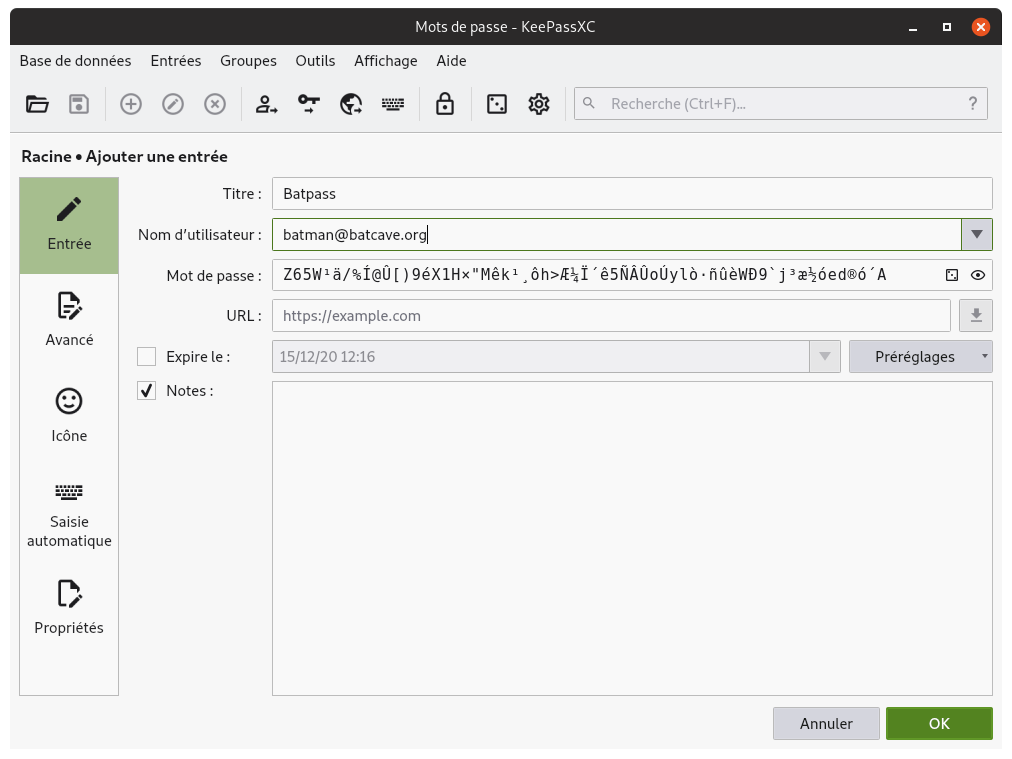
\includegraphics[width=2.5truein]{images/environment/keepass.png}


\end{figure}

\hypertarget{x-un-système-de-gestion-de-versions}{\section{Un système de gestion de versions}}
Il existe plusieurs systèmes de gestion de versions.
Le plus connu à l’heure actuelle est \href{https://git-scm.com/}{Git}, notamment pour sa (très) grande flexibilité et sa rapidité d’exécution.
Il est une aide précieuse pour développer rapidement des preuves de concept, switcher vers une nouvelle fonctionnalité, un bogue à réparer ou une nouvelle release à proposer au téléchargement.
Ses deux plus gros défauts concerneraient peut-être sa courbe d’apprentissage pour les nouveaux venus et la complexité des actions qu’il permet de réaliser.


\begin{figure}[h]{}
\centering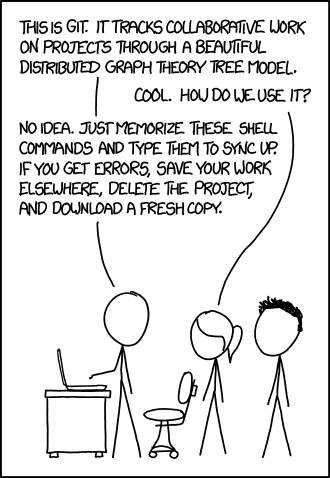
\includegraphics[width=2.5truein]{images/xkcd-1597-git.png}
\caption{}

\end{figure}

Même pour un développeur solitaire, un système de gestion de versions (quel qu’il soit) reste indispensable.


Chaque "\textbf{branche}" correspond à une tâche à réaliser: un bogue à corriger (\emph{Hotfix A}), une nouvelle fonctionnalité à ajouter ou un "\emph{truc à essayer}" \footnote{Oui, comme dans "Attends, j’essaie vite un truc, si ça marche, c’est beau."} (\emph{Feature A} et \emph{Feature B}).


Chaque "\textbf{commit}" correspond à une sauvegarde atomique d’un état ou d’un ensemble de modifications cohérentes entre elles.\footnote{Il convient donc de s’abstenir de modifier le CSS d’une application et la couche d’accès à la base de données, sous peine de se faire huer par ses relecteurs au prochain stand-up.}
De cette manière, il est beaucoup plus facile pour le développeur de se concenter sur un sujet en particulier, dans la mesure où celui-ci ne doit pas obligatoirement être clôturé pour appliquer un changement de contexte.


\begin{figure}[h]{}
\centering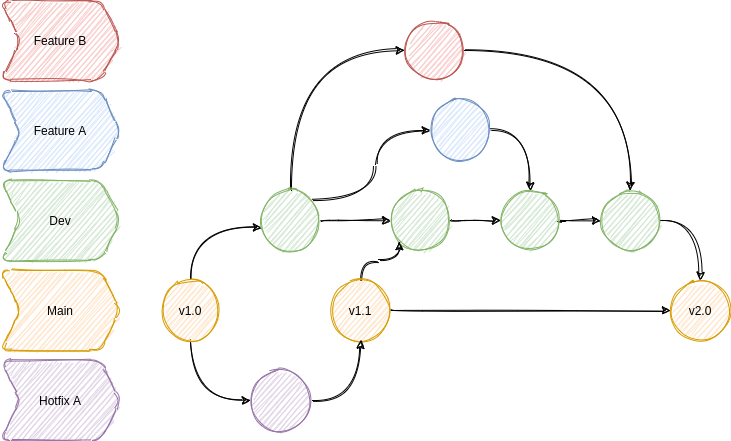
\includegraphics[width=2.5truein]{images/diagrams/git-workflow.png}
\caption{}

\end{figure}

Cas pratique: vous développez cette nouvelle fonctionnalité qui va révolutionner le monde de demain et d’après-demain, quand, tout à coup (!), vous vous rendez compte que vous avez perdu votre conformité aux normes PCI parce les données des titulaires de cartes ne sont pas isolées correctement.
Il suffit alors de:


\begin{enumerate}

\item{sauver le travail en cours (\texttt{git add \. \&\& git commit -m \[WIP\]})}

\item{revenir sur la branche principale (\texttt{git checkout main})}

\item{créer un "hotfix" (\texttt{git checkout -b hotfix/pci-compliance})}

\item{solutionner le problème (sans doute un \texttt{;} en trop ?)}

\item{sauver le correctif sur cette branche (\texttt{git add \. \&\& git commit -m \"Did it\!\"})}

\item{récupérer ce correctif sur la branche principal (\texttt{git checkout main \&\& git merge hotfix/pci-compliance})}

\item{et revenir tranquillou sur votre branche de développement pour fignoler ce générateur de noms de dinosaures rigolos que l’univers vous réclame à cor et à a cri (\texttt{git checkout features/dinolol})}

\end{enumerate}


Finalement, sachez qu’il existe plusieurs manières de gérer ces flux d’informations.
Les plus connus sont \href{https://www.gitflow.com/}{Gitflow} et \href{https://www.reddit.com/r/programming/comments/7mfxo6/a_branching_strategy_simpler_than_gitflow/}{Threeflow}.


\hypertarget{x-décrire-ses-changements}{\subsection{Décrire ses changements}}
La description d’un changement se fait \emph{via} la commande \texttt{git commit}.
Il est possible de lui passer directement le message associé à ce changement grâce à l’attribut \texttt{-m}, mais c’est une pratique relativement déconseillée: un \emph{commit} ne doit effectivement pas obligatoirement être décrit sur une seule ligne.
Une description plus complète, accompagnée des éventuels tickets ou références, sera plus complète, plus agréable à lire, et plus facile à revoir pour vos éventuels relecteurs.


De plus, la plupart des plateformes de dépôts présenteront ces informations de manière ergonomique. Par exemple:


\begin{figure}[h]{}
\centering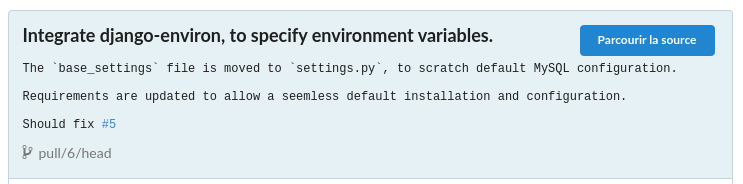
\includegraphics[width=2.5truein]{images/environment/gitea-commit-message.png}
\caption{}

\end{figure}

La première ligne est reprise comme titre (normalement, sur 50 caractères maximum); le reste est repris comme de la description.


\hypertarget{x-un-système-de-virtualisation}{\section{Un système de virtualisation}}
Par "\emph{système de virtualisation}", nous entendons n’importe quel application, système d’exploitation, système de containeurisation, …​ qui permette de créer ou recréer un environnement de développement aussi proche que celui en production.
Les solutions sont nombreuses:


\begin{itemize}

\item \href{https://www.virtualbox.org/}{VirtualBox}

\item \href{https://www.vagrantup.com/}{Vagrant}

\item \href{https://www.docker.com/}{Docker}

\item \href{https://linuxcontainers.org/lxc/}{Linux Containers (LXC)}

\item \href{https://docs.microsoft.com/fr-fr/virtualization/hyper-v-on-windows/quick-start/enable-hyper-v}{Hyper-V}

\end{itemize}


Ces quelques propositions se situent un cran plus loin que la "simple" isolation d’un environnement, puisqu’elles vous permettront de construire un environnement complet.
Elles constituent donc une étape supplémentaires dans la configuration de votre espace de travail, mais en amélioreront la qualité.


Dans la suite, nous détaillerons Vagrant et Docker, qui constituent deux solutions automatisables et multiplateformes, dont la configuration peut faire partie intégrante de vos sources.


\hypertarget{x-vagrant}{\subsection{Vagrant}}
Vagrant consiste en un outil de création et de gestion d’environnements virtualisés, en respectant toujours une même manière de travailler, indépendamment des choix techniques et de l’infrastructure que vous pourriez sélectionner.


\begin{quotation}
Vagrant is a tool for building and managing virtual machine environments in a single workflow. With an easy-to-use workflow and focus on automation, Vagrant lowers development environment setup time, increases production parity, and makes the "works on my machine" excuse a relic of the past. \footnote{\href{https://www.vagrantup.com/intro}{https://www.vagrantup.com/intro}}
\end{quotation}

La partie la plus importante de la configuration de Vagrant pour votre projet consiste à placer un fichier \texttt{Vagrantfile} - \emph{a priori} à la racine de votre projet - et qui contiendra les information suivantes:


\begin{itemize}

\item Le choix du \emph{fournisseur} (\textbf{provider}) de virtualisation (Virtualbox, Hyper-V et Docker sont natifs; il est également possible de passer par VMWare, AWS, etc.)

\item Une \emph{box}, qui consiste à lui indiquer le type et la version attendue du système virtualisé (Debian 10, Ubuntu 20.04, etc. - et \href{https://app.vagrantup.com/boxes/search}{il y a du choix}).

\item La manière dont la fourniture (\textbf{provisioning}) de l’environnement doit être réalisée: scripts Shell, fichiers, Ansible, Puppet, Chef, …​ Choisissez votre favori :-) même s’il est toujours possible de passer par une installation et une maintenance manuelle, après s’être connecté sur la machine.

\item Si un espace de stockage doit être partagé entre la machine virtuelle et l’hôte

\item Les ports qui doivent être transmis de la machine virtuelle vers l’hôte.

\end{itemize}


La syntaxe de ce fichier \texttt{Vagrantfile} est en \href{https://www.ruby-lang.org/en/}{Ruby}. Vous trouverez ci-dessous un exemple, généré (et nettoyé) après avoir exécuté la commande \texttt{vagrant init}:


\begin{verbatim}
# -*- mode: ruby -*-
# vi: set ft=ruby :
Vagrant.configure("2") do |config|

  config.vm.box = "ubuntu/bionic64"

  config.vm.network "forwarded_port", guest: 80, host: 8080, host_ip: "127.0.0.1"

  config.vm.provider "virtualbox" do |vb|
    vb.gui = true
    vb.memory = "1024"
  end

  config.vm.provision "shell", inline: <<-SHELL
    apt-get update
    apt-get install -y nginx
  SHELL
end
\end{verbatim}

Dans le fichier ci-dessus, nous créons:


\begin{itemize}

\item Une nouvelle machine virtuelle (ie. \emph{invitée}) sous Ubuntu Bionic Beaver, en x64

\item Avec une correspondance du port \texttt{80} de la machine vers le port \texttt{8080} de l’hôte, en limitant l’accès à celui-ci - accédez à \texttt{localhost:8080} et vous accéderez au port \texttt{80} de la machine virtuelle.

\item En utilisant Virtualbox comme backend - la mémoire vive allouée sera limitée à 1Go de RAM et nous ne voulons pas voir l’interface graphique au démarrage

\item Et pour finir, nous voulons appliquer un script de mise à jour \texttt{apt-get update} et installer le paquet \texttt{nginx}

\end{itemize}


\admonition{NOTE}{Par défaut, le répertoire courant (ie. le répertoire dans lequel notre fichier \texttt{Vagrantfile} se trouve) sera synchronisé dans le répertoire \texttt{/vagrant} sur la machine invitée.}
\hypertarget{x-docker}{\subsection{Docker}}
(copié/collé de cookie-cutter-django)


\begin{verbatim}
version: '3'

volumes:
  local_postgres_data: {}
  local_postgres_data_backups: {}

services:
  django: &django
    build:
      context: .
      dockerfile: ./compose/local/django/Dockerfile
    image: khana_local_django
    container_name: django
    depends_on:
      - postgres
    volumes:
      - .:/app:z
    env_file:
      - ./.envs/.local/.django
      - ./.envs/.local/.postgres
    ports:
      - "8000:8000"
    command: /start

  postgres:
    build:
      context: .
      dockerfile: ./compose/production/postgres/Dockerfile
    image: khana_production_postgres
    container_name: postgres
    volumes:
      - local_postgres_data:/var/lib/postgresql/data:Z
      - local_postgres_data_backups:/backups:z
    env_file:
      - ./.envs/.local/.postgres

  docs:
    image: khana_local_docs
    container_name: docs
    build:
      context: .
      dockerfile: ./compose/local/docs/Dockerfile
    env_file:
      - ./.envs/.local/.django
    volumes:
      - ./docs:/docs:z
      - ./config:/app/config:z
      - ./khana:/app/khana:z
    ports:
      - "7000:7000"
    command: /start-docs

  redis:
    image: redis:5.0
    container_name: redis

  celeryworker:
    <<: *django
    image: khana_local_celeryworker
    container_name: celeryworker
    depends_on:
      - redis
      - postgres

    ports: []
    command: /start-celeryworker

  celerybeat:
    <<: *django
    image: khana_local_celerybeat
    container_name: celerybeat
    depends_on:
      - redis
      - postgres

    ports: []
    command: /start-celerybeat

  flower:
    <<: *django
    image: khana_local_flower
    container_name: flower
    ports:
      - "5555:5555"
    command: /start-flower
\end{verbatim}

\begin{verbatim}
# docker-compose.yml
version: '3.8'

services:
  web:
    build: .
    command: python /code/manage.py runserver 0.0.0.0:8000
    volumes:
      - .:/code
    ports:
      - 8000:8000
    depends_on:
      - slqserver
  slqserver:
    image: mcr.microsoft.com/mssql/server:2019-latest
    environment:
      - "ACCEPT_EULA=Y"
      - "SA_PASSWORD=sqklgjqihagrtdgqk12§!"
    ports:
      - 1433:1433
    volumes:
      - ../sqlserver/data:/var/opt/mssql/data
      - ../sqlserver/log:/var/opt/mssql/log
      - ../sqlserver/secrets:/var/opt/mssql/secrets
\end{verbatim}

\begin{verbatim}
FROM python:3.8-slim-buster

ENV PYTHONUNBUFFERED 1
ENV PYTHONDONTWRITEBYTECODE 1

RUN apt-get update \
  # dependencies for building Python packages
  && apt-get install -y build-essential \
  # psycopg2 dependencies
  && apt-get install -y libpq-dev \
  # Translations dependencies
  && apt-get install -y gettext \
  # cleaning up unused files
  && apt-get purge -y --auto-remove -o APT::AutoRemove::RecommendsImportant=false \
  && rm -rf /var/lib/apt/lists/*

# Requirements are installed here to ensure they will be cached.
COPY ./requirements /requirements
RUN pip install -r /requirements/local.txt

COPY ./compose/production/django/entrypoint /entrypoint
RUN sed -i 's/\r$//g' /entrypoint
RUN chmod +x /entrypoint

COPY ./compose/local/django/start /start
RUN sed -i 's/\r$//g' /start
RUN chmod +x /start

COPY ./compose/local/django/celery/worker/start /start-celeryworker
RUN sed -i 's/\r$//g' /start-celeryworker
RUN chmod +x /start-celeryworker

COPY ./compose/local/django/celery/beat/start /start-celerybeat
RUN sed -i 's/\r$//g' /start-celerybeat
RUN chmod +x /start-celerybeat

COPY ./compose/local/django/celery/flower/start /start-flower
RUN sed -i 's/\r$//g' /start-flower
RUN chmod +x /start-flower

WORKDIR /app

ENTRYPOINT ["/entrypoint"]
\end{verbatim}

\admonition{NOTE}{Voir comment nous pouvons intégrer toutes ces commandes au niveau de la CI et au niveau du déploiement (Docker-compose ?)}
\hypertarget{x-un-projet-django}{\chapter{Un projet Django}}
\hypertarget{x-travailler-en-isolation}{\section{Travailler en isolation}}
Nous allons aborder la gestion et l’isolation des dépendances.
Cette section est aussi utile pour une personne travaillant seule, que pour transmettre les connaissances à un nouveau membre de l’équipe ou pour déployer l’application elle-même.


Il en était déjà question au deuxième point des 12 facteurs: même dans le cas de petits projets, il est déconseillé de s’en passer.
Cela évite les déploiements effectués à l’arrache à grand renfort de \texttt{sudo} et d’installation globale de dépendances, pouvant potentiellement occasioner des conflits entre les applications déployées:


\begin{enumerate}

\item{Il est tout à fait envisagable que deux applications différentes soient déployées sur un même hôte, et nécessitent chacune deux versions différentes d’une même dépendance.}

\item{Pour la reproductibilité d’un environnement spécifique, cela évite notamment les réponses type "Ca juste marche chez moi", puisque la construction d’un nouvel environnement fait partie intégrante du processus de construction et de la documentation du projet; grâce à elle, nous avons la possibilité de construire un environnement sain et d’appliquer des dépendances identiques, quelle que soit la machine hôte.}

\end{enumerate}


\begin{figure}[h]{}
\centering
\includegraphics[width=2.5truein]{images/it-works-on-my-machine.jpg}


\end{figure}

Dans la suite de ce chapitre, nous allons considérer deux projets différents:


\begin{enumerate}

\item{Gwift, une application permettant de gérer des listes de souhaits}

\item{Khana, une application de suivi d’apprentissage pour des élèves ou étudiants.}

\end{enumerate}


\hypertarget{x-environnement-virtuel}{\subsection{Environnement virtuel}}
Depuis la version 3.5 de Python, le module \texttt{venv} est \href{https://docs.python.org/3/library/venv.html}{la manière recommandée} pour créer un environnement virtuel.


\admonition{NOTE}{Il existe plusieurs autres modules permettant d’arriver au même résultat, avec quelques avantages et inconvénients pour chacun d’entre eux. Le plus prometteur d’entre eux est \href{https://python-poetry.org/}{Poetry}, qui dispose d’une interface en ligne de commande plus propre et plus moderne que ce que PIP propose.}
Pour créer un nouvel environnement, vous aurez donc besoin:


\begin{enumerate}

\item{D’une installation de Python - \href{https://www.python.org/}{https://www.python.org/}}

\item{D’un terminal - voir le point \hyperlink{../environment/-index#un-terminal}{}}

\end{enumerate}


\admonition{NOTE}{J’ai pour habitude de conserver mes projets dans un répertoire \texttt{~/Sources/} et mes environnements virtuels dans un répertoire \texttt{~/.venvs/}.
Cette séparation évite que l’environnement virtuel ne se trouve dans le même répertoire que les sources, ou ne soit accidentellement envoyé vers le système de gestion de versions.
Dans la suite de ce chapitre, je considérerai ces mêmes répertoires, mais n’hésitez pas à les modifier.}
Pur créer notre répertoire de travail et notre environnement virtuel, exécutez les commandes suivantes:


\begin{verbatim}
mkdir ~/.venvs/
python -m venv ~/.venvs/gwift-venv
\end{verbatim}

Ceci aura pour effet de créer un nouveau répertoire (\texttt{~/.venvs/gwift-env/}), dans lequel vous trouverez une installation complète de l’interpréteur Python.
Votre environnement virtuel est prêt, il n’y a plus qu’à indiquer que nous souhaitons l’utiliser, grâce à l’une des commandes suivantes:


\begin{verbatim}
# GNU/Linux, macOS
source ~/.venvs/gwift-venv/bin/activate

# MS Windows, avec Cmder
~/.venvs/gwift-venv/Scripts/activate.bat

# Pour les deux
(gwift-env) fred@aerys:~/Sources/.venvs/gwift-env$ 
\end{verbatim}


A présent que l’environnement est activé, tous les binaires de cet environnement prendront le pas sur les binaires du système.
De la même manière, une variable \texttt{PATH} propre est définie et utilisée, afin que les librairies Python y soient stockées.
C’est donc dans cet environnement virtuel que nous retrouverons le code source de Django, ainsi que des librairies externes pour Python une fois que nous les aurons installées.


\admonition{NOTE}{Pour les curieux, un environnement virtuel n’est jamais qu’un répertoire dans lequel se trouve une installation fraîche de l’interpréteur, vers laquelle pointe les liens symboliques des binaires. Si vous recherchez l’emplacement de l’interpréteur avec la commande \texttt{which python}, vous recevrez comme réponse \texttt{/home/fred/.venvs/gwift-env/bin/python}.}
Pour sortir de l’environnement virtuel, exécutez la commande \texttt{deactivate}.
Si vous pensez ne plus en avoir besoin, supprimer le dossier.
Si nécessaire, il suffira d’en créer un nouveau.


Pour gérer des versions différentes d’une même librairie, il nous suffit de jongler avec autant d’environnements que nécessaires. Une application nécessite une version de Django inférieure à la 2.0 ? On crée un environnement, on l’active et on installe ce qu’il faut.


Cette technique fonctionnera autant pour un poste de développement que sur les serveurs destinés à recevoir notre application.


\admonition{NOTE}{Par la suite, nous considérerons que l’environnement virtuel est toujours activé, même si \texttt{gwift-env} n’est pas indiqué.}
\hypertarget{x-gestion-des-dépendances,-installation-de-django-et-création-d’un-nouveau-projet}{\subsection{Gestion des dépendances, installation de Django et création d’un nouveau projet}}
Comme nous en avons déjà discuté, PIP est la solution que nous avons choisie pour la gestion de nos dépendances.
Pour installer une nouvelle librairie, vous pouvez simplement passer par la commande \texttt{pip install <my\_awesome\_library>}.
Dans le cas de Django, et après avoir activé l’environnement, nous pouvons à présent y installer Django.
Comme expliqué ci-dessus, la librairie restera indépendante du reste du système, et ne polluera aucun autre projet. nous exécuterons donc la commande suivante:


\begin{verbatim}
$ source ~/.venvs/gwift-env/bin/activate # ou ~/.venvs/gwift-env/Scrips/activate.bat pour Windows.
$ pip install django
Collecting django
    Downloading Django-3.1.4
100% |################################|
Installing collected packages: django
Successfully installed django-3.1.4
\end{verbatim}

\admonition{IMPORTANT}{Ici, la commande \texttt{pip install django} récupère la \textbf{dernière version connue disponible dans les dépôts \href{https://pypi.org/}}{https://pypi.org/}} (sauf si vous en avez définis d’autres. Mais c’est hors sujet).
Nous en avons déjà discuté: il est important de bien spécifier la version que vous souhaitez utiliser, sans quoi vous risquez de rencontrer des effets de bord.)
L’installation de Django a ajouté un nouvel exécutable: \texttt{django-admin}, que l’on peut utiliser pour créer notre nouvel espace de travail.
Par la suite, nous utiliserons \texttt{manage.py}, qui constitue un \textbf{wrapper} autour de \texttt{django-admin}.


Pour démarrer notre projet, nous lançons \texttt{django-admin startproject gwift}:


\begin{verbatim}
$ django-admin startproject gwift
\end{verbatim}

Cette action a pour effet de créer un nouveau dossier \texttt{gwift}, dans lequel nous trouvons la structure suivante:


\begin{verbatim}
$ tree gwift
gwift
├── gwift
|   |── asgi.py
│   ├── __init__.py
│   ├── settings.py
│   ├── urls.py
│   └── wsgi.py
└── manage.py
\end{verbatim}

C’est dans ce répertoire que vont vivre tous les fichiers liés au projet. Le but est de faire en sorte que toutes les opérations (maintenance, déploiement, écriture, tests, …​) puissent se faire à partir d’un seul point d’entrée.


L’utilité de ces fichiers est définie ci-dessous:


\begin{itemize}

\item \texttt{settings.py} contient tous les paramètres globaux à notre projet.

\item \texttt{urls.py} contient les variables de routes, les adresses utilisées et les fonctions vers lesquelles elles pointent.

\item \texttt{manage.py}, pour toutes les commandes de gestion.

\item \texttt{asgi.py} contient la définition de l’interface \href{https://en.wikipedia.org/wiki/Asynchronous_Server_Gateway_Interface}{ASGI}, le protocole pour la passerelle asynchrone entre votre application et le serveur Web.

\item \texttt{wsgi.py} contient la définition de l’interface \href{https://en.wikipedia.org/wiki/Web_Server_Gateway_Interface}{WSGI}, qui permettra à votre serveur Web (Nginx, Apache, …​) de faire un pont vers votre projet.

\end{itemize}


\admonition{NOTE}{Indiquer qu’il est possible d’avoir plusieurs structures de dossiers et qu’il n’y a pas de "magie" derrière toutes ces commandes.}
Tant que nous y sommes, nous pouvons ajouter un répertoire dans lequel nous stockerons les dépendances et un fichier README:


\begin{verbatim}
(gwift) $ mkdir requirements
(gwift) $ touch README.md
(gwift) $ tree gwift
gwift
├── gwift
│   ├── asgi.py
│   ├── __init__.py
│   ├── settings.py
│   ├── urls.py
│   └── wsgi.py
├── requirements 
├── README.md 
└── manage.py
\end{verbatim}


Comme nous venons d’ajouter une dépendance à notre projet, profitons-en pour créer un fichier reprenant tous les dépendances de notre projet.
Celles-ci sont normalement placées dans un fichier \texttt{requirements.txt}.
Dans un premier temps, ce fichier peut être placé directement à la racine du projet, mais on préférera rapidement le déplacer dans un sous-répertoire spécifique (\texttt{requirements}), afin de grouper les dépendances en fonction de leur environnement de destination:


\begin{itemize}

\item \texttt{base.txt}

\item \texttt{dev.txt}

\item \texttt{production.txt}

\end{itemize}


Au début de chaque fichier, il suffit d’ajouter la ligne \texttt{-r base.txt}, puis de lancer l’installation grâce à un \texttt{pip install -r <nom du fichier>}.
De cette manière, il est tout à fait acceptable de n’installer \texttt{flake8} et \texttt{django-debug-toolbar} qu’en développement par exemple.
Dans l’immédiat, nous allons ajouter \texttt{django} dans une version strictement inférieure à la version 3.2 dans le fichier \texttt{requirements/base.txt}.


\begin{verbatim}
$ echo 'django==3.2' > requirements/base.txt
$ echo '-r base.txt' > requirements/prod.txt
$ echo '-r base.txt' > requirements/dev.txt
\end{verbatim}

\admonition{IMPORTANT}{Prenez directement l’habitude de spécifier la version ou les versions compatibles: les librairies que vous utilisez comme dépendances évoluent, de la même manière que vos projets.
Pour être sûr et certain le code que vous avez écrit continue à fonctionner, spécifiez la version de chaque librairie de dépendances.
Entre deux versions d’une même librairie, des fonctions sont cassées, certaines signatures sont modifiées, des comportements sont altérés, etc. Il suffit de parcourir les pages de \emph{Changements incompatibles avec les anciennes versions dans Django} \href{https://docs.djangoproject.com/fr/3.1/releases/3.0/}{(par exemple ici pour le passage de la 3.0 à la 3.1)} pour réaliser que certaines opérations ne sont pas anodines, et que sans filet de sécurité, c’est le mur assuré.
Avec les mécanismes d’intégration continue et de tests unitaires, nous verrons plus loin comment se prémunir d’un changement inattendu.}
\hypertarget{x-django}{\section{Django}}
Comme nous l’avons vu ci-dessus, \texttt{django-admin} permet de créer un nouveau projet.
Nous faisons ici une distinction entre un \textbf{projet} et une \textbf{application}:


\begin{itemize}

\item \textbf{Un projet} représente l’ensemble des applications, paramètres, pages HTML, middlewares, dépendances, etc., qui font que votre code fait ce qu’il est sensé faire.

\item \textbf{Une application} est un contexte d’exécution, idéalement autonome, d’une partie du projet.

\end{itemize}


Pour \texttt{gwift}, nous aurons:


\begin{figure}[h]{}
\centering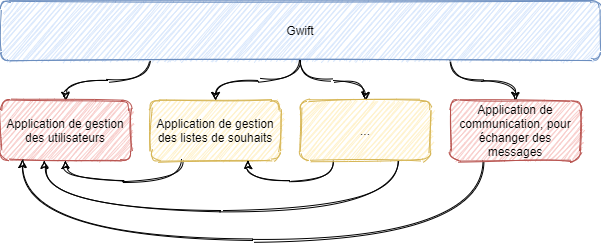
\includegraphics[width=2.5truein]{images/django/django-project-vs-apps-gwift.png}
\caption{}

\end{figure}

\begin{enumerate}

\item{une première application pour la gestion des listes de souhaits et des éléments,}

\item{une deuxième application pour la gestion des utilisateurs,}

\item{voire une troisième application qui gérera les partages entre utilisateurs et listes.}

\end{enumerate}


Nous voyons également que la gestion des listes de souhaits et éléments aura besoin de la gestion des utilisateurs - elle n’est pas autonome -, tandis que la gestion des utilisateurs n’a aucune autre dépendance qu’elle-même.


Pour \texttt{khana}, nous pourrions avoir quelque chose comme ceci:


\begin{figure}[h]{}
\centering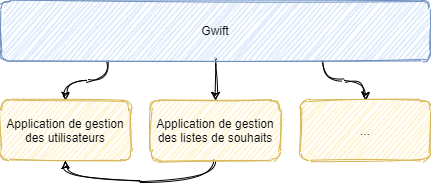
\includegraphics[width=2.5truein]{images/django/django-project-vs-apps-khana.png}
\caption{}

\end{figure}

En rouge, vous pouvez voir quelque chose que nous avons déjà vu: la gestion des utilisateurs et la possibilité qu’ils auront de communiquer entre eux.
Ceci pourrait être commun aux deux applications.
Nous pouvons clairement visualiser le principe de \textbf{contexte} pour une application: celle-ci viendra avec son modèle, ses tests, ses vues et son paramétrage et pourrait ainsi être réutilisée dans un autre projet.
C’est en ça que consistent les \href{https://www.djangopackages.com/}{paquets Django} déjà disponibles: ce sont "\emph{simplement}" de petites applications empaquetées et pouvant être réutilisées dans différents contextes (eg. \href{https://github.com/tomchristie/django-rest-framework}{Django-Rest-Framework}, \href{https://github.com/django-debug-toolbar/django-debug-toolbar}{Django-Debug-Toolbar}, …​).


\hypertarget{x-manage.py}{\subsection{manage.py}}
Le fichier \texttt{manage.py} que vous trouvez à la racine de votre projet est un \textbf{wrapper} sur les commandes \texttt{django-admin}.
A partir de maintenant, nous n’utiliserons plus que celui-là pour tout ce qui touchera à la gestion de notre projet:


\begin{itemize}

\item \texttt{manage.py check} pour vérifier (en surface…​) que votre projet ne rencontre aucune erreur évidente

\item \texttt{manage.py check --deploy}, pour vérifier (en surface aussi) que l’application est prête pour un déploiement

\item \texttt{manage.py runserver} pour lancer un serveur de développement

\item \texttt{manage.py test} pour découvrir les tests unitaires disponibles et les lancer.

\end{itemize}


La liste complète peut être affichée avec \texttt{manage.py help}.
Vous remarquerez que ces commandes sont groupées selon différentes catégories:


\begin{itemize}

\item \textbf{auth}: création d’un nouveau super-utilisateur, changer le mot de passe pour un utilisateur existant.

\item \textbf{django}: vérifier la \textbf{compliance} du projet, lancer un \textbf{shell}, \textbf{dumper} les données de la base, effectuer une migration du schéma, …​

\item \textbf{sessions}: suppressions des sessions en cours

\item \textbf{staticfiles}: gestion des fichiers statiques et lancement du serveur de développement.

\end{itemize}


Nous verrons plus tard comment ajouter de nouvelles commandes.


Si nous démarrons la commande \texttt{python manage.py runserver}, nous verrons la sortie console suivante:


\begin{verbatim}
$ python manage.py runserver
Watching for file changes with StatReloader
Performing system checks...

System check identified no issues (0 silenced).

[...]

December 15, 2020 - 20:45:07
Django version 3.1.4, using settings 'gwift.settings'
Starting development server at http://127.0.0.1:8000/
Quit the server with CTRL-BREAK.
\end{verbatim}

Si nous nous rendons sur la page \href{http://127.0.0.1:8000}{http://127.0.0.1:8000} (ou \href{http://localhost:8000}{http://localhost:8000}) comme le propose si gentiment notre (nouveau) meilleur ami, nous verrons ceci:


\begin{figure}[h]{}
\centering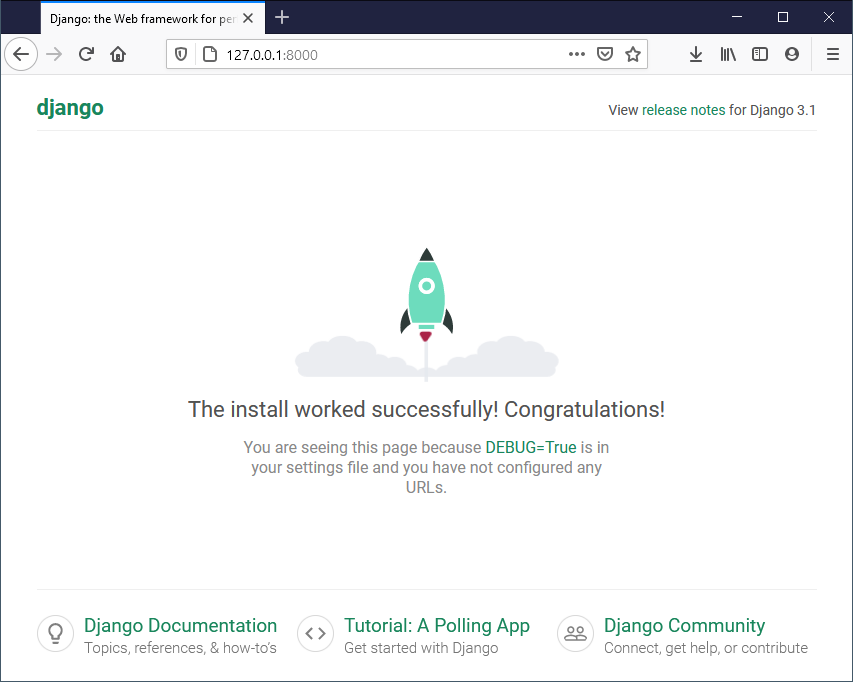
\includegraphics[width=2.5truein]{images/django/manage-runserver.png}
\caption{}

\end{figure}

\admonition{IMPORTANT}{Nous avons mis un morceau de la sortie console entre crochet \texttt{[…​]} ci-dessus, car elle concerne les migrations.
Si vous avez suivi les étapes jusqu’ici, vous avez également dû voir un message type \texttt{You have 18 unapplied migration(s). […​] Run 'python manage.py migrate' to apply them.}
Cela concerne les migrations, et c’est un point que nous verrons un peu plus tard.}
\hypertarget{x-création-d’une-nouvelle-application}{\subsection{Création d’une nouvelle application}}
Maintenant que nous avons a vu à quoi servait \texttt{manage.py}, nous pouvons créer notre nouvelle application grâce à la commande \texttt{manage.py startapp <label>}.


Notre première application servira à structurer les listes de souhaits, les éléments qui les composent et les parties que chaque utilisateur pourra offrir.
De manière générale, essayez de trouver un nom éloquent, court et qui résume bien ce que fait l’application.
Pour nous, ce sera donc \texttt{wish}.


C’est parti pour \texttt{manage.py startapp wish}!


\begin{verbatim}
$ python manage.py startapp wish
\end{verbatim}

Résultat? Django nous a créé un répertoire \texttt{wish}, dans lequel nous trouvons les fichiers et dossiers suivants:


\begin{itemize}

\item \texttt{wish/\emph{init}.py} pour que notre répertoire \texttt{wish} soit converti en package Python.

\item \texttt{wish/admin.py} servira à structurer l’administration de notre application. Chaque information peut être administrée facilement au travers d’une interface générée à la volée par le framework. Nous y reviendrons par la suite.

\item \texttt{wish/migrations/} est le dossier dans lequel seront stockées toutes les différentes migrations de notre application (= toutes les modifications que nous apporterons aux données que nous souhaiterons manipuler)

\item \texttt{wish/models.py} représentera et structurera nos données, et est intimement lié aux migrations.

\item \texttt{wish/tests.py} pour les tests unitaires.

\end{itemize}


\admonition{NOTE}{Par soucis de clarté, vous pouvez déplacer ce nouveau répertoire \texttt{wish} dans votre répertoire \texttt{gwift} existant.
C’est une forme de convention.}
La structure de vos répertoires devient celle-ci:


\begin{verbatim}
(gwift-env) fred@aerys:~/Sources/gwift$ tree .
.
├── gwift
│   ├── __init__.py
│   ├── asgi.py
│   ├── settings.py
│   ├── urls.py
│   ├── wish 
│   │   ├── __init__.py
│   │   ├── admin.py
│   │   ├── apps.py
│   │   ├── migrations
│   │   │   └── __init__.py
│   │   ├── models.py
│   │   ├── tests.py
│   │   └── views.py
│   └── wsgi.py
├── Makefile
├── manage.py
├── README.md
├── requirements
│   ├── base.txt
│   ├── dev.txt
│   └── prod.txt
├── setup.cfg
└── tox.ini

5 directories, 22 files
\end{verbatim}


\hypertarget{x-fonctionement-général}{\subsection{Fonctionement général}}
Le métier de programmeur est devenu de plus en plus complexe. Il y a 20 ans, nous pouvions nous contenter d’une simple page PHP dans laquelle nous mixions l’ensemble des actios à réaliser: requêtes en bases de données, construction de la page, …​
La recherche d’une solution a un problème n’était pas spécialement plus complexe - dans la mesure où le rendu des enregistrements en direct n’était finalement qu’une forme un chouia plus évoluée du \texttt{print()} ou des \texttt{System.out.println()} - mais c’était l’évolutivité des applications qui en prenait un coup: une grosse partie des tâches étaient dupliquées entre les différentes pages, et l’ajout d’une nouvelle fonctionnalité était relativement ardue.


Django (et d’autres cadriciels) résolvent ce problème en se basant ouvertement sur le principe de \texttt{Don’t repeat yourself} \footnote{DRY}.
Chaque morceau de code ne doit apparaitre qu’une seule fois, afin de limiter au maximum la redite (et donc, l’application d’un même correctif à différents endroits).


Le chemin parcouru par une requête est expliqué en (petits) détails ci-dessous.


\begin{figure}[h]{}
\centering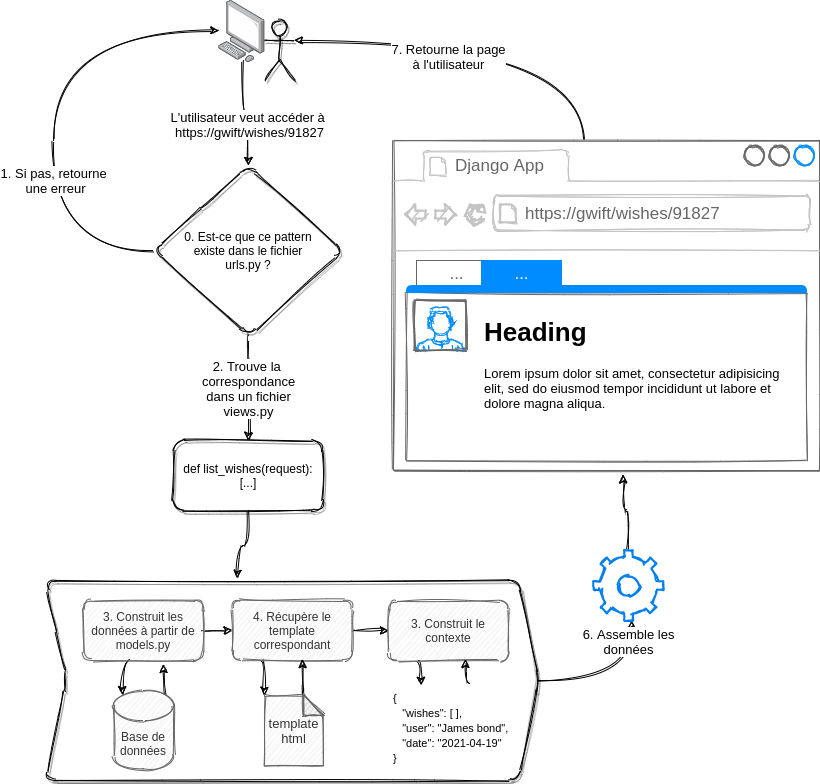
\includegraphics[width=2.5truein]{images/diagrams/django-how-it-works.png}
\caption{}

\end{figure}

\textbf{1. Un utilisateur ou un visiteur souhaite accéder à une URL hébergée et servie par notre application}.
Ici, nous prenons l’exemple de l’URL fictive \texttt{https://gwift/wishes/91827}.
Lorsque cette URL "arrive" dans notre application, son point d’entrée se trouvera au niveau des fichiers \texttt{asgi.py} ou \texttt{wsgi.py}. Nous verrons cette partie plus tard, et nous pouvons nous concentrer sur le chemin interne qu’elle va parcourir.


\textbf{Etape 0} - La première étape consiste à vérifier que cette URL répond à un schéma que nous avons défini dans le fichier \texttt{gwift/urls.py}.


\textbf{Etape 1} - Si ce n’est pas le cas, l’application n’ira pas plus loin et retournera une erreur à l’utilisateur.


\textbf{Etape 2} - Django va parcourir l’ensemble des \emph{patterns} présents dans le fichier \texttt{urls.py} et s’arrêtera sur le premier qui correspondra à la requête qu’il a reçue.
Ce cas est relativement trivial: la requête \texttt{/wishes/91827} a une correspondance au niveau de la ligne \texttt{path("wishes/<int:wish\_id>} dans l’exemple ci-dessous.
Django va alors appeler la fonction \footnote{Qui ne sera pas toujours une fonction. Django s’attend à trouver un \emph{callable}, c’est-à-dire n’importe quel élément qu’il peut appeler comme une fonction.} associée à ce \emph{pattern}, c’est-à-dire \texttt{wish\_details} du module \texttt{gwift.views}.


\begin{verbatim}
from django.contrib import admin
from django.urls import path

from gwift.views import wish_details 

urlpatterns = [
    path('admin/', admin.site.urls),
    path("wishes/<int:wish_id>", wish_details), 
]
\end{verbatim}


TODO: En fait, il faudrait quand même s’occuper du modèle ici.
TODO: et de la mise en place de l’administration, parce que nous en aurons besoin pour les étapes de déploiement.





Le module \texttt{gwift.views} qui se trouve dans le fichier \texttt{gwift/views.py} peut ressembler à ceci:


\begin{verbatim}
[...]

from datetime import datetime


def wishes_details(request: HttpRequest, wish_id: int) -> HttpResponse:
    context = {
        "user_name": "Bond,"
        "user_first_name": "James",
        "now": datetime.now()
    }

    return render(
        request,
        "wish_details.html",
        context
    )
\end{verbatim}

Pour résumer, cette fonction permet:


\begin{enumerate}

\item{De construire un \emph{contexte}, qui est représenté sous la forme d’un dictionnaire associant des clés à des valeurs. Les clés sont respectivement \texttt{user\_name}, \texttt{user\_first\_name} et \texttt{now}, tandis que leurs valeurs respectives sont \texttt{Bond}, \texttt{James} et le \texttt{moment présent} \footnote{Non, pas celui d’Eckhart Tolle}.}

\item{Nous passons ensuite ce dictionnaire à un canevas, \texttt{wish\_details.html}}

\item{L’application du contexte sur le canevas nous donne un résultat.}

\end{enumerate}


\begin{verbatim}
<!-- fichier wish_details.html -->
<!DOCTYPE html>
<html>
<head>
  <title>Page title</title>
</head>
<body>
  <h1>👤 Hi!</h1>
  <p>My name is glossterm::[ user_name ]. glossterm::[ user_first_name ] glossterm::[ user_name ].</p>
  <p>This page was generated at glossterm::[ now ]</p>
</body>
</html>
\end{verbatim}

Après application de notre contexte sur ce template, nous obtiendrons ce document, qui sera renvoyé au navigateur de l’utilisateur qui aura fait la requête initiale:


\begin{verbatim}
<!DOCTYPE html>
<html>
<head>
  <title>Page title</title>
</head>
<body>
  <h1>👤 Hi!</h1>
  <p>My name is Bond. James Bond.</p>
  <p>This page was generated at 2027-03-19 19:47:38</p>
</body>
</html>
\end{verbatim}

\begin{figure}[h]{}
\centering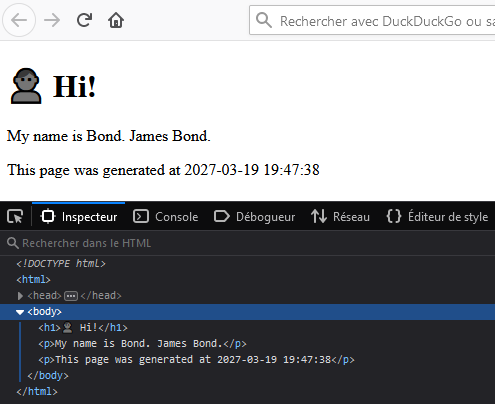
\includegraphics[width=2.5truein]{images/django/django-first-template.png}
\caption{}

\end{figure}

\hypertarget{x-12-facteurs-et-configuration-globale}{\subsection{12 facteurs et configuration globale}}
-> Faire le lien avec les settings
-> Faire le lien avec les douze facteurs
-> Construction du fichier setup.cfg


\hypertarget{x-setup.cfg}{\subsection{setup.cfg}}
(Repris de cookie-cutter-django)


\begin{verbatim}
[flake8]
max-line-length = 120
exclude = .tox,.git,*/migrations/*,*/static/CACHE/*,docs,node_modules,venv

[pycodestyle]
max-line-length = 120
exclude = .tox,.git,*/migrations/*,*/static/CACHE/*,docs,node_modules,venv

[mypy]
python_version = 3.8
check_untyped_defs = True
ignore_missing_imports = True
warn_unused_ignores = True
warn_redundant_casts = True
warn_unused_configs = True
plugins = mypy_django_plugin.main

[mypy.plugins.django-stubs]
django_settings_module = config.settings.test

[mypy-*.migrations.*]
# Django migrations should not produce any errors:
ignore_errors = True

[coverage:run]
include = khana/*
omit = *migrations*, *tests*
plugins =
    django_coverage_plugin
\end{verbatim}

\hypertarget{x-structure-finale-de-notre-environnement}{\section{Structure finale de notre environnement}}
Nous avons donc la structure finale pour notre environnement de travail:


\begin{verbatim}
(gwift-env) fred@aerys:~/Sources/gwift$ tree .
.
├── gwift
│   ├── __init__.py
│   ├── asgi.py
│   ├── settings.py
│   ├── urls.py
│   ├── wish 
│   │   ├── __init__.py
│   │   ├── admin.py
│   │   ├── apps.py
│   │   ├── migrations
│   │   │   └── __init__.py
│   │   ├── models.py
│   │   ├── tests.py
│   │   └── views.py
│   └── wsgi.py
├── Makefile
├── manage.py
├── README.md
├── requirements
│   ├── base.txt
│   ├── dev.txt
│   └── prod.txt
├── setup.cfg
└── tox.ini
\end{verbatim}

\hypertarget{x-cookie-cutter}{\section{Cookie cutter}}
Pfiou! Ca en fait des commandes et du boulot pour "juste" démarrer un nouveau projet, non? Sachant qu’en plus, nous avons dû modifier des fichiers, déplacer des dossiers, ajouter des dépendances, configurer une base de données, …​


Bonne nouvelle! Il existe des générateurs, permettant de démarrer rapidement un nouveau projet sans (trop) se prendre la tête. Le plus connu (et le plus personnalisable) est \href{https://cookiecutter.readthedocs.io/}{Cookie-Cutter}, qui se base sur des canevas \emph{type \href{https://pypi.org/project/Jinja2/}{Jinja2}}, pour créer une arborescence de dossiers et fichiers conformes à votre manière de travailler. Et si vous avez la flemme de créer votre propre canevas, vous pouvez utiliser \href{https://cookiecutter-django.readthedocs.io}{ceux qui existent déjà}.


Pour démarrer, créez un environnement virtuel (comme d’habitude):


\begin{verbatim}
λ python -m venv .venvs\cookie-cutter-khana
λ .venvs\cookie-cutter-khana\Scripts\activate.bat
(cookie-cutter-khana) λ pip install cookiecutter

  Collecting cookiecutter
  [...]
  Successfully installed Jinja2-2.11.2 MarkupSafe-1.1.1 arrow-0.17.0 binaryornot-0.4.4 certifi-2020.12.5 chardet-4.0.0 click-7.1.2 cookiecutter-1.7.2 idna-2.10 jinja2-time-0.2.0 poyo-0.5.0 python-dateutil-2.8.1 python-slugify-4.0.1 requests-2.25.1 six-1.15.0 text-unidecode-1.3 urllib3-1.26.2

(cookie-cutter-khana) λ cookiecutter https://github.com/pydanny/cookiecutter-django

  [...]

 [SUCCESS]: Project initialized, keep up the good work!
\end{verbatim}

Si vous explorez les différents fichiers, vous trouverez beaucoup de similitudes avec la configuration que nous vous proposions ci-dessus.
En fonction de votre expérience, vous serez tenté de modifier certains paramètres, pour faire correspondre ces sources avec votre utilisation ou vos habitudes.


Il est aussi possible d’utiliser l’argument \texttt{--template}, suivie d’un argument reprenant le nom de votre projet (\texttt{<my\_project>}), lors de l’initialisation d’un projet avec la commande \texttt{startproject} de \texttt{django-admin}, afin de calquer votre arborescence sur un projet existant.
La \href{https://docs.djangoproject.com/en/stable/ref/django-admin/#startproject}{documentation} à ce sujet est assez complète.

\begin{verbatim}
django-admin.py startproject --template=https://[...].zip <my_project>
\end{verbatim}

\hypertarget{x-déploiement}{\part*{Déploiement}}
Il y a une raison très simple à aborder le déploiement dès maintenant: à trop attendre et à peaufiner son développement en local, on en oublie que sa finalité sera de se retrouver exposé sur un serveur.
Il est du coup probable d’oublier une partie des désidérata, de zapper une fonctionnalité essentielle ou simplement de passer énormément de temps à adapter les sources pour qu’elles fonctionnent sur un environnement en particulier.


Aborder le déploiement dès le début permet également de rédiger dès le début les procédures d’installation, de mises à jour et de sauvegardes.
Déploier une nouvelle version sera aussi simple que de récupérer la dernière archive depuis le dépôt, la placer dans le bon répertoire, appliquer des actions spécifiques (et souvent identiques entre deux versions), puis redémarrer les services adéquats, et la procédure complète se résumera à quelques lignes d’un script bash.


Le serveur que django met à notre disposition \emph{via} la commande \texttt{runserver} est extrêmement pratique, mais il est uniquement prévu pour la phase  développement: en production, il est inutile de passer par du code Python pour charger des fichiers statiques (feuilles de style, fichiers JavaScript, images, …​).
De même, Django propose par défaut une base de données SQLite, qui fonctionne parfaitement dès lors que l’on connait ses limites et que l’on se limite à un utilisateur à la fois. En production, il est légitime que la base de donnée soit capable de supporter plusieurs utilisateurs et connexions simultanément…​
En restant avec les paramètres par défaut, il est plus que probable que vous rencontriez rapidement des erreurs de verrou parce qu’un autre processus a déjà pris la main pour écrire ses données.
En bref, vous avez quelque chose qui fonctionne, mais qui ressemble de très loin à ce dont vous aurez besoin au final.


Dans cette partie, nous aborderons les points suivants:


\begin{itemize}

\item Définir l’infrastructure nécessaire à notre application et configurer l’hôte qui hébergera l’application: dans une machine physique, virtuelle ou dans un container. Nous aborderons aussi les déploiements via Ansible et Salt.

\item Déployer notre code source

\item Configurer les outils nécessaires à la bonne exécution de ce code et de ses fonctionnalités: les différentes méthodes de supervision de l’application, comment analyser les fichiers de logs, comment intercepter correctement une erreur si elle se présente et comment remonter l’information.

\item Rendre notre application accessible depuis l’extérieur.

\end{itemize}


\hypertarget{x-infrastructure-&-composants}{\chapter{Infrastructure \& composants}}
Pour une mise ne production, le standard \emph{de facto} est le suivant:


\begin{itemize}

\item Nginx comme reverse proxy

\item HAProxy pour la distribution de charge

\item Gunicorn ou Uvicorn comme serveur d’application

\item Supervisor pour le monitoring

\item PostgreSQL ou MariaDB comme base de données.

\item Celery et RabbitMQ pour l’exécution de tâches asynchrones

\item Redis / Memcache pour la mise à en cache (et pour les sessions ? A vérifier).

\end{itemize}


Si nous schématisons l’infrastructure et le chemin parcouru par une requête, nous pourrions arriver à la synthèse suivante:


\begin{enumerate}

\item{L’utilisateur fait une requête via son navigateur (Firefox ou Chrome)}

\item{Le navigateur envoie une requête http, sa version, un verbe (GET, POST, …​), un port et éventuellement du contenu}

\item{Le firewall du serveur (Debian GNU/Linux, CentOS, …​) vérifie si la requête peut être prise en compte}

\item{La requête est transmise à l’application qui écoute sur le port (probablement 80 ou 443; et \emph{a priori} Nginx)}

\item{Elle est ensuite transmise par socket et est prise en compte par un des \emph{workers} (= un processus Python) instancié par Gunicorn. Si l’un de ces travailleurs venait à planter, il serait automatiquement réinstancié par Supervisord.}

\item{Qui la transmet ensuite à l’un de ses \emph{workers} (= un processus Python).}

\item{Après exécution, une réponse est renvoyée à l’utilisateur.}

\end{enumerate}


\begin{figure}[h]{}
\centering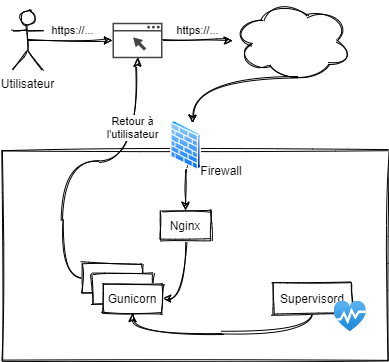
\includegraphics[width=2.5truein]{images/diagrams/architecture.png}


\end{figure}

\hypertarget{x-reverse-proxy}{\section{Reverse proxy}}
Le principe du \textbf{proxy inverse} est de pouvoir rediriger du trafic entrant vers une application hébergée sur le système.
Il serait tout à fait possible de rendre notre application directement accessible depuis l’extérieur, mais le proxy a aussi l’intérêt de pouvoir élever la sécurité du serveur (SSL) et décharger le serveur applicatif grâce à un mécanisme de cache ou en compressant certains résultats \footnote{\href{https://fr.wikipedia.org/wiki/Proxy_inverse}{https://fr.wikipedia.org/wiki/Proxy\_inverse}}


\hypertarget{x-load-balancer}{\section{Load balancer}}

\hypertarget{x-workers}{\section{Workers}}

\hypertarget{x-supervision-des-processus}{\section{Supervision des processus}}

\hypertarget{x-base-de-données}{\section{Base de données}}

\hypertarget{x-tâches-asynchrones}{\section{Tâches asynchrones}}

\hypertarget{x-mise-en-cache}{\section{Mise en cache}}

\hypertarget{x-code-source}{\chapter{Code source}}
Au niveau logiciel (la partie mise en subrillance ci-dessus), la requête arrive dans les mains du processus Python, qui doit encore


\begin{enumerate}

\item{effectuer le routage des données,}

\item{trouver la bonne fonction à exécuter,}

\item{récupérer les données depuis la base de données,}

\item{effectuer le rendu ou la conversion des données,}

\item{et renvoyer une réponse à l’utilisateur.}

\end{enumerate}


Comme nous l’avons vu dans la première partie, Django est un framework complet, intégrant tous les mécanismes nécessaires à la bonne évolution d’une application.
Il est possible de démarrer petit, et de suivre l’évolution des besoins en fonction de la charge estimée ou ressentie, d’ajouter un mécanisme de mise en cache, des logiciels de suivi, …​


\hypertarget{x-outils-de-supervision-et-de-mise-à-disposition}{\chapter{Outils de supervision et de mise à disposition}}

\hypertarget{x-méthode-de-déploiement}{\chapter{Méthode de déploiement}}
Nous allons détailler ci-dessous trois méthodes de déploiement:


\begin{itemize}

\item Sur une machine hôte, en embarquant tous les composants sur un même serveur. Ce ne sera pas idéal, puisqu’il ne sera pas possible de configurer un \emph{load balancer}, de routeur plusieurs basées de données, mais ce sera le premier cas de figure.

\item Dans des containers, avec Docker-Compose.

\item Sur une \textbf{Plateforme en tant que Service} (ou plus simplement, \textbf{PaaS}), pour faire abstraction de toute la couche de configuration du serveur.

\end{itemize}


\hypertarget{x-sur-une-machine-hôte}{\section{Sur une machine hôte}}
La première étape pour la configuration de notre hôte consiste à définir les utilisateurs et groupes de droits. Il est faut absolument éviter de faire tourner une application en tant qu’utilisateur \textbf{root}, car la moindre faille pourrait avoir des conséquences catastrophiques.


Une fois que ces utilisateurs seront configurés, nous pourrons passer à l’étape de configuration, qui consistera à:


\begin{enumerate}

\item{Déployer les sources}

\item{Démarrer un serveur implémentant une interface WSGI (\textbf{Web Server Gateway Interface}), qui sera chargé de créer autant de  travailleurs que nous le désirerons.}

\item{Démarrer un superviseur, qui se chargera de veiller à la bonne santé de nos petits travailleurs, et en créer de nouveaux s’il le juge nécessaire}

\item{Configurer un proxy inverse, qui s’occupera d’envoyer les requêtes d’un utilisateur externe à la machine hôte vers notre serveur applicatif, qui la communiquera à l’un des travailleurs.}

\end{enumerate}


La machine hôte peut être louée chez Digital Ocean, Scaleway, OVH, Vultr, …​ Il existe des dizaines d’hébergements typés VPS (\textbf{Virtual Private Server}). A vous de choisir celui qui vous convient \footnote{Personnellement, j’ai un petit faible pour Hetzner Cloud}.


\hypertarget{x-déploiement-sur-debian}{\section{Déploiement sur Debian}}
\begin{verbatim}
apt update
groupadd --system webapps 
groupadd --system gunicorn_sockets 
useradd --system --gid webapps --shell /bin/bash --home /home/gwift gwift 
mkdir -p /home/gwift 
chown gwift:webapps /home/gwift 
\end{verbatim}


\hypertarget{x-installation-des-dépendances-systèmes}{\subsection{Installation des dépendances systèmes}}
La version 3.6 de Python se trouve dans les dépôts officiels de CentOS.
Si vous souhaitez utiliser une version ultérieure, il suffit de l’installer en parallèle de la version officiellement supportée par votre distribution.


Pour CentOS, vous avez donc deux possibilités :


\begin{verbatim}
yum install python36 -y
\end{verbatim}

Ou passer par une installation alternative:


\begin{verbatim}
sudo yum -y groupinstall "Development Tools"
sudo yum -y install openssl-devel bzip2-devel libffi-devel

wget https://www.python.org/ftp/python/3.8.2/Python-3.8.2.tgz
cd Python-3.8*/
./configure --enable-optimizations
sudo make altinstall 
\end{verbatim}


\hypertarget{x-installation-de-la-base-de-données}{\subsection{Installation de la base de données}}
On l’a déjà vu, Django se base sur un pattern type \href{https://www.martinfowler.com/eaaCatalog/activeRecord.html}{ActiveRecords} pour la gestion de la persistance des données et supporte les principaux moteurs de bases de données connus:


\begin{itemize}

\item SQLite (en natif, mais Django 3.0 exige une version du moteur supérieure ou égale à la 3.8)

\item MariaDB (en natif depuis Django 3.0),

\item PostgreSQL au travers de psycopg2 (en natif aussi),

\item Microsoft SQLServer grâce aux drivers […​à compléter]

\item Oracle via \href{https://oracle.github.io/python-cx_Oracle/}{cx\_Oracle}.

\end{itemize}


\admonition{CAUTION}{Chaque pilote doit être utilisé précautionneusement ! Chaque version de Django n’est pas toujours compatible avec chacune des versions des pilotes, et chaque moteur de base de données nécessite parfois une version spécifique du pilote. Par ce fait, vous serez parfois bloqué sur une version de Django, simplement parce que votre serveur de base de données se trouvera dans une version spécifique (eg. Django 2.3 à cause d’un Oracle 12.1).}
Ci-dessous, quelques procédures d’installation pour mettre un serveur à disposition. Les deux plus simples seront MariaDB et PostgreSQL, qu’on couvrira ci-dessous. Oracle et Microsoft SQLServer se trouveront en annexes.


\hypertarget{x-postgresql}{\subsubsection{PostgreSQL}}
On commence par installer PostgreSQL.


Par exemple, dans le cas de debian, on exécute la commande suivante:


\begin{verbatim}
pass:[$$]$ aptitude install postgresql postgresql-contrib
\end{verbatim}

Ensuite, on crée un utilisateur pour la DB:


\begin{verbatim}
pass:[$$]$ su - postgres
postgres@gwift:~$ createuser --interactive -P
Enter name of role to add: gwift_user
Enter password for new role:
Enter it again:
Shall the new role be a superuser? (y/n) n
Shall the new role be allowed to create databases? (y/n) n
Shall the new role be allowed to create more new roles? (y/n) n
postgres@gwift:~$
\end{verbatim}

Finalement, on peut créer la DB:


\begin{verbatim}
postgres@gwift:~$ createdb --owner gwift_user gwift
postgres@gwift:~$ exit
logout
pass:[$$]$
\end{verbatim}

\admonition{NOTE}{penser à inclure un bidule pour les backups.}
\hypertarget{x-mariadb}{\subsubsection{MariaDB}}
Idem, installation, configuration, backup, tout ça.
A copier de grimboite, je suis sûr d’avoir des notes là-dessus.


\hypertarget{x-microsoft-sql-server}{\subsubsection{Microsoft SQL Server}}

\hypertarget{x-oracle}{\subsubsection{Oracle}}

\hypertarget{x-préparation-de-l’environnement-utilisateur}{\subsection{Préparation de l’environnement utilisateur}}
\begin{verbatim}
su - gwift
cp /etc/skel/.bashrc .
cp /etc/skel/.bash_profile .
ssh-keygen
mkdir bin
mkdir .venvs
mkdir webapps
python3.6 -m venv .venvs/gwift
source .venvs/gwift/bin/activate
cd /home/gwift/webapps
git clone ...
\end{verbatim}

La clé SSH doit ensuite être renseignée au niveau du dépôt, afin de pouvoir y accéder.


A ce stade, on devrait déjà avoir quelque chose de fonctionnel en démarrant les commandes suivantes:


\begin{verbatim}
# en tant qu'utilisateur 'gwift'

source .venvs/gwift/bin/activate
pip install -U pip
pip install -r requirements/base.txt
pip install gunicorn
cd webapps/gwift
gunicorn config.wsgi:application --bind localhost:3000 --settings=config.settings_production
\end{verbatim}

\hypertarget{x-configuration-de-l’application}{\subsection{Configuration de l’application}}
\begin{verbatim}
SECRET_KEY=<set your secret key here> 
ALLOWED_HOSTS=*
STATIC_ROOT=/var/www/gwift/static
DATABASE= 
\end{verbatim}


\hypertarget{x-création-des-répertoires-de-logs}{\subsection{Création des répertoires de logs}}
\begin{verbatim}
mkdir -p /var/www/gwift/static
\end{verbatim}

\hypertarget{x-création-du-répertoire-pour-le-socket}{\subsection{Création du répertoire pour le socket}}
Dans le fichier \texttt{/etc/tmpfiles.d/gwift.conf}:


\begin{verbatim}
D /var/run/webapps 0775 gwift gunicorn_sockets -
\end{verbatim}

Suivi de la création par systemd :


\begin{verbatim}
systemd-tmpfiles --create
\end{verbatim}

\hypertarget{x-gunicorn}{\subsection{Gunicorn}}
\begin{verbatim}
#!/bin/bash

# defines settings for gunicorn
NAME="gwift"
DJANGODIR=/home/gwift/webapps/gwift
SOCKFILE=/var/run/webapps/gunicorn_gwift.sock
USER=gwift
GROUP=gunicorn_sockets
NUM_WORKERS=5
DJANGO_SETTINGS_MODULE=config.settings_production
DJANGO_WSGI_MODULE=config.wsgi

echo "Starting $NAME as `whoami`"

source /home/gwift/.venvs/gwift/bin/activate
cd $DJANGODIR
export DJANGO_SETTINGS_MODULE=$DJANGO_SETTINGS_MODULE
export PYTHONPATH=pass:[$DJANGODIR:$]PYTHONPATH

exec gunicorn ${DJANGO_WSGI_MODULE}:application \
--name $NAME \
--workers $NUM_WORKERS \
--user $USER \
--bind=unix:$SOCKFILE \
--log-level=debug \
--log-file=-
\end{verbatim}

\hypertarget{x-supervision,-keep-alive-et-autoreload}{\subsection{Supervision, keep-alive et autoreload}}
Pour la supervision, on passe par Supervisor. Il existe d’autres superviseurs,


\begin{verbatim}
yum install supervisor -y
\end{verbatim}

On crée ensuite le fichier \texttt{/etc/supervisord.d/gwift.ini}:


\begin{verbatim}
[program:gwift]
command=/home/gwift/bin/start_gunicorn.sh
user=gwift
stdout_logfile=/var/log/gwift/gwift.log
autostart=true
autorestart=unexpected
redirect_stdout=true
redirect_stderr=true
\end{verbatim}

Et on crée les répertoires de logs, on démarre supervisord et on vérifie qu’il tourne correctement:


\begin{verbatim}
mkdir /var/log/gwift
chown gwift:nagios /var/log/gwift

systemctl enable supervisord
systemctl start supervisord.service
systemctl status supervisord.service
● supervisord.service - Process Monitoring and Control Daemon
   Loaded: loaded (/usr/lib/systemd/system/supervisord.service; enabled; vendor preset: disabled)
   Active: active (running) since Tue 2019-12-24 10:08:09 CET; 10s ago
  Process: 2304 ExecStart=/usr/bin/supervisord -c /etc/supervisord.conf (code=exited, status=0/SUCCESS)
 Main PID: 2310 (supervisord)
   CGroup: /system.slice/supervisord.service
           ├─2310 /usr/bin/python /usr/bin/supervisord -c /etc/supervisord.conf
           ├─2313 /home/gwift/.venvs/gwift/bin/python3 /home/gwift/.venvs/gwift/bin/gunicorn config.wsgi:...
           ├─2317 /home/gwift/.venvs/gwift/bin/python3 /home/gwift/.venvs/gwift/bin/gunicorn config.wsgi:...
           ├─2318 /home/gwift/.venvs/gwift/bin/python3 /home/gwift/.venvs/gwift/bin/gunicorn config.wsgi:...
           ├─2321 /home/gwift/.venvs/gwift/bin/python3 /home/gwift/.venvs/gwift/bin/gunicorn config.wsgi:...
           ├─2322 /home/gwift/.venvs/gwift/bin/python3 /home/gwift/.venvs/gwift/bin/gunicorn config.wsgi:...
           └─2323 /home/gwift/.venvs/gwift/bin/python3 /home/gwift/.venvs/gwift/bin/gunicorn config.wsgi:...
ls /var/run/webapps/
\end{verbatim}

On peut aussi vérifier que l’application est en train de tourner, à l’aide de la commande \texttt{supervisorctl}:


\begin{verbatim}
pass:[$$]$ supervisorctl status gwift
gwift                            RUNNING    pid 31983, uptime 0:01:00
\end{verbatim}

Et pour gérer le démarrage ou l’arrêt, on peut passer par les commandes suivantes:


\begin{verbatim}
pass:[$$]$ supervisorctl stop gwift
gwift: stopped
root@ks3353535:/etc/supervisor/conf.d# supervisorctl start gwift
gwift: started
root@ks3353535:/etc/supervisor/conf.d# supervisorctl restart gwift
gwift: stopped
gwift: started
\end{verbatim}

\hypertarget{x-ouverture-des-ports}{\subsection{Ouverture des ports}}
\begin{verbatim}
et 443 (HTTPS).
\end{verbatim}

\begin{verbatim}
firewall-cmd --permanent --zone=public --add-service=http 
firewall-cmd --permanent --zone=public --add-service=https 
firewall-cmd --reload
\end{verbatim}


\hypertarget{x-installation-d’nginx}{\subsection{Installation d’Nginx}}
\begin{verbatim}
yum install nginx -y
usermod -a -G gunicorn_sockets nginx
\end{verbatim}

On configure ensuite le fichier \texttt{/etc/nginx/conf.d/gwift.conf}:


\begin{verbatim}
upstream gwift_app {
        server unix:/var/run/webapps/gunicorn_gwift.sock fail_timeout=0;
}

server {
        listen 80;
        server_name <server_name>;
        root /var/www/gwift;
        error_log /var/log/nginx/gwift_error.log;
        access_log /var/log/nginx/gwift_access.log;

        client_max_body_size 4G;
        keepalive_timeout 5;

        gzip on;
        gzip_comp_level 7;
        gzip_proxied any;
        gzip_types gzip_types text/plain text/css text/xml text/javascript application/x-javascript application/xml;


        location /static/ { 
                access_log off;
                expires 30d;
                add_header Pragma public;
                add_header Cache-Control "public";
                add_header Vary "Accept-Encoding";
                try_files pass:[$uri $]uri/ =404;
        }

        location / {
                proxy_set_header X-Forwarded-For $proxy_add_x_forwarded_for; 
                proxy_set_header Host $http_host;
                proxy_redirect off;

                proxy_pass http://gwift_app;
        }
}
\end{verbatim}


\hypertarget{x-mise-à-jour}{\subsection{Mise à jour}}
Script de mise à jour.


\begin{verbatim}
su - <user>
source ~/.venvs/<app>/bin/activate
cd ~/webapps/<app>
git fetch
git checkout vX.Y.Z
pip install -U requirements/prod.txt
python manage.py migrate
python manage.py collectstatic
kill -HUP `ps -C gunicorn fch -o pid | head -n 1` 
\end{verbatim}


\hypertarget{x-configuration-des-sauvegardes}{\subsection{Configuration des sauvegardes}}
Les sauvegardes ont été configurées avec borg: \texttt{yum install borgbackup}.


C’est l’utilisateur gwift qui s’en occupe.


\begin{verbatim}
mkdir -p /home/gwift/borg-backups/
cd /home/gwift/borg-backups/
borg init gwift.borg -e=none
borg create gwift.borg::{now} ~/bin ~/webapps
\end{verbatim}

Et dans le fichier crontab :


\begin{verbatim}
0 23 * * * /home/gwift/bin/backup.sh
\end{verbatim}

\hypertarget{x-rotation-des-jounaux}{\subsection{Rotation des jounaux}}
\begin{verbatim}
/var/log/gwift/* {
        weekly
        rotate 3
        size 10M
        compress
        delaycompress
}
\end{verbatim}

Puis on démarre logrotate avec \# logrotate -d /etc/logrotate.d/gwift pour vérifier que cela fonctionne correctement.


\hypertarget{x-ansible}{\subsection{Ansible}}
TODO


\hypertarget{x-heroku}{\section{Heroku}}
\href{https://www.heroku.com}{Heroku} est une \emph{Plateform As A Service} \footnote{Aussi abrégé "PaaS" pour les conaisseurs}, où vous choisissez le \emph{service} dont vous avez besoin (une base de données, un service de cache, un service applicatif, …​), vous lui envoyer les paramètres nécessaires et le tout démarre gentiment sans que vous ne deviez superviser l’hôte.
Ce mode démarrage ressemble énormément aux 12 facteurs dont nous avons déjà parlé plus tôt - raison de plus pour que notre application soit directement prête à y être déployée, d’autant plus qu’il ne sera pas possible de modifier un fichier une fois qu’elle aura démarré: si vous souhaitez modifier un paramètre, cela reviendra à couper l’actuelle et envoyer de nouveaux paramètres et recommencer le déploiement depuis le début.


\begin{figure}[h]{}
\centering
\includegraphics[width=2.5truein]{images/deployment/heroku.png}
\caption{}

\end{figure}

Pour un projet de type "hobby" et pour l’exemple de déploiement ci-dessous, il est tout à fait possible de s’en sortir sans dépenser un kopek, afin de tester nos quelques idées ou mettre rapidement un \emph{Most Valuable Product} en place. La seule contrainte consistera à pouvoir héberger des fichiers envoyés par vos utilisateurs - ceci pourra être fait en configurant un \emph{bucket S3} chez Amazon (beurk), Scaleway ou OVH \footnote{Entre autres.}


Le fonctionnement est relativement simple: pour chaque application, Heroku crée un dépôt Git qui lui est associé. Au travers de la commande \texttt{heroku create}, vous associez en fait une nouvelle référence à votre code source:


\begin{verbatim}
$ heroku create
Creating app... done, ⬢ young-temple-86098
https://young-temple-86098.herokuapp.com/ | https://git.heroku.com/young-temple-86098.git

$ cat .git/config
[core]
        repositoryformatversion = 0
        filemode = false
        bare = false
        logallrefupdates = true
        symlinks = false
        ignorecase = true
[remote "heroku"]
        url = https://git.heroku.com/still-thicket-66406.git
        fetch = +refs/heads/*:refs/remotes/heroku/*
\end{verbatim}

Pour envoyer une nouvelle version, il suffit dès lors (après l’avoir paramétrée), de pousser la référence grâce à la commande \texttt{git push heroku master}.


Prêt à vous lancer ? Commencez par créer un compte: \href{https://signup.heroku.com/python}{https://signup.heroku.com/python}.


\hypertarget{x-configuration-du-compte-heroku}{\subsection{Configuration du compte Heroku}}
+ Récupération des valeurs d’environnement pour les réutiliser ci-dessous.


Vous aurez peut-être besoin d’un coup de pouce pour démarrer votre première application; heureusement, la documentation est super bien faite:


\begin{figure}[h]{}
\centering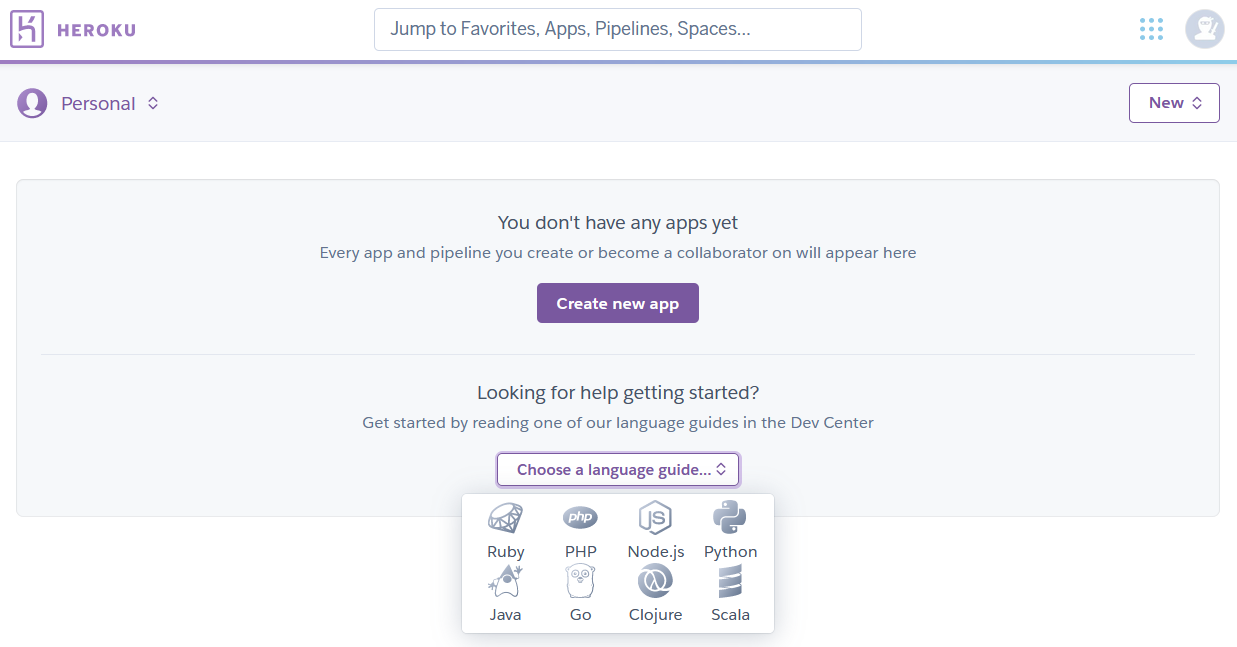
\includegraphics[width=2.5truein]{images/deployment/heroku-new-app.png}
\caption{}

\end{figure}

Installez ensuite la CLI (\emph{Command Line Interface}) en suivant \href{https://devcenter.heroku.com/articles/heroku-cli}{la documentation suivante}.


Au besoin, cette CLI existe pour:


\begin{enumerate}

\item{macOS, \emph{via} `brew `}

\item{Windows, grâce à un \href{https://cli-assets.heroku.com/heroku-x64.exe}{binaire x64} (la version 32 bits existe aussi, mais il est peu probable que vous en ayez besoin)}

\item{GNU/Linux, via un script Shell \texttt{curl \href{https://cli-assets.heroku.com/install.sh}{https://cli-assets.heroku.com/install.sh} | sh} ou sur \href{https://snapcraft.io/heroku}{SnapCraft}.}

\end{enumerate}


Une fois installée, connectez-vous:


\begin{verbatim}
$ heroku login
\end{verbatim}

Et créer votre application:


\begin{verbatim}
$ heroku create
Creating app... done, ⬢ young-temple-86098
https://young-temple-86098.herokuapp.com/ | https://git.heroku.com/young-temple-86098.git
\end{verbatim}

\begin{figure}[h]{}
\centering
\includegraphics[width=2.5truein]{images/deployment/heroku-app-created.png}
\caption{}

\end{figure}

Ajoutons lui une base de données, que nous sauvegarderons à intervalle régulier:


\begin{verbatim}
$ heroku addons:create heroku-postgresql:hobby-dev
Creating heroku-postgresql:hobby-dev on ⬢ still-thicket-66406... free
Database has been created and is available
 ! This database is empty. If upgrading, you can transfer
 ! data from another database with pg:copy
Created postgresql-clear-39693 as DATABASE_URL
Use heroku addons:docs heroku-postgresql to view documentation

$ heroku pg:backups schedule --at '14:00 Europe/Brussels' DATABASE_URL
Scheduling automatic daily backups of postgresql-clear-39693 at 14:00 Europe/Brussels... done
\end{verbatim}

TODO: voir comment récupérer le backup de la db :-p


\begin{verbatim}
# Copié/collé de https://cookiecutter-django.readthedocs.io/en/latest/deployment-on-heroku.html
heroku create --buildpack https://github.com/heroku/heroku-buildpack-python

heroku addons:create heroku-redis:hobby-dev

heroku addons:create mailgun:starter

heroku config:set PYTHONHASHSEED=random

heroku config:set WEB_CONCURRENCY=4

heroku config:set DJANGO_DEBUG=False
heroku config:set DJANGO_SETTINGS_MODULE=config.settings.production
heroku config:set DJANGO_SECRET_KEY="$(openssl rand -base64 64)"

# Generating a 32 character-long random string without any of the visually similar characters "IOl01":
heroku config:set DJANGO_ADMIN_URL="$(openssl rand -base64 4096 | tr -dc 'A-HJ-NP-Za-km-z2-9' | head -c 32)/"

# Set this to your Heroku app url, e.g. 'bionic-beaver-28392.herokuapp.com'
heroku config:set DJANGO_ALLOWED_HOSTS=

# Assign with AWS_ACCESS_KEY_ID
heroku config:set DJANGO_AWS_ACCESS_KEY_ID=

# Assign with AWS_SECRET_ACCESS_KEY
heroku config:set DJANGO_AWS_SECRET_ACCESS_KEY=

# Assign with AWS_STORAGE_BUCKET_NAME
heroku config:set DJANGO_AWS_STORAGE_BUCKET_NAME=

git push heroku master

heroku run python manage.py createsuperuser

heroku run python manage.py check --deploy

heroku open
\end{verbatim}

\hypertarget{x-docker-compose}{\section{Docker-Compose}}
(c/c Ced' - 2020-01-24)


Ça y est, j’ai fait un test sur mon portable avec docker et cookiecutter pour django.


D’abords, après avoir installer docker-compose et les dépendances sous debian, tu dois t’ajouter dans le groupe docker, sinon il faut être root pour utiliser docker.
Ensuite, j’ai relancé mon pc car juste relancé un shell n’a pas suffit pour que je puisse utiliser docker avec mon compte.


Bon après c’est facile, un petit virtualenv pour cookiecutter, suivit d’une installation du template django.
Et puis j’ai suivi sans t \href{https://cookiecutter-django.readthedocs.io/en/latest/developing-locally-docker.html}{https://cookiecutter-django.readthedocs.io/en/latest/developing-locally-docker.html}


Alors, il télécharge les images, fait un petit update, installe les dépendances de dev, install les requirement pip …​


Du coup, ça prend vite de la place:
image.png


L’image de base python passe de 179 à 740 MB. Et là j’en ai pour presque 1,5 GB d’un coup.


Mais par contre, j’ai un python 3.7 direct et postgres 10 sans rien faire ou presque.


La partie ci-dessous a été reprise telle quelle de \href{https://cookiecutter-django.readthedocs.io/en/latest/deployment-with-docker.html}{la documentation de cookie-cutter-django}.


\admonition{WARNING}{le serveur de déploiement ne doit avoir qu’un accès en lecture au dépôt source.}
On peut aussi passer par fabric, ansible, chef ou puppet.


\hypertarget{x-supervision}{\chapter{Supervision}}
Qu’est-ce qu’on fait des logs après ? :-)


\begin{enumerate}

\item{Sentry via sentry\_sdk}

\item{Nagios}

\item{LibreNMS}

\item{Zabbix}

\end{enumerate}


Il existe également \href{https://munin-monitoring.org}{Munin}, \href{https://www.elastic.co}{Logstash, ElasticSearch et Kibana (ELK-Stack)} ou \href{https://www.fluentd.org}{Fluentd}.


\hypertarget{x-autres-outils}{\chapter{Autres outils}}
Voir aussi devpi, circus, uswgi, statsd.


See \href{https://mattsegal.dev/nginx-django-reverse-proxy-config.html}{https://mattsegal.dev/nginx-django-reverse-proxy-config.html}


\hypertarget{x-ressources}{\chapter{Ressources}}
\begin{itemize}

\item \href{https://zestedesavoir.com/tutoriels/2213/deployer-une-application-django-en-production/}{https://zestedesavoir.com/tutoriels/2213/deployer-une-application-django-en-production/}

\item \href{https://docs.djangoproject.com/fr/3.0/howto/deployment/}{Déploiement}.

\item Let’s Encrypt !

\end{itemize}


\hypertarget{x-django}{\part*{Django}}
Dans ce chapitre, on va parler de plusieurs concepts utiles au développement rapide d’une application. On parlera de modélisation, de migrations, d’administration auto-générée. C’est un framework Web proposant une très bonne intégration des composants, et une flexibilité bien pensée: chacun des composants permet de définir son contenu de manière poussée, en respectant des contraintes logiques et faciles à retenir.


En restant dans les sentiers battus, votre projet suivra le patron de conception \texttt{MVC} (Modèle-Vue-Controleur), avec une petite variante sur les termes utilisés: Django les nomme respectivement Modèle-Template-Vue:


Dans un \textbf{pattern} MVC classique, la traduction immédiate du \textbf{contrôleur} est une \textbf{vue}. Et comme on le verra par la suite, la \textbf{vue} est en fait le \textbf{template}.


\begin{itemize}

\item Le modèle (\texttt{models.py}) fait le lien avec la base de données et permet de définir les champs et leur type à associer à une table. \emph{Grosso modo}*, une table SQL correspondra à une classe d’un modèle Django.

\item La vue (\texttt{views.py}), qui joue le rôle de contrôleur: \emph{a priori}, tous les traitements, la récupération des données, etc. doit passer par ce composant et ne doit (pratiquement) pas être généré à la volée, directement à l’affichage d’une page. En d’autres mots, la vue sert de pont entre les données gérées par la base et l’interface utilisateur.

\item Le template, qui s’occupe de la mise en forme: c’est le composant qui va s’occuper de transformer les données en un affichage compréhensible (avec l’aide du navigateur) pour l’utilisateur.

\end{itemize}


Pour reprendre une partie du schéma précédent, on a une requête qui est émise par un utilisateur. La première étape consiste à trouver une route qui correspond à cette requête, c’est à dire à trouver la correspondance entre l’URL demandée et la fonction qui sera exécutée. Cette fonction correspond au \textbf{contrôleur} et s’occupera de construire le \textbf{modèle} correspondant.


En simplifiant, Django suit bien le modèle MVC, et toutes ces étapes sont liées ensemble grâce aux différentes routes, définies dans les fichiers \texttt{urls.py}.


\hypertarget{x-modélisation}{\chapter{Modélisation}}
Nous allons aborder la modélisation des objets en elle-même, qui est en lien direct avec la conception de la base de données et la manière dont celles-ci s’agencent et communiquent entre elles.


Django utilise un paradigme de type \href{https://fr.wikipedia.org/wiki/Mapping_objet-relationnel}{ORM} - c’est-à-dire que chaque type d’objet peut s’apparenter à une table SQL, mais en ajoutant une couche propre au modèle orienté objet.
Il est ainsi possible de définir facilement des notions d’héritage (tout en restant dans une forme d’héritage simple), la possibilité d’utiliser des propriétés spécifiques, des classes intermédiaires, …​


L’avantage de tout ceci est que tout reste au niveau du code.
Si l’on revient sur la méthodologie des douze facteurs, ce point concerne principalement la minimisation de la divergence entre les environnements d’exécution.
Déployer une nouvelle instance de l’application pourra être réalisé directement à partir d’une seule et même commande, dans la mesure où \textbf{tout est embarqué au niveau du code}.


Assez de blabla, on démarre !


\hypertarget{x-modélisation-de-base}{\section{Modélisation de base}}
\hypertarget{x-types-de-champs}{\subsection{Types de champs}}

\hypertarget{x-clés-étrangères-et-relations}{\subsection{Clés étrangères et relations}}
\begin{enumerate}

\item{ForeignKey}

\item{ManyToManyField}

\item{OneToOneField}

\end{enumerate}


Dans les examples ci-dessus, nous avons vu les relations multiples (1-N), représentées par des clés étrangères (\textbf{ForeignKey}) d’une classe A vers une classe B.
Pour représenter d’autres types de relations, il existe également les champs de type \textbf{ManyToManyField}, afin de représenter une relation N-N. Les champs de type \textbf{OneToOneField}, pour représenter une relation 1-1.


Dans notre modèle ci-dessus, nous n’avons jusqu’à présent eu besoin que des relations 1-N:


\begin{enumerate}

\item{La première entre les listes de souhaits et les souhaits;}

\item{La seconde entre les souhaits et les parts.}

\end{enumerate}


\begin{verbatim}
# wish/models.py

class Wishlist(models.Model):
    pass


class Item(models.Model):
    wishlist = models.ForeignKey(Wishlist)
\end{verbatim}

Depuis le code, à partir de l’instance de la classe \texttt{Item}, on peut donc accéder à la liste en appelant la propriété \texttt{wishlist} de notre instance. \textbf{A contrario}, depuis une instance de type \texttt{Wishlist}, on peut accéder à tous les éléments liés grâce à \texttt{<nom de la propriété>\_set}; ici \texttt{item\_set}.


Lorsque vous déclarez une relation 1-1, 1-N ou N-N entre deux classes, vous pouvez ajouter l’attribut \texttt{related\_name} afin de nommer la relation inverse.


\begin{verbatim}
# wish/models.py

class Wishlist(models.Model):
    pass


class Item(models.Model):
    wishlist = models.ForeignKey(Wishlist, related_name='items')
\end{verbatim}

Si, dans une classe A, plusieurs relations sont liées à une classe B, Django ne saura pas à quoi correspondra la relation inverse. Pour palier à ce problème, nous fixons une valeur à l’attribut \texttt{related\_name}. Par facilité (et pas conventions), prenez l’habitude de toujours ajouter cet attribut. Votre modèle gagnera en cohérence et en lisibilité.

A partir de maintenant, nous pouvons accéder à nos propriétés de la manière suivante:


\begin{verbatim}
# python manage.py shell

>>> from wish.models import Wishlist, Item
>>> wishlist = Wishlist.create('Liste de test', 'description')
>>> item = Item.create('Element de test', 'description', w)
>>>
>>> item.wishlist
<Wishlist: Wishlist object>
>>>
>>> wishlist.items.all()
[<Item: Item object>]
\end{verbatim}

\hypertarget{x-metamodèle}{\subsection{Metamodèle}}
Quand on prend une classe (par exemple, \texttt{Wishlist} que l’on a défini ci-dessus), on voit qu’elle hérite par défaut de \texttt{models.Model}. On peut regarder les propriétés définies dans cette classe en analysant le fichier \texttt{lib\\site-packages\\django\\models\\base.py}. On y voit notamment que \texttt{models.Model} hérite de \texttt{ModelBase} au travers de \href{https://pypi.python.org/pypi/six}{six} pour la rétrocompatibilité vers Python 2.7.


Cet héritage apporte notamment les fonctions \texttt{save()}, \texttt{clean()}, \texttt{delete()}, …​ Bref, toutes les méthodes qui font qu’une instance est sait \textbf{comment} interagir avec la base de données. La base d’un \href{https://en.wikipedia.org/wiki/Object-relational_mapping}{ORM}, en fait.


D’autre part, chaque classe héritant de \texttt{models.Model} possède une propriété \texttt{objects}. Comme on l’a vu dans la section \textbf{Jouons un peu avec la console}, cette propriété permet d’accéder aux objects persistants dans la base de données, au travers d’un \texttt{ModelManager}.


En plus de cela, il faut bien tenir compte des propriétés \texttt{Meta} de la classe: si elle contient déjà un ordre par défaut, celui-ci sera pris en compte pour l’ensemble des requêtes effectuées sur cette classe.


\begin{verbatim}
class Wish(models.Model):
    name = models.CharField(max_length=255)

    class Meta:
        ordering = ('name',) 
\end{verbatim}


Pour sélectionner un objet au pif : \texttt{return Category.objects.order\_by("?").first()}


Les propriétés de la classe Meta les plus utiles sont les suivates:


\begin{itemize}

\item \texttt{ordering} pour spécifier un ordre de récupération spécifique.

\item \texttt{verbose\_name} pour indiquer le nom à utiliser au singulier pour définir votre classe

\item \texttt{verbose\_name\_plural}, pour le pluriel.

\item \texttt{contraints} (Voir \href{https://girlthatlovestocode.com/django-model}{ici}-), par exemple

\end{itemize}


\begin{verbatim}
    constraints = [ # constraints added
        models.CheckConstraint(check=models.Q(year_born__lte=datetime.date.today().year-18), name='will_be_of_age'),
    ]
\end{verbatim}

\hypertarget{x-choix}{\subsection{Choix}}
Voir \href{https://girlthatlovestocode.com/django-model}{ici}


\begin{verbatim}
class Runner(models.Model):

    # this is new:
    class Zone(models.IntegerChoices):
        ZONE_1 = 1, 'Less than 3.10'
        ZONE_2 = 2, 'Less than 3.25'
        ZONE_3 = 3, 'Less than 3.45'
        ZONE_4 = 4, 'Less than 4 hours'
        ZONE_5 = 5, 'More than 4 hours'

    name = models.CharField(max_length=50)
    last_name = models.CharField(max_length=50)
    email = models.EmailField()
    id = models.UUIDField(primary_key=True, default=uuid.uuid4, editable=False)
    start_zone = models.PositiveSmallIntegerField(choices=Zone.choices, default=Zone.ZONE_5, help_text="What was your best time on the marathon in last 2 years?") # this is new
\end{verbatim}

\hypertarget{x-shell}{\subsection{Shell}}

\hypertarget{x-constructeurs}{\subsection{Constructeurs}}
Si vous décidez de définir un constructeur sur votre modèle, ne surchargez pas la méthode \texttt{\emph{init}}: créez plutôt une méthode static de type \texttt{create()}, en y associant les paramètres obligatoires ou souhaités:


\begin{verbatim}
class Wishlist(models.Model):

    @staticmethod
    def create(name, description):
        w = Wishlist()
        w.name = name
        w.description = description
        w.save()
        return w

class Item(models.Model):

    @staticmethod
    def create(name, description, wishlist):
        i = Item()
        i.name = name
        i.description = description
        i.wishlist = wishlist
        i.save()
        return i
\end{verbatim}

Mieux encore: on pourrait passer par un \texttt{ModelManager} pour limiter le couplage; l’accès à une information stockée en base de données ne se ferait dès lors qu’au travers de cette instance et pas directement au travers du modèle. De cette manière, on limite le couplage des classes et on centralise l’accès.


\begin{verbatim}
class ItemManager(...):
    (de mémoire, je ne sais plus exactement :-))
\end{verbatim}

\hypertarget{x-migrations}{\chapter{Migrations}}
Dans cette section, nous allons voir comment les migrations fonctionnent.
Dans une première version, elles peuvent sembler un peu magiques, dans la mesure où elles appliquent des modifications au niveau du schéma de données en se basant uniquement sur des modifications effectuées sur le modèle.


Pour repartir de notre exemple ci-dessus, nous avions un modèle reprenant quelques classes, et saupoudrées de propriétés.
Pour schématiser, chaque classe correspond à une table dans la base de données, tandis que que chaque propriété correspond à un champ de cette table.


Une migration consiste donc à appliquer un ensemble de modifications, qui exercent un ensemble de transformations, pour que le schéma de base de données corresponde au modèle de l’application.


Les migrations (comprendre les "\emph{migrations du schéma de base de données}") sont intimement liées à la représentation d’un contexte fonctionnel. L’ajout d’une nouvelle information, d’un nouveau champ ou d’une nouvelle fonction peut s’accompagner de tables de données à mettre à jour ou de champs à étendre.


Toujours dans une optique de centralisation, les migrations sont directement embarquées au niveau du code. Le développeur s’occupe de créer les migrations en fonction des actions à entreprendre; ces migrations peuvent être retravaillées, \emph{squashées}, …​ et feront partie intégrante du processus de mise à jour de l’application.


A noter que les migrations n’appliqueront de modifications que si le schéma est impacté. Ajouter une propriété \texttt{related\_name} sur une ForeignKey n’engendrera aucune nouvelle action de migration, puisque ce type d’action ne s’applique que sur l’ORM, et pas directement sur la base de données: au niveau des tables, rien ne change. Seul le code et le modèle sont impactés.


\href{https://simpleisbetterthancomplex.com/tutorial/2016/07/26/how-to-reset-migrations.html}{reset migrations}.


\begin{quotation}
\begin{verbatim}
En gros, soit on supprime toutes les migrations (en conservant le fichier __init__.py), soit on réinitialise proprement les migrations avec un --fake-initial (sous réserve que toutes les personnes qui utilisent déjà le projet s'y conforment... Ce qui n'est pas gagné.
Pour repartir de notre exemple ci-dessus, nous avions un modèle reprenant quelques classes, saupoudrées de propriétés décrivant nos différents champs. Pour être prise en compte par le moteur de base de données, chaque modification doit être
\end{verbatim}
\end{quotation}

\begin{enumerate}

\item{Décrite, grâce à la commande \texttt{makemigrations}}

\item{Appliquée, avec la commande \texttt{migrate}.}

\end{enumerate}


\hypertarget{x-description-d’une-migration}{\section{Description d’une migration}}

\hypertarget{x-application-d’une-ou-plusieurs-migrations}{\section{Application d’une ou plusieurs migrations}}

\hypertarget{x-analyse}{\section{Analyse}}
Nous allons ci-dessous analyser exactement les modifications appliquées au schéma de la base de données, en fonction des différents cas, et comment ils sont gérés par les pilotes de Django.
Nous utiliserons \href{https://sqlitebrowser.org/}{Sqlite Browser} et la commande \texttt{sqldump}, qui nous présentera le schéma tel qu’il sera compris


\hypertarget{x-création-de-nouveaux-champs}{\subsection{Création de nouveaux champs}}

\hypertarget{x-modification-d’un-champ-existant}{\subsection{Modification d’un champ existant}}

\hypertarget{x-suppression-d’un-champ-existant}{\subsection{Suppression d’un champ existant}}

\hypertarget{x-shell}{\chapter{Shell}}

\hypertarget{x-administration}{\chapter{Administration}}
Woké. On va commencer par la \textbf{partie à ne \emph{surtout} (\emph{surtout} !!) pas faire en premier dans un projet Django}.
Mais on va la faire quand même: la raison principale est que cette partie est tellement puissante et performante, qu’elle pourrait laisser penser qu’il est possible de réaliser une application complète rien qu’en configurant l’administration.
Mais c’est faux.


L’administration est une sorte de tour de contrôle évoluée, un \emph{back office} sans transpirer; elle se base sur le modèle de données programmé et construit dynamiquement les formulaires qui lui est associé.
Elle joue avec les clés primaires, étrangères, les champs et types de champs par \href{https://fr.wikipedia.org/wiki/Introspection}{introspection}, et présente tout ce qu’il faut pour avoir du \href{https://fr.wikipedia.org/wiki/CRUD}{CRUD}, c’est-à-dire tout ce qu’il faut pour ajouter, lister, modifier ou supprimer des informations.


Son problème est qu’elle présente une courbe d’apprentissage asymptotique.
Il est \textbf{très} facile d’arriver rapidement à un bon résultat, au travers d’un périmètre de configuration relativement restreint.
Mais quoi que vous fassiez, il y a un moment où la courbe de paramétrage sera tellement ardue que vous aurez plus facile à développer ce que vous souhaitez ajouter en utilisant les autres concepts de Django.


Cette fonctionnalité doit rester dans les mains d’administrateurs ou de gestionnaires, et dans leurs mains à eux uniquement: il n’est pas question de donner des droits aux utilisateurs finaux (même si c’est extrêment tentant durant les premiers tours de roues).
Indépendamment de la manière dont vous allez l’utiliser et la configurer, vous finirez par devoir développer une "vraie" application, destinée aux utilisateurs classiques, et répondant à leurs besoins uniquement.


Une bonne idée consiste à développer l’administration dans un premier temps, en \textbf{gardant en tête qu’il sera nécessaire de développer des concepts spécifiques}.
Dans cet objectif, l’administration est un outil exceptionel, qui permet de valider un modèle, de créer des objets rapidement et de valider les liens qui existent entre eux.


C’est aussi un excellent outil de prototypage et de preuve de concept.


Elle se base sur plusieurs couches que l’on a déjà (ou on va bientôt) aborder (suivant le sens de lecture que vous préférez):


\begin{enumerate}

\item{Le modèle de données}

\item{Les validateurs}

\item{Les formulaires}

\item{Les widgets}

\end{enumerate}


\hypertarget{x-le-modèle-de-données}{\section{Le modèle de données}}
Comme expliqué ci-dessus, le modèle de données est constité d’un ensemble de champs typés et de relations.
L’administration permet de décrire les données qui peuvent être modifiées, en y associant un ensemble (basique) de permissions.


Si vous vous rappelez de l’application que nous avions créée dans la première partie, les URLs reprenaient déjà la partie suivante:


\begin{verbatim}
from django.contrib import admin
from django.urls import path

from gwift.views import wish_details

urlpatterns = [
    path('admin/', admin.site.urls), 
    [...]
]
\end{verbatim}


C’est le seul prérequis pour cette partie.


Chaque application nouvellement créée contient par défaut un fichier \texttt{admin.py}, dans lequel il est possible de déclarer quel ensemble de données sera accessible/éditable.
Ainsi, si nous partons du modèle basique que nous avions détaillé plus tôt, avec des souhaits et des listes de souhaits:


\begin{verbatim}
# gwift/wish/models.py

from django.db import models


class WishList(models.Model):
    name = models.CharField(max_length=255)


class Item(models.Model):
    name = models.CharField(max_length=255)
    wishlist = models.ForeignKey(WishList, on_delete=models.CASCADE)
\end{verbatim}

Nous pouvons facilement arriver au résultat suivant, en ajoutant quelques lignes de configuration dans ce fichier \texttt{admin.py}:


\begin{verbatim}
from django.contrib import admin

from .models import Item, WishList 


admin.site.register(Item) 
admin.site.register(WishList)
\end{verbatim}


Il nous reste une seule étape à réaliser: créer un nouvel utilisateur.
Pour cet exemple, notre gestion va se limiter à une gestion manuelle; nous aurons donc besoin d’un \emph{super-utilisateur}, que nous pouvons créer grâce à la commande \texttt{python manage.py createsuperuser}.


\begin{verbatim}
λ python manage.py createsuperuser
Username (leave blank to use 'fred'): fred
Email address: fred@root.org
Password: ******
Password (again): ******
Superuser created successfully.
\end{verbatim}

\begin{figure}[h]{}
\centering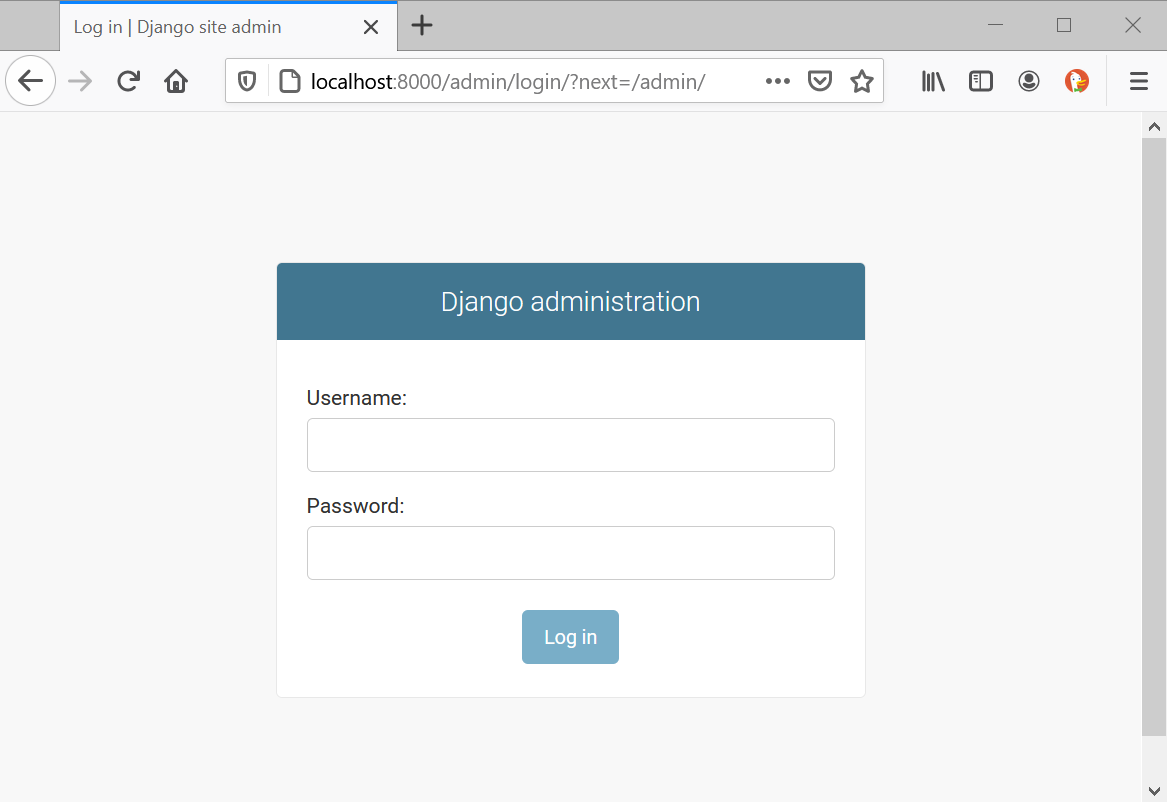
\includegraphics[width=2.5truein]{images/django/django-site-admin.png}
\caption{}
\centering
\end{figure}

\begin{figure}[h]{}
\centering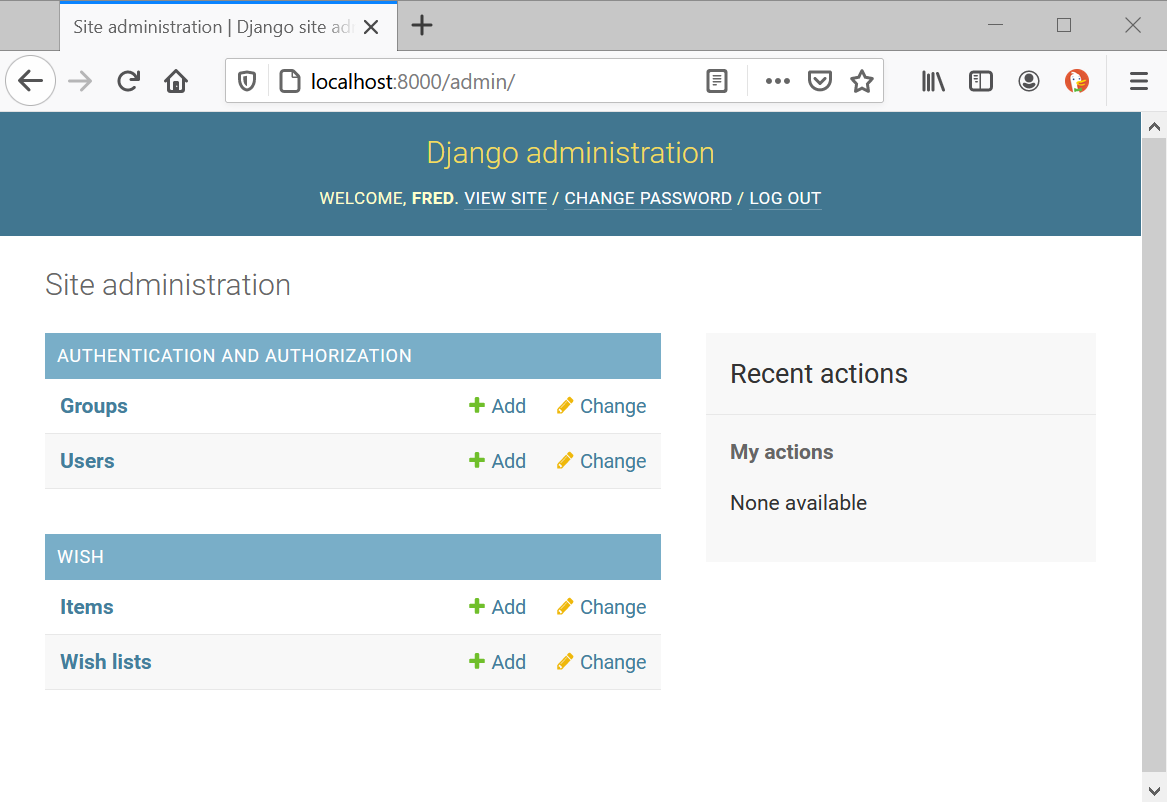
\includegraphics[width=2.5truein]{images/django/django-site-admin-after-connection.png}
\caption{}
\centering
\end{figure}

\hypertarget{x-quelques-conseils-de-base}{\section{Quelques conseils de base}}
\begin{enumerate}

\item{Surchargez la méthode \texttt{\emph{str}(self)} pour chaque classe que vous aurez définie dans le modèle. Cela permettra de construire une représentation textuelle pour chaque instance de votre classe. Cette information sera utilisée un peu partout dans le code, et donnera une meilleure idée de ce que l’on manipule. En plus, cette méthode est également appelée lorsque l’administration historisera une action (et comme cette étape sera inaltérable, autant qu’elle soit fixée dans le début).}

\item{La méthode \texttt{get\_absolute\_url(self)} retourne l’URL à laquelle on peut accéder pour obtenir les détails d’une instance. Par exemple:}

\end{enumerate}


\begin{verbatim}
def get_absolute_url(self):
    return reverse('myapp.views.details', args=[self.id])
\end{verbatim}

\begin{enumerate}

\item{Les attributs \texttt{Meta}:}

\end{enumerate}


\begin{verbatim}
class Meta:
	ordering = ['-field1', 'field2']
	verbose_name = 'my class in singular'
	verbose_name_plural = 'my class when is in a list!'
\end{verbatim}

\begin{enumerate}

\item{Le titre:}

\begin{itemize}

\item Soit en modifiant le template de l’administration

\item Soit en ajoutant l’assignation suivante dans le fichier \texttt{urls.py}: \texttt{admin.site.site\_header \= \"SuperBook Secret Area}.

\end{itemize}

\item{Prefetch}

\end{enumerate}


\href{https://hackernoon.com/all-you-need-to-know-about-prefetching-in-django-f9068ebe1e60?gi=7da7b9d3ad64}{https://hackernoon.com/all-you-need-to-know-about-prefetching-in-django-f9068ebe1e60?gi=7da7b9d3ad64}


\href{https://medium.com/hakibenita/things-you-must-know-about-django-admin-as-your-app-gets-bigger-6be0b0ee9614}{https://medium.com/hakibenita/things-you-must-know-about-django-admin-as-your-app-gets-bigger-6be0b0ee9614}


En gros, le problème de l’admin est que si on fait des requêtes imbriquées, on va flinguer l’application et le chargement de la page.
La solution consiste à utiliser la propriété \texttt{list\_select\_related} de la classe d’Admin, afin d’appliquer une jointure par défaut et
et gagner en performances.


\hypertarget{x-admin.modeladmin}{\section{admin.ModelAdmin}}
La classe \texttt{admin.ModelAdmin} que l’on retrouvera principalement dans le fichier \texttt{admin.py} de chaque application contiendra la définition de ce que l’on souhaite faire avec nos données dans l’administration. Cette classe (et sa partie Meta)


\hypertarget{x-l’affichage}{\section{L’affichage}}
Comme l’interface d’administration fonctionne (en trèèèès) gros comme un CRUD auto-généré, on trouve par défaut la possibilité de :


\begin{enumerate}

\item{Créer de nouveaux éléments}

\item{Lister les éléments existants}

\item{Modifier des éléments existants}

\item{Supprimer un élément en particulier.}

\end{enumerate}


Les affichages sont donc de deux types: en liste et par élément.


Pour les affichages en liste, le plus simple consiste à jouer sur la propriété \texttt{list\_display}.


Par défaut, la première colonne va accueillir le lien vers le formulaire d’édition.
On peut donc modifier ceci, voire créer de nouveaux liens vers d’autres éléments en construisant des URLs dynamiquement.


(Insérer ici l’exemple de Medplan pour les liens vers les postgradués :-))


Voir aussi comment personnaliser le fil d’Ariane ?


\hypertarget{x-les-filtres}{\section{Les filtres}}
\begin{enumerate}

\item{list\_filter}

\item{filter\_horizontal}

\item{filter\_vertical}

\item{date\_hierarchy}

\end{enumerate}


\hypertarget{x-les-permissions}{\section{Les permissions}}
On l’a dit plus haut, il vaut mieux éviter de proposer un accès à l’administration à vos utilisateurs.
Il est cependant possible de configurer des permissions spécifiques pour certains groupes, en leur autorisant certaines actions de visualisation/ajout/édition ou suppression.


Cela se joue au niveau du \texttt{ModelAdmin}, en implémentant les méthodes suivantes:


\begin{verbatim}
def has_add_permission(self, request):
	return True

def has_delete_permission(self, request):
	return True

def has_change_permission(self, request):
	return True
\end{verbatim}

On peut accéder aux informations de l’utilisateur actuellement connecté au travers de l’objet \texttt{request.user}.


\begin{enumerate}

\item{NOTE: ajouter un ou deux screenshots :-)}

\end{enumerate}


\hypertarget{x-les-relations}{\section{Les relations}}
\hypertarget{x-les-relations-1-n}{\subsection{Les relations 1-n}}
Les relations 1-n sont implémentées au travers de formsets (que l’on a normalement déjà décrits plus haut). L’administration permet de les définir d’une manière extrêmement simple, grâce à quelques propriétés.


L’implémentation consiste tout d’abord à définir le comportement du type d’objet référencé (la relation -N), puis à inclure cette définition au niveau du type d’objet référençant (la relation 1-).


\begin{verbatim}
class WishInline(TabularInline):
	model = Wish


class Wishlist(admin.ModelAdmin):
	...
	inlines = [WishInline]
	...
\end{verbatim}

Et voilà : l’administration d’une liste de souhaits (\emph{Wishlist}) pourra directement gérer des relations multiples vers des souhaits.


\hypertarget{x-les-auto-suggestions-et-auto-complétions}{\subsection{Les auto-suggestions et auto-complétions}}
Parler de l’intégration de select2.


\hypertarget{x-la-présentation}{\section{La présentation}}
Parler ici des \texttt{fieldsets} et montrer comment on peut regrouper des champs dans des groupes, ajouter un peu de javascript, …​


\hypertarget{x-les-actions-sur-des-sélections}{\section{Les actions sur des sélections}}
Les actions permettent de partir d’une liste d’éléments, et autorisent un utilisateur à appliquer une action sur une sélection d’éléments. Par défaut, il existe déjà une action de \textbf{suppression}.


Les paramètres d’entrée sont :


\begin{enumerate}

\item{L’instance de classe}

\item{La requête entrante}

\item{Le queryset correspondant à la sélection.}

\end{enumerate}


\begin{verbatim}
def double_quantity(self, request, queryset):
	for obj in queryset.all():
		obj.field += 1
		obj.save()
double_quantity.short_description = "Doubler la quantité des souhaits."
\end{verbatim}

Et pour informer l’utilisateur de ce qui a été réalisé, on peut aussi lui passer un petit message:


\begin{verbatim}
if rows_updated = 0:
	self.message_user(request, "Aucun élément n'a été impacté.")
else:
	self.message_user(request, "{} élément(s) mis à jour".format(rows_updated))
\end{verbatim}

\hypertarget{x-forms}{\chapter{Forms}}
Ou comment valider proprement des données entrantes.


\begin{figure}[h]{}
\centering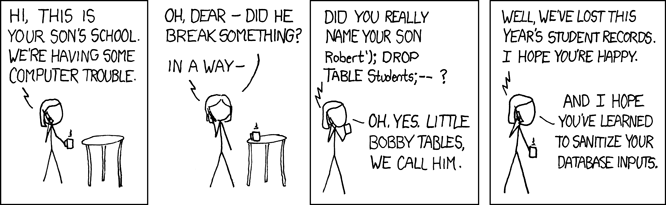
\includegraphics[width=2.5truein]{images/xkcd-327.png}


\end{figure}

Quand on parle de \texttt{forms}, on ne parle pas uniquement de formulaires Web. On pourrait considérer qu’il s’agit de leur objectif principal, mais on peut également voir un peu plus loin: on peut en fait voir les \texttt{forms} comme le point d’entrée pour chaque donnée arrivant dans notre application: il s’agit en quelque sorte d’un ensemble de règles complémentaires à celles déjà présentes au niveau du modèle.


L’exemple le plus simple est un fichier \texttt{.csv}: la lecture de ce fichier pourrait se faire de manière très simple, en récupérant les valeurs de chaque colonne et en l’introduisant dans une instance du modèle.


Mauvaise idée. On peut proposer trois versions d’un même code, de la version simple (lecture du fichier csv et jonglage avec les indices de colonnes), puis une version plus sophistiquée (et plus lisible, à base de \href{https://docs.python.org/3/library/csv.html#csv.DictReader}{DictReader}), et la version + à base de form.


Les données fournies par un utilisateur \textbf{doivent} \textbf{toujours} être validées avant introduction dans la base de données. Notre base de données étant accessible ici par l’ORM, la solution consiste à introduire une couche supplémentaire de validation.


Le flux à suivre est le suivant:


\begin{enumerate}

\item{Création d’une instance grâce à un dictionnaire}

\item{Validation des données et des informations reçues}

\item{Traitement, si la validation a réussi.}

\end{enumerate}


Ils jouent également deux rôles importants:


\begin{enumerate}

\item{Valider des données, en plus de celles déjà définies au niveau du modèle}

\item{Contrôler le rendu à appliquer aux champs.}

\end{enumerate}


Ils agissent come une glue entre l’utilisateur et la modélisation de vos structures de données.


\hypertarget{x-flux-de-validation}{\section{Flux de validation}}
| .Validation
| .is\_valid
| .clean\_fields
↓ .clean\_fields\_machin


\admonition{NOTE}{A compléter ;-)}
\hypertarget{x-dépendance-avec-le-modèle}{\section{Dépendance avec le modèle}}
Un \textbf{form} peut dépendre d’une autre classe Django. Pour cela, il suffit de fixer l’attribut \texttt{model} au niveau de la \texttt{class Meta} dans la définition.


\begin{verbatim}
from django import forms

from wish.models import Wishlist

class WishlistCreateForm(forms.ModelForm):
    class Meta:
        model = Wishlist
        fields = ('name', 'description')
\end{verbatim}

De cette manière, notre form dépendra automatiquement des champs déjà déclarés dans la classe \texttt{Wishlist}. Cela suit le principe de \texttt{DRY <don’t repeat yourself>`\_, et évite qu’une modification ne pourrisse le code: en testant les deux champs présent dans l’attribut fields}, nous pourrons nous assurer de faire évoluer le formulaire en fonction du modèle sur lequel il se base.


\hypertarget{x-rendu-et-affichage}{\section{Rendu et affichage}}
Le formulaire permet également de contrôler le rendu qui sera appliqué lors de la génération de la page. Si les champs dépendent du modèle sur lequel se base le formulaire, ces widgets doivent être initialisés dans l’attribut \texttt{Meta}. Sinon, ils peuvent l’être directement au niveau du champ.


\begin{verbatim}
from datetime import date

from django import forms

from .models import Accident


class AccidentForm(forms.ModelForm):
    class Meta:
        model = Accident
        fields = ('gymnast', 'educative', 'date', 'information')
        widgets = {
            'date' : forms.TextInput(
                     attrs={
                        'class' : 'form-control',
                        'data-provide' : 'datepicker',
                        'data-date-format' : 'dd/mm/yyyy',
                        'placeholder' : date.today().strftime("%d/%m/%Y")
                     }),
            'information' : forms.Textarea(
                            attrs={
                                'class' : 'form-control',
                                'placeholder' : 'Context (why, where, ...)'
                            })
        }
\end{verbatim}

\hypertarget{x-squelette-par-défaut}{\section{Squelette par défaut}}
On a d’un côté le form.as\_p, mais il y a beaucoup mieux que ça ;-) Voir les templates de Vitor et en passant par \texttt{widget-tweaks}.


\hypertarget{x-crispy-forms}{\section{Crispy-forms}}
Comme on l’a vu à l’instant, les forms, en Django, c’est le bien. Cela permet de valider des données reçues en entrée et d’afficher (très) facilement des formulaires à compléter par l’utilisateur.


Par contre, c’est lourd. Dès qu’on souhaite peaufiner un peu l’affichage, contrôler parfaitement ce que l’utilisateur doit remplir, modifier les types de contrôleurs, les placer au pixel près, …​ Tout ça demande énormément de temps. Et c’est là qu’intervient \href{http://django-crispy-forms.readthedocs.io/en/latest/}{Django-Crispy-Forms}. Cette librairie intègre plusieurs frameworks CSS (Bootstrap, Foundation et uni-form) et permet de contrôler entièrement le \textbf{layout} et la présentation.


(c/c depuis le lien ci-dessous)


Pour chaque champ, crispy-forms va :


\begin{itemize}

\item utiliser le \texttt{verbose\_name} comme label.

\item vérifier les paramètres \texttt et \texttt{null} pour savoir si le champ est obligatoire.

\item utiliser le type de champ pour définir le type de la balise \texttt{<input>}.

\item récupérer les valeurs du paramètre \texttt{choices} (si présent) pour la balise \texttt{<select>}.

\end{itemize}


\href{http://dotmobo.github.io/django-crispy-forms.html}{http://dotmobo.github.io/django-crispy-forms.html}


\hypertarget{x-en-conclusion}{\section{En conclusion}}
\begin{enumerate}

\item{Toute donnée entrée par l’utilisateur \textbf{doit} passer par une instance de \texttt{form}.}

\item{euh ?}

\end{enumerate}


\hypertarget{x-vues}{\chapter{Vues}}
Une vue correspond à un contrôleur dans le pattern MVC. Tout ce que vous pourrez définir au niveau du fichier \texttt{views.py} fera le lien entre le modèle stocké dans la base de données et ce avec quoi l’utilisateur pourra réellement interagir (le \texttt{template}).


Chaque vue peut etre représentée de deux manières: soit par des fonctions, soit par des classes. Le comportement leur est propre, mais le résultat reste identique. Le lien entre l’URL à laquelle l’utilisateur accède et son exécution est faite au travers du fichier \texttt{gwift/urls.py}, comme on le verra par la suite.


\hypertarget{x-function-based-views}{\section{Function Based Views}}
Les fonctions (ou \texttt{FBV} pour \textbf{Function Based Views}) permettent une implémentation classique des contrôleurs. Au fur et à mesure de votre implémentation, on se rendra compte qu’il y a beaucoup de répétitions dans ce type d’implémentation: elles ne sont pas obsolètes, mais dans certains cas, il sera préférable de passer par les classes.


Pour définir la liste des \texttt{WishLists}  actuellement disponibles, on précédera de la manière suivante:


\begin{enumerate}

\item{Définition d’une fonction qui va récupérer les objets de type \texttt{WishList} dans notre base de données. La valeur de retour sera la construction d’un dictionnaire (le \textbf{contexte}) qui sera passé à un template HTML. On démandera à ce template d’effectuer le rendu au travers de la fonction \texttt{render}, qui est importée par défaut dans le fichier \texttt{views.py}.}

\item{Construction d’une URL qui permettra de lier l’adresse à l’exécution de la fonction.}

\item{Définition du squelette.}

\end{enumerate}


\begin{verbatim}
# wish/views.py

from django.shortcuts import render
from .models import Wishlist

def wishlists(request):
	wishlists = Wishlist.objects.all()
	return render(
		request,
		'wish/list.html',
		{
			'wishlists': wishlists
		}
	)
\end{verbatim}

Rien qu’ici, on doit déjà tester deux choses:


\begin{enumerate}

\item{Qu’on construit bien le modèle attendu - la liste de tous les souhaits déjà émis.}

\item{Que le template \texttt{wish/list.html} existe bien - sans quoi, on va tomber sur une erreur de type \texttt{TemplateDoesNotExist} dans notre environnement de test, et sur une erreur 500 en production.}

\end{enumerate}


A ce stade, vérifiez que la variable \texttt{TEMPLATES} est correctement initialisée dans le fichier \texttt{gwift/settings.py} et que le fichier \texttt{templates/wish/list.html} ressemble à ceci:


\begin{verbatim}
<!doctype html>
<html>
	<head>
		<meta charset="utf-8">
		<meta http-equiv="x-ua-compatible" content="ie=edge">
		<title></title>
	</head>
	<body>
		<p>Mes listes de souhaits</p>
		<ul>
		
			<li>glossterm::[ wishlist.name ]: glossterm::[ wishlist.description ]</li>
		
		</ul>
	</body>
</html>
\end{verbatim}

A présent, ajoutez quelques listes de souhaits grâce à un \textbf{shell}, puis lancez le serveur:


\begin{verbatim}
$ python manage.py shell
>>> from wish.models import Wishlist
>>> Wishlist.create('Décembre', "Ma liste pour les fêtes de fin d'année")
<Wishlist: Wishlist object>
>>> Wishlist.create('Anniv 30 ans', "Je suis vieux! Faites des dons!")
<Wishlist: Wishlist object>
\end{verbatim}

Lancez le serveur grâce à la commande \texttt{python manage.py runserver}, ouvrez un navigateur quelconque et rendez-vous à l’adresse `http://localhost:8000 <\href{http://localhost:8000>`}{http://localhost:8000>`}. Vous devriez obtenir le résultat suivant:


\begin{enumerate}

\item{image:: mvc/my-first-wishlists.png
:align: center}

\end{enumerate}


Rien de très sexy, aucune interaction avec l’utilisateur, très peu d’utilisation des variables contextuelles, mais c’est un bon début! =)


\hypertarget{x-class-based-views}{\section{Class Based Views}}
Les classes, de leur côté, implémente le \textbf{pattern} objet et permettent d’arriver facilement à un résultat en très peu de temps, parfois même en définissant simplement quelques attributs, et rien d’autre. Pour l’exemple, on va définir deux classes qui donnent exactement le même résultat que la fonction \texttt{wishlists} ci-dessus. Une première fois en utilisant une classe générique vierge, et ensuite en utilisant une classe de type \texttt{ListView}.


Voir \href{https://ccbv.co.uk/}{Classy Class Based Views}.


L’idée derrière les classes est de définir des fonctions \textbf{par convention plutôt que par configuration}.


\admonition{NOTE}{à compléter ici :-)}
\hypertarget{x-listview}{\subsection{ListView}}
Les classes génériques implémentent un aspect bien particulier de la représentation d’un modèle, en utilisant très peu d’attributs. Les principales classes génériques sont de type \texttt{ListView}, […​]. L’implémentation consiste, exactement comme pour les fonctions, à:


\begin{enumerate}

\item{Définir une sous-classe de celle que l’on souhaite utiliser}

\item{Câbler l’URL qui lui sera associée}

\item{Définir le squelette.}

\end{enumerate}


\begin{verbatim}
# wish/views.py

from django.views.generic import ListView

from .models import Wishlist

class WishListList(ListView):
	context_object_name = 'wishlists'
	model = Wishlist
	template_name = 'wish/list.html'
\end{verbatim}

Il est même possible de réduire encore ce morceau de code en définissant juste le snippet suivant :


\begin{verbatim}
# wish/views.py

from django.views.generic import ListView

from .models import Wishlist

class WishListList(ListView):
	context_object_name = 'wishlists'
\end{verbatim}

Par inférence, Django construit beaucoup d’informations: si on n’avait pas spécifié les variables \texttt{context\_object\_name} et \texttt{template\_name}, celles-ci auraient pris les valeurs suivantes:


\begin{itemize}

\item \texttt{context\_object\_name}: \texttt{wishlist\_list} (ou plus précisément, le nom du modèle suivi de \texttt{\_list})

\item \texttt{template\_name}: \texttt{wish/wishlist\_list.html} (à nouveau, le fichier généré est préfixé du nom du modèle).

\end{itemize}


En l’état, par rapport à notre précédente vue basée sur une fonction, on y gagne sur les conventions utilisées et le nombre de tests à réaliser. A vous de voir la déclaration que vous préférez, en fonction de vos affinités et du résultat que vous souhaitez atteindre.


\admonition{NOTE}{un petit tableau de différence entre les deux ? :-)}
\begin{verbatim}
# gwift/urls.py

from django.conf.urls import include, url
from django.contrib import admin

from wish.views import WishListList

urlpatterns = [
	url(r'^admin/', include(admin.site.urls)),
	url(r'^$', WishListList.as_view(), name='wishlists'),
]
\end{verbatim}

C’est tout. Lancez le serveur, le résultat sera identique.


\hypertarget{x-templates}{\chapter{Templates}}
Avant de commencer à interagir avec nos données au travers de listes, formulaires et d’interfaces sophistiquées, quelques mots sur les templates: il s’agit en fait de \textbf{squelettes} de présentation, recevant en entrée un dictionnaire contenant des clés-valeurs et ayant pour but de les afficher selon le format que vous définirez.


En intégrant un ensemble de \textbf{tags}, cela vous permettra de greffer les données reçues en entrée dans un patron prédéfini.


\admonition{NOTE}{(je ne sais plus ce que je voulais dire ici)}
Un squelette de page HTML basique ressemble à ceci:


\begin{verbatim}
<!doctype html>
<html>
    <head>
        <meta charset="utf-8">
        <meta http-equiv="x-ua-compatible" content="ie=edge">
        <title></title>
    </head>
    <body>
        <p>Hello world!</p>
    </body>
</html>
\end{verbatim}

Notre première vue permettra de récupérer la liste des objets de type \texttt{Wishlist} que nous avons définis dans le fichier \texttt{wish/models.py}. Supposez que cette liste soit accessible \textbf{via} la clé \texttt{wishlists} d’un dictionnaire passé au template. Elle devient dès lors accessible grâce aux tags

De même, il sera possible d’accéder aux propriétés de cette objet de la même manière: \texttt{wishlist.id}, \texttt{wishlist.description}, ... et d’ainsi respecter la mise en page que nous souhaitons.


En reprenant l’exemple de la page HTML définie ci-dessus, on pourra l’agrémenter de la manière suivante:


\begin{verbatim}
<!doctype html>
<html>
    <head>
        <meta charset="utf-8">
        <meta http-equiv="x-ua-compatible" content="ie=edge">
        <title></title>
    </head>
    <body>
        <p>Mes listes de souhaits</p>
        <ul>
        
            <li>glossterm::[ wishlist.name ]: glossterm::[ wishlist.description ]</li>
        
        </ul>
    </body>
</html>
\end{verbatim}

\begin{figure}[h]{}
\centering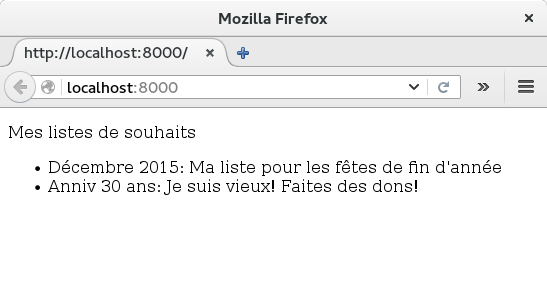
\includegraphics[width=2.5truein]{images/html/my-first-wishlists.png}


\end{figure}

Mais plutôt que de réécrire à chaque fois le même entête, on peut se simplifier la vie en implémentant un héritage au niveau des templates. Pour cela, il suffit de définir des blocs de contenu, et d'\textbf{étendre} une page de base, puis de surcharger ces mêmes blocs.


Par exemple, si on repart de notre page de base ci-dessus, on va y définir deux blocs réutilisables:


\begin{verbatim}
<!-- templates/base.html -->

<!doctype html>
<html>
    <head>
        <meta charset="utf-8">
        <meta http-equiv="x-ua-compatible" content="ie=edge">
        <title>Gwift</title> 
    </head>
    <body>
        <p>Hello world!</p> 
    </body>
</html>
\end{verbatim}


La page HTML pour nos listes de souhaits devient alors:


\begin{verbatim}
<!-- templates/wishlist/wishlist_list.html -->

 

glossterm::[ block.super ] - Listes de souhaits 

 
<p>Mes listes de souhaits</p>
<ul>

    <li>glossterm::[ wishlist.name ]: glossterm::[ wishlist.description ]</li>

</ul>
\end{verbatim}


\hypertarget{x-structure-et-configuration}{\section{Structure et configuration}}
Il est conseillé que les templates respectent la structure de vos différentes applications, mais dans un répertoire à part. Par convention, nous les placerons dans un répertoire \texttt{templates}. La hiérarchie des fichiers devient alors celle-ci:


\begin{verbatim}
$ tree templates/
templates/
└── wish
    └── list.html
\end{verbatim}

Par défaut, Django cherchera les templates dans les répertoirer d’installation. Vous devrez vous éditer le fichier \texttt{gwift/settings.py} et ajouter, dans la variable \texttt{TEMPLATES}, la clé \texttt{DIRS} de la manière suivante:


\begin{verbatim}
TEMPLATES = [
    {
        ...
        'DIRS': [ 'templates' ],
        ...
    },
]
\end{verbatim}

\hypertarget{x-builtins}{\section{Builtins}}
Django vient avec un ensemble de \textbf{tags} ou \textbf{template tags}. On a vu la boucle \texttt{for} ci-dessus, mais il existe \href{https://docs.djangoproject.com/fr/1.9/ref/templates/builtins/}{beaucoup d’autres tags nativement présents}. Les principaux sont par exemple:


\begin{itemize}

\item if, conditions, etc. permet de vérifier une condition et de n’afficher le contenu du bloc que si la condition est vérifiée.

\item Opérateurs de comparaison (gueules de loups, in, not in, etc.)

\item Regroupements avec le tag regroup by ... as 

\item url pour construire facilement une URL à partir de son nom

\item urlize qui permet de remplacer des URLs trouvées dans un champ CharField ou TextField en lien cliquable

\end{itemize}


Chacune de ces fonctions peut être utilisée autant au niveau des templates qu’au niveau du code. Il suffit d’aller les chercher dans le package \texttt{django.template.defaultfilters}. Par exemple:


\begin{verbatim}
from django.db import models
from django.template.defaultfilters import urlize


class Suggestion(models.Model):
    """Représentation des suggestions.
    """
    subject = models.TextField(verbose_name="Sujet")

    def urlized_subject(self):
        """
        Voir https://docs.djangoproject.com/fr/3.0/howto/custom-template-tags/
        """
        return urlize(self.subject, autoescape=True)
\end{verbatim}

\hypertarget{x-non-builtins}{\section{Non-builtins}}
En plus des quelques tags survolés ci-dessus, il est également possible de construire ses propres tags. La structure est un peu bizarre, car elle consiste à ajouter un paquet dans une de vos applications, à y définir un nouveau module et à y définir un ensemble de fonctions. Chacune de ces fonctions correspondra à un tag appelable depuis vos templates.


Il existe trois types de tags \textbf{non-builtins}:


\begin{enumerate}

\item \textbf{Les filtres} - on peut les appeler grâce au \textbf{pipe} directement après une valeur dans le template.

\item \textbf{Les tags simples} - ils peuvent prendre une valeur ou plusieurs en paramètre et retourne une nouvelle valeur. Pour les appeler, c’est \textbf{via} les tags nom de la fonction param1 param2...

\item \textbf{Les tags d inclusion}: ils retournent un contexte (ie. un dictionnaire), qui est ensuite passé à un nouveau template. Type include.

\end{enumerate}


Pour l’implémentation:


\begin{enumerate}

\item On prend l’application \texttt{wish} et on y ajoute un répertoire \texttt{templatetags}, ainsi qu’un fichier \texttt{init.py}.

\item{Dans ce nouveau paquet, on ajoute un nouveau module que l’on va appeler \texttt{tools.py}}

\item{Dans ce module, pour avoir un aperçu des possibilités, on va définir trois fonctions (une pour chaque type de tags possible).}

\end{enumerate}


\begin{verbatim}
[Inclure un tree du dossier template tags]
\end{verbatim}

\hypertarget{x-filtres}{\subsection{Filtres}}
\begin{verbatim}
# wish/tools.py

from django import template

from wish.models import Wishlist

register = template.Library()

@register.filter(is_safe=True)
def add_xx(value):
    return '%sxx' % value
\end{verbatim}

\hypertarget{x-tags-simples}{\subsection{Tags simples}}
\begin{verbatim}
# wish/tools.py

from django import template

from wish.models import Wishlist


register = template.Library()


@register.simple_tag
def current_time(format_string):
    return datetime.datetime.now().strftime(format_string)
\end{verbatim}

\hypertarget{x-tags-d’inclusion}{\subsection{Tags d’inclusion}}
\begin{verbatim}
# wish/tools.py

from django import template

from wish.models import Wishlist


register = template.Library()


@register.inclusion_tag('wish/templatetags/wishlists_list.html')
def wishlists_list():
    return { 'list': Wishlist.objects.all() }
\end{verbatim}

\hypertarget{x-contexts-processors}{\section{Contexts Processors}}
Un \texttt{context processor} permet d’ajouter des informations par défaut à un contexte (le dictionnaire qu’on passe de la vue au template).
L’idée est d’ajouter une fonction à un module Python à notre projet, puis de le référencer parmi
  les CONTEXT\_PROCESSORS de nos paramètres généraux. Cette fonction doit peupler un dictionnaire, et les clés de ce dictionnaire seront
  directement ajoutées à tout autre dictionnaire/contexte passé à une vue. Par exemple:


(cf. \href{https://stackoverflow.com/questions/60515797/default-context-for-all-pages-django}{StackOverflow} - à retravailler)


\begin{verbatim}
from product.models import SubCategory, Category


def add_variable_to_context(request):
    return {
        'subCategories': SubCategory.objects.order_by('id').all(),
        'categories': Category.objects.order_by("id").all(),
    }
\end{verbatim}

\begin{verbatim}
'OPTIONS': {
    'context_processors': [
        ....
        'core.context_processors.add_variable_to_context',
        ....
    ],
},
\end{verbatim}

\hypertarget{x-mise-en-page}{\section{Mise en page}}
Pour que nos pages soient un peu plus \textbf{eye-candy} que ce qu’on a présenté ci-dessus, nous allons modifié notre squelette pour qu’il se base sur \href{http://getbootstrap.com/>`}{http://getbootstrap.com/>`}. Nous placerons une barre de navigation principale, la possibilité de se connecter pour l’utilisateur et définirons quelques emplacements à utiliser par la suite. Reprenez votre fichier base.html et modifiez le comme ceci:


\begin{verbatim}


<!DOCTYPE html>
<!--[if IE 9]><html class="lt-ie10" lang="en" > <![endif]-->
<html class="no-js" lang="en">

<head>
    <meta charset="utf-8">
    <meta name="viewport" content="width=device-width, initial-scale=1.0">
    <link href="//maxcdn.bootstrapcdn.com/bootstrap/3.3.6/css/bootstrap.min.css" rel="stylesheet">
    <script src="//code.jquery.com/jquery.min.js"></script>
    <script src="//maxcdn.bootstrapcdn.com/bootstrap/3.3.6/js/bootstrap.min.js"></script>
    <link href='https://fonts.googleapis.com/css?family=Open+Sans' rel='stylesheet' type='text/css'>
    <link rel="stylesheet" href="https://maxcdn.bootstrapcdn.com/font-awesome/4.4.0/css/font-awesome.min.css">
    <link href="" rel="stylesheet">
    <link rel="icon" href="" />
    <title>Gwift</title>
</head>

<body class="base-body">

    <!-- navigation -->
    <div class="nav-wrapper">
        <div id="nav">
            <nav class="navbar navbar-default navbar-static-top navbar-shadow">
                <div class="container-fluid">
                    <div class="navbar-header">
                        <button type="button" class="navbar-toggle" data-toggle="collapse" data-target="#menuNavbar">
                            <span class="icon-bar"></span>
                            <span class="icon-bar"></span>
                            <span class="icon-bar"></span>
                        </button>
                        <a class="navbar-brand" href="/">
                            <img src="" />
                        </a>
                    </div>
                    <div class="collapse navbar-collapse" id="menuNavbar">
                        
                    </div>
                </div>
            </nav>
        </div>
    </div>
    <!-- end navigation -->

    <!-- content -->
    <div class="container">
        <div class="row">
            <div class="col-md-8">
                
            </div>
        </div>
    </div>
    <!-- end content -->

    <!-- footer -->
    <footer class="footer">
        
    </footer>
    <!-- end footer -->
</body>
</html>
\end{verbatim}

Quelques remarques:


\begin{itemize}

\item La première ligne du fichier inclut le \textbf{tag}  load staticfiles On y reviendra par la suite, mais en gros, cela permet de faciliter la gestion des fichiers statiques, notamment en les appelent grâce à la commande static 'img/header.png' ou static 'css/app\_style.css' .

\item La balise \texttt{<head />} est bourée d’appel vers des ressources stockées sur des CDN.

\item Les balises permettent de faire hériter du contenu depuis une autre page. On l’utilise notamment dans notre page \texttt{templates/wish/list.html}.

\item Pour l’entête et le bas de page n fait appel aux balises include pour charger un nom de fichier - ces fichiers sont des fichiers physiques, placés sur le filesystem, juste à côté du fichier . De façon bête et méchante, cela inclut juste du contenu HTML. Le contenu des fichiers  et  est copié ci-dessous.

\end{itemize}


\begin{verbatim}
<!-- gwift/templates/wish/list.html -->




    <p>Mes listes de souhaits</p>
    <ul>
    
        <li>glossterm::[ wishlist.name ]: glossterm::[ wishlist.description ]</li>
    
    </ul>

\end{verbatim}

\begin{verbatim}
<!-- gwift/templates/_menu_items.html -->
<ul class="nav navbar-nav">
    <li class="">
        <a href="#">
            <i class="fa fa-calendar"></i> Mes listes
        </a>
    </li>
</ul>
<ul class="nav navbar-nav navbar-right">
    <li class="">
        <a href="#">
            <i class="fa fa-user"></i> Login / Register
        </a>
    </li>
</ul>
\end{verbatim}

\begin{verbatim}
<!-- gwift/templates/_footer.html -->
<div class="container">
    Copylefted '16
</div>
\end{verbatim}

En fonction de vos affinités, vous pourriez passer par PluCSS, KNACSS, Cascade, PureCSS, Semantic-UI, ... 
Pour notre plus grand bonheur, les frameworks de ce type pullulent.
Reste à choisir le bon.

\textbf{A priori}, si vous relancez le serveur de développement maintenant, vous devriez déjà voir les modifications…​ Mais pas les images, ni tout autre fichier statique.


\hypertarget{x-fichiers-statiques}{\subsection{Fichiers statiques}}
Si vous ouvrez la page et que vous lancez la console de développement (F12, sur la majorité des navigateurs), vous vous rendrez compte que certains fichiers ne sont pas disponibles. Il s’agit des fichiers suivants:


\begin{itemize}

\item \texttt{/static/css/style.css}

\item \texttt{/static/img/favicon.ico}

\item \texttt{/static/img/gwift-20x20.png}.

\end{itemize}


En fait, par défaut, les fichiers statiques sont récupérés grâce à deux handlers:


\begin{enumerate}

\item{\texttt{django.contrib.staticfiles.finders.FileSystemFinder} et . \texttt{django.contrib.staticfiles.finders.AppDirectoriesFinder}.}

\end{enumerate}


En fait, Django va considérer un répertoire \texttt{static} à l’intérieur de chaque application. Si deux fichiers portent le même nom, le premier trouvé sera pris. Par facilité, et pour notre développement, nous placerons les fichiers statiques dans le répertoire \texttt{gwift/static}. On y trouve donc:


\begin{verbatim}
[inclure un tree du répertoire gwift/static]
\end{verbatim}

\begin{verbatim}
# gwift/settings/base.py

STATIC_URL = '/static/'
\end{verbatim}

\begin{verbatim}
# gwift/settings/dev.py

STATICFILES_DIRS = [
    os.path.join(BASE_DIR, "static"),
]
\end{verbatim}

En production par contre, nous ferons en sorte que le contenu statique soit pris en charge par le front-end Web (Nginx), raison pour laquelle cette variable n’est initialisée que dans le fichier des paramètres liés au développement.


Au final, cela ressemble à ceci:


\begin{enumerate}

\item{image:: mvc/my-first-wishlists.png
:align: center}

\end{enumerate}


\hypertarget{x-urls-et-espaces-de-noms}{\chapter{URLs et espaces de noms}}
La gestion des URLs permet \textbf{grosso modo} d’assigner une adresse paramétrée ou non à une fonction Python. La manière simple consiste à modifier le fichier \texttt{gwift/settings.py} pour y ajouter nos correspondances. Par défaut, le fichier ressemble à ceci:


\begin{verbatim}
# gwift/urls.py

from django.conf.urls import include, url
from django.contrib import admin

urlpatterns = [
    url(r'^admin/', include(admin.site.urls)),
]
\end{verbatim}

La variable \texttt{urlpatterns} associe un ensemble d’adresses à des fonctions. Dans le fichier \textbf{nu}, seul le \textbf{pattern} \texttt{admin} est défini, et inclut toutes les adresses qui sont définies dans le fichier \texttt{admin.site.urls}.


\admonition{NOTE}{petit mot d’explication sur les expressions rationnelles.}
\begin{verbatim}
# admin.site.urls.py
\end{verbatim}

Pour reprendre l’exemple où on en était resté:


\begin{verbatim}
# gwift/urls.py

from django.conf.urls import include, url
from django.contrib import admin

from wish import views as wish_views

urlpatterns = [
	url(r'^admin/', include(admin.site.urls)),
	url(r'^$', wish_views.wishlists, name='wishlists'),
]
\end{verbatim}

A présent, on doit tester que l’URL racine de notre application mène bien vers la fonction \texttt{wish\_views.wishlists}.


Prenons par exemple l’exemple de Twitter : quand on accède à une URL, elle est de la forme \texttt{https://twitter.com/<user>`}. Sauf que les pages \texttt{about} et \texttt{help} existent également. Pour implémenter ce type de précédence, il faudrait implémenter les URLs de la manière suivante:


\begin{verbatim}
| about
| help
| <user>
\end{verbatim}

Mais cela signifie aussi que les utilisateurs \texttt{about} et \texttt{help} (s’ils existent…​) ne pourront jamais accéder à leur profil. Une dernière solution serait de maintenir une liste d’authorité des noms d’utilisateur qu’il n’est pas possible d’utiliser.


D’où l’importance de bien définir la séquence de déinition de ces routes, ainsi que des espaces de noms.


L’idée des espaces de noms ou \emph{namespaces} est de définir un \emph{sous-répertoire} dans lequel on trouvera nos nouvelles routes. Cette manière de procéder permet notamment de répondre au problème ci-dessous, en définissant un sous-dossier type \texttt{https://twitter.com/users/<user>`}.


De là, découle une autre bonne pratique: l’utilisation de \emph{breadcrumbs} (\href{https://stackoverflow.com/questions/826889/how-to-implement-breadcrumbs-in-a-django-template}{https://stackoverflow.com/questions/826889/how-to-implement-breadcrumbs-in-a-django-template}) ou de guidelines de navigation.


\hypertarget{x-reverse}{\section{Reverse}}
En associant un nom ou un libellé à chaque URL, il est possible de récupérer sa \textbf{traduction}. Cela implique par contre de ne plus toucher à ce libellé par la suite…​


Dans le fichier \texttt{urls.py}, on associe le libellé \texttt{wishlists} à l’URL \$ (c’est-à-dire la racine du site):


\begin{verbatim}
from wish.views import WishListList

urlpatterns = [
    url(r'^admin/', include(admin.site.urls)),
    url(r'^$', WishListList.as_view(), name='wishlists'),
]
\end{verbatim}

De cette manière, dans nos templates, on peut à présent construire un lien vers la racine avec le tags suivant:


\begin{verbatim}
<a href="">glossterm::[ yearvar ] Archive</a>
\end{verbatim}

De la même manière, on peut également récupérer l’URL de destination pour n’importe quel libellé, de la manière suivante:


\begin{verbatim}
from django.core.urlresolvers import reverse_lazy

wishlists_url = reverse_lazy('wishlists')
\end{verbatim}

\hypertarget{x-authentification}{\chapter{Authentification}}
Comme on l’a vu dans la partie sur le modèle, nous souhaitons que le créateur d’une liste puisse retrouver facilement les éléments qu’il aura créé. Ce dont nous n’avons pas parlé cependant, c’est la manière dont l’utilisateur va pouvoir créer son compte et s’authentifier. La \href{https://docs.djangoproject.com/en/stable/topics/auth/}{documentation} est très complète, nous allons essayer de la simplifier au maximum. Accrochez-vous, le sujet peut être complexe.


\hypertarget{x-mécanisme-d’authentification}{\section{Mécanisme d’authentification}}
On peut schématiser le flux d’authentification de la manière suivante :


En gros:


\begin{enumerate}

\item{La personne accède à une URL qui est protégée (voir les décorateurs \@login\_required et le mixin LoginRequiredMixin)}

\item{Le framework détecte qu’il est nécessaire pour la personne de se connecter (grâce à un paramètre type LOGIN\_URL)}

\item{Le framework présente une page de connexion ou un mécanisme d’accès pour la personne (template à définir)}

\item{Le framework récupère les informations du formulaire, et les transmets aux différents backends d’authentification, dans l’ordre}

\item{Chaque backend va appliquer la méthode \texttt{authenticate} en cascade, jusqu’à ce qu’un backend réponde True ou qu’aucun ne réponde}

\item{La réponse de la méthode authenticate doit être une instance d’un utilisateur, tel que définit parmi les paramètres généraux de l’application.}

\end{enumerate}


En résumé (bis):


\begin{enumerate}

\item{Une personne souhaite se connecter;}

\item{Les backends d’authentification s’enchaîne jusqu’à trouver une bonne correspondance. Si aucune correspondance n’est trouvée, on envoie la personne sur les roses.}

\item{Si OK, on retourne une instance de type current\_user, qui pourra être utilisée de manière uniforme dans l’application.}

\end{enumerate}


Ci-dessous, on définit deux backends différents pour mieux comprendre les différentes possibilités:


\begin{enumerate}

\item{Une authentification par jeton}

\item{Une authentification LDAP}

\end{enumerate}


\begin{verbatim}
from datetime import datetime

from django.contrib.auth import backends, get_user_model
from django.db.models import Q

from accounts.models import Token  


UserModel = get_user_model()


class TokenBackend(backends.ModelBackend):
    def authenticate(self, request, username=None, password=None, **kwargs):
        """Authentifie l'utilisateur sur base d'un jeton qu'il a reçu.

        On regarde la date de validité de chaque jeton avant d'autoriser l'accès.
        """
        token = kwargs.get("token", None)

        current_token = Token.objects.filter(token=token, validity_date__gte=datetime.now()).first()

        if current_token:
            user = current_token.user

            current_token.last_used_date = datetime.now()
            current_token.save()

            return user

        return None
\end{verbatim}


\begin{verbatim}
from django.contrib.auth import backends, get_user_model

from ldap3 import Server, Connection, ALL
from ldap3.core.exceptions import LDAPPasswordIsMandatoryError

from config import settings


UserModel = get_user_model()


class LdapBackend(backends.ModelBackend):
    """Implémentation du backend LDAP pour la connexion des utilisateurs à l'Active Directory.
    """
    def authenticate(self, request, username=None, password=None, **kwargs):
        """Authentifie l'utilisateur au travers du serveur LDAP.
        """

        ldap_server = Server(settings.LDAP_SERVER, get_info=ALL)
        ldap_connection = Connection(ldap_server, user=username, password=password)

        try:
            if not ldap_connection.bind():
                raise ValueError("Login ou mot de passe incorrect")
        except (LDAPPasswordIsMandatoryError, ValueError) as ldap_exception:
            raise ldap_exception

        user, _ = UserModel.objects.get_or_create(username=username)
\end{verbatim}

On peut résumer le mécanisme d’authentification de la manière suivante:


\begin{itemize}

\item Si vous voulez modifier les informations liées à un utilisateur, orientez-vous vers la modification du modèle. Comme nous le verrons ci-dessous, il existe trois manières de prendre ces modifications en compte. Voir également \href{https://docs.djangoproject.com/en/stable/topics/auth/customizing/}{ici}.

\item Si vous souhaitez modifier la manière dont l’utilisateur se connecte, alors vous devrez modifier le.

\end{itemize}


\hypertarget{x-modification-du-modèle}{\section{Modification du modèle}}
Dans un premier temps, Django a besoin de manipuler \href{https://docs.djangoproject.com/en/1.9/ref/contrib/auth/#user-model}{des instances de type \texttt{django.contrib.auth.User}}. Cette classe implémente les champs suivants:


\begin{itemize}

\item \texttt{username}

\item \texttt{first\_name}

\item \texttt{last\_name}

\item textttjaguarondi27@gmail.com

\item \texttt{password}

\item \texttt{date\_joined}.

\end{itemize}


D’autres champs, comme les groupes auxquels l’utilisateur est associé, ses permissions, savoir s’il est un super-utilisateur, …​ sont moins pertinents pour le moment. Avec les quelques champs déjà définis ci-dessus, nous avons de quoi identifier correctement nos utilisateurs. Inutile d’implémenter nos propres classes, puisqu’elles existent déjà :-)


Si vous souhaitez ajouter un champ, il existe trois manières de faire.


\hypertarget{x-extension-du-modèle-existant}{\section{Extension du modèle existant}}
Le plus simple consiste à créer une nouvelle classe, et à faire un lien de type \texttt{OneToOne} vers la classe \texttt{django.contrib.auth.User}. De cette manière, on ne modifie rien à la manière dont Django authentife ses utlisateurs: tout ce qu’on fait, c’est un lien vers une table nouvellement créée, comme on l’a déjà vu au point […​voir l’héritage de modèle]. L’avantage de cette méthode, c’est qu’elle est extrêmement flexible, et qu’on garde les mécanismes Django standard. Le désavantage, c’est que pour avoir toutes les informations de notre utilisateur, on sera obligé d’effectuer une jointure sur le base de données, ce qui pourrait avoir des conséquences sur les performances.


\hypertarget{x-substitution}{\section{Substitution}}
Avant de commencer, sachez que cette étape doit être effectuée \textbf{avant la première migration}. Le plus simple sera de définir une nouvelle classe héritant de \texttt{django.contrib.auth.User} et de spécifier la classe à utiliser dans votre fichier de paramètres. Si ce paramètre est modifié après que la première migration ait été effectuée, il ne sera pas pris en compte. Tenez-en compte au moment de modéliser votre application.


\begin{verbatim}
AUTH_USER_MODEL = 'myapp.MyUser'
\end{verbatim}

Notez bien qu’il ne faut pas spécifier le package \texttt{.models} dans cette injection de dépendances: le schéma à indiquer est bien \texttt{<nom de l’application>.<nom de la classe>}.


\hypertarget{x-backend}{\subsection{Backend}}

\hypertarget{x-templates}{\subsection{Templates}}
Ce qui n’existe pas par contre, ce sont les vues. Django propose donc tout le mécanisme de gestion des utilisateurs, excepté le visuel (hors administration). En premier lieu, ces paramètres sont fixés dans le fichier `settings <\href{https://docs.djangoproject.com/en/1.8/ref/settings/auth}. On y trouve par exemple les paramètres suivants:


\begin{itemize}

\item \texttt{LOGIN\_REDIRECT\_URL}: si vous ne spécifiez pas le paramètre \texttt{next}, l’utilisateur sera automatiquement redirigé vers cette page.

\item \texttt{LOGIN\_URL}: l’URL de connexion à utiliser. Par défaut, l’utilisateur doit se rendre sur la page \texttt{/accounts/login}.

\end{itemize}


\hypertarget{x-social-authentification}{\subsection{Social-Authentification}}
Voir ici : \href{https://github.com/omab/python-social-auth}{python social auth}


\hypertarget{x-un-petit-mot-sur-oauth}{\subsection{Un petit mot sur OAuth}}
OAuth est un standard libre définissant un ensemble de méthodes à implémenter pour l’accès (l’autorisation) à une API. Son fonctionnement se base sur un système de jetons (Tokens), attribués par le possesseur de la ressource à laquelle un utilisateur souhaite accéder.


Le client initie la connexion en demandant un jeton au serveur. Ce jeton est ensuite utilisée tout au long de la connexion, pour accéder aux différentes ressources offertes par ce serveur. wikipedia

Une introduction à OAuth est \href{http://hueniverse.com/oauth/guide/intro/}{disponible ici}. Elle introduit le protocole comme étant une \texttt{valet key}, une clé que l’on donne à la personne qui va garer votre voiture pendant que vous profitez des mondanités. Cette clé donne un accès à votre voiture, tout en bloquant un ensemble de fonctionnalités. Le principe du protocole est semblable en ce sens: vous vous réservez un accès total à une API, tandis que le système de jetons permet d’identifier une personne, tout en lui donnant un accès restreint à votre application.


L’utilisation de jetons permet notamment de définir une durée d’utilisation et une portée d’utilisation. L’utilisateur d’un service A peut par exemple autoriser un service B à accéder à des ressources qu’il possède, sans pour autant révéler son nom d’utilisateur ou son mot de passe.


L’exemple repris au niveau du \href{http://hueniverse.com/oauth/guide/workflow/}{workflow} est le suivant : un utilisateur(trice), Jane, a uploadé des photos sur le site faji.com (A). Elle souhaite les imprimer au travers du site beppa.com (B).
Au moment de la commande, le site beppa.com envoie une demande au site faji.com pour accéder aux ressources partagées par Jane. Pour cela, une nouvelle page s’ouvre pour l’utilisateur, et lui demande d’introduire sa "pièce d’identité". Le site A, ayant reçu une demande de B, mais certifiée par l’utilisateur, ouvre alors les ressources et lui permet d’y accéder.


\hypertarget{x-logging}{\chapter{Logging}}
La configuration des \emph{loggers} est relativement simple, un peu plus complexe si nous nous penchons dessus, et franchement complète si nous creusons encore.
Il est ainsi possible de définir des formattages, gestionnaires (\emph{handlers}) et loggers distincts, en fonction de nos applications.


Sauf que comme nous l’avons vu avec les 12 facteurs, nous devons traiter les informations de notre application comme un flux d’évènements.
Il n’est donc pas réellement nécessaire de chipoter la configuration, puisque la seule classe qui va réellement nous intéresser concerne les \texttt{StreamHandler}.
La configuration que nous allons utiliser est celle-ci:


\begin{enumerate}

\item{Formattage: à définir - mais la variante suivante est complète, lisible et pratique: \texttt{{levelname} {asctime} {module} {process:d} {thread:d} {message}}}

\item{Handler: juste un, qui définit un \texttt{StreamHandler}}

\item{Logger: pour celui-ci, nous avons besoin d’un niveau (\texttt{level}) et de savoir s’il faut propager les informations vers les sous-paquets, auquel cas il nous suffira de fixer la valeur de \texttt{propagate} à \texttt{True}.}

\end{enumerate}


\begin{verbatim}
LOGGING = {
    'version': 1,
    'disable_existing_loggers': False,
    'formatters': {
        'verbose': {
            'format': '{levelname} {asctime} {module} {process:d} {thread:d} {message}',
        },
        'simple': {
            'format': '{levelname} {asctime} {module} {message}',
        },
    },
    'handlers': {
        'console': {
            'level': 'DEBUG',
            'class': 'logging.StreamHandler',
            'formatter': "verbose"
        }
    },
    'loggers': {
        'khana': {
            'handlers': ['console'],
            'level': env("LOG_LEVEL", default="DEBUG"),
            'propagate': True,
        },
    }
}
\end{verbatim}

Pour utiliser nos loggers, il suffit de copier le petit bout de code suivant:


\begin{verbatim}
import logging

logger = logging.getLogger(__name__)

logger.debug('helloworld')
\end{verbatim}

\href{https://docs.djangoproject.com/en/stable/topics/logging/#examples}{Par exemples}.


\admonition{NOTE}{Ne pas oublier de parler des sessions. Mais je ne sais pas si c’est le bon endroit.}
\hypertarget{x-go-live-!}{\part*{Go Live !}}
Pour commencer, nous allons nous concentrer sur la création d’un site ne contenant qu’une seule application, même si en pratique le site contiendra déjà plusieurs applications fournies pas django, comme nous le verrons plus loin.


Pour prendre un exemple concret, nous allons créer un site permettant de gérer des listes de souhaits, que nous appellerons \texttt{gwift} (pour \texttt{GiFTs and WIshlisTs} :)).


La première chose à faire est de définir nos besoins du point de vue de l’utilisateur, c’est-à-dire ce que nous souhaitons qu’un utilisateur puisse faire avec l’application.


Ensuite, nous pourrons traduire ces besoins en fonctionnalités et finalement effectuer le développement.


\hypertarget{x-gwift}{\chapter{Gwift}}
\begin{figure}[h]{}
\centering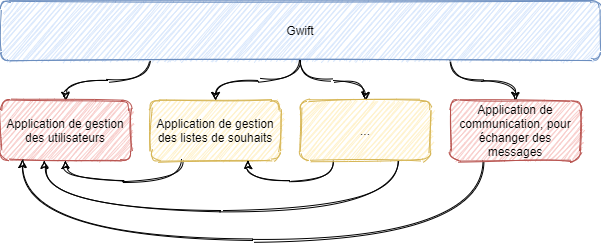
\includegraphics[width=2.5truein]{images/django/django-project-vs-apps-gwift.png}
\caption{}

\end{figure}

\hypertarget{x-besoins-utilisateurs}{\chapter{Besoins utilisateurs}}
Nous souhaitons développer un site où un utilisateur donné peut créer une liste contenant des souhaits et où d’autres utilisateurs, authentifiés ou non, peuvent choisir les souhaits à la réalisation desquels ils souhaitent participer.


Il sera nécessaire de s’authentifier pour :


\begin{itemize}

\item Créer une liste associée à l’utilisateur en cours

\item Ajouter un nouvel élément à une liste

\end{itemize}


Il ne sera pas nécessaire de s’authentifier pour :


\begin{itemize}

\item Faire une promesse d’offre pour un élément appartenant à une liste, associée à un utilisateur.

\end{itemize}


L’utilisateur ayant créé une liste pourra envoyer un email directement depuis le site aux personnes avec qui il souhaite partager sa liste, cet email contenant un lien permettant d’accéder à cette liste.


A chaque souhait, on pourrait de manière facultative ajouter un prix. Dans ce cas, le souhait pourrait aussi être subdivisé en plusieurs parties, de manière à ce que plusieurs personnes puissent participer à sa réalisation.


Un souhait pourrait aussi être réalisé plusieurs fois. Ceci revient à dupliquer le souhait en question.


\hypertarget{x-besoins-fonctionnels}{\chapter{Besoins fonctionnels}}
\hypertarget{x-gestion-des-utilisateurs}{\section{Gestion des utilisateurs}}
Pour gérer les utilisateurs, nous allons faire en sorte de surcharger ce que Django propose: par défaut, on a une la possibilité de gérer des utilisateurs (identifiés par une adresse email, un nom, un prénom, …​) mais sans plus.


Ce qu’on peut souhaiter, c’est que l’utilisateur puisse s’authentifier grâce à une plateforme connue (Facebook, Twitter, Google, etc.), et qu’il puisse un minimum gérer son profil.


\hypertarget{x-gestion-des-listes}{\section{Gestion des listes}}
\hypertarget{x-modèlisation}{\subsection{Modèlisation}}
Les données suivantes doivent être associées à une liste:


\begin{itemize}

\item un identifiant

\item un identifiant externe (un GUID, par exemple)

\item un nom

\item une description

\item le propriétaire, associé à l’utilisateur qui l’aura créée

\item une date de création

\item une date de modification

\end{itemize}


\hypertarget{x-fonctionnalités}{\subsection{Fonctionnalités}}
\begin{itemize}

\item Un utilisateur authentifié doit pouvoir créer, modifier, désactiver et supprimer une liste dont il est le propriétaire

\item Un utilisateur doit pouvoir associer ou retirer des souhaits à une liste dont il est le propriétaire

\item Il faut pouvoir accéder à une liste, avec un utilisateur authentifier ou non, \textbf{via} son identifiant externe

\item Il faut pouvoir envoyer un email avec le lien vers la liste, contenant son identifiant externe

\item L’utilisateur doit pouvoir voir toutes les listes qui lui appartiennent

\end{itemize}


\hypertarget{x-gestion-des-souhaits}{\section{Gestion des souhaits}}
\hypertarget{x-modélisation}{\subsection{Modélisation}}
Les données suivantes peuvent être associées à un souhait:


\begin{itemize}

\item un identifiant

\item identifiant de la liste

\item un nom

\item une description

\item le propriétaire

\item une date de création

\item une date de modification

\item une image, afin de représenter l’objet ou l’idée

\item un nombre (1 par défaut)

\item un prix facultatif

\item un nombre de part, facultatif également, si un prix est fourni.

\end{itemize}


\hypertarget{x-fonctionnalités}{\subsection{Fonctionnalités}}
\begin{itemize}

\item Un utilisateur authentifié doit pouvoir créer, modifier, désactiver et supprimer un souhait dont il est le propriétaire.

\item On ne peut créer un souhait sans liste associée

\item Il faut pouvoir fractionner un souhait uniquement si un prix est donné.

\item Il faut pouvoir accéder à un souhait, avec un utilisateur authentifié ou non.

\item Il faut pouvoir réaliser un souhait ou une partie seulement, avec un utilisateur authentifié ou non.

\item Un souhait en cours de réalisation et composé de différentes parts ne peut plus être modifié.

\item Un souhait en cours de réalisation ou réalisé ne peut plus être supprimé.

\item On peut modifier le nombre de fois qu’un souhait doit être réalisé dans la limite des réalisations déjà effectuées.

\end{itemize}


\hypertarget{x-gestion-des-réalisations-de-souhaits}{\section{Gestion des réalisations de souhaits}}
\hypertarget{x-modélisation}{\subsection{Modélisation}}
Les données suivantes peuvent être associées à une réalisation de souhait:


\begin{itemize}

\item identifiant du souhait

\item identifiant de l’utilisateur si connu

\item identifiant de la personne si utilisateur non connu

\item un commentaire

\item une date de réalisation

\end{itemize}


\hypertarget{x-fonctionnalités}{\subsection{Fonctionnalités}}
\begin{itemize}

\item L’utilisateur doit pouvoir voir si un souhait est réalisé, en partie ou non. Il doit également avoir un pourcentage de complétion sur la possibilité de réalisation de son souhait, entre 0% et 100%.

\item L’utilisateur doit pouvoir voir la ou les personnes ayant réalisé un souhait.

\item Il y a autant de réalisation que de parts de souhait réalisées ou de nombre de fois que le souhait est réalisé.

\end{itemize}


\hypertarget{x-gestion-des-personnes-réalisants-les-souhaits-et-qui-ne-sont-pas-connues}{\section{Gestion des personnes réalisants les souhaits et qui ne sont pas connues}}
\hypertarget{x-modélisation}{\subsection{Modélisation}}
Les données suivantes peuvent être associées à une personne réalisant un souhait:


\begin{itemize}

\item un identifiant

\item un nom

\item une adresse email facultative

\end{itemize}


\hypertarget{x-fonctionnalités}{\subsection{Fonctionnalités}}
\begin{sidebar}
Modélisation
\end{sidebar}

L’ORM de Django permet de travailler uniquement avec une définition de classes, et de faire en sorte que le lien avec la base de données soit géré uniquement de manière indirecte, par Django lui-même. On peut schématiser ce comportement par  une classe = une table.


Comme on l’a vu dans la description des fonctionnalités, on va \textbf{grosso modo} avoir besoin des éléments suivants:


\begin{itemize}

\item Des listes de souhaits

\item Des éléments qui composent ces listes

\item Des parts pouvant composer chacun de ces éléments

\item Des utilisateurs pour gérer tout ceci.

\end{itemize}


Nous proposons dans un premier temps d’éluder la gestion des utilisateurs, et de simplement se concentrer sur les fonctionnalités principales.
Cela nous donne ceci:


\begin{enumerate}

\item{code-block:: python}

\begin{verbatim}
# wish/models.py
\end{verbatim}

\begin{verbatim}
from django.db import models
\end{verbatim}

\begin{verbatim}
class Wishlist(models.Model):
    pass
\end{verbatim}

\begin{verbatim}
class Item(models.Model):
    pass
\end{verbatim}

\begin{verbatim}
class Part(models.Model):
    pass
\end{verbatim}
\end{enumerate}


Les classes sont créées, mais vides. Entrons dans les détails.


\begin{sidebar}
Listes de souhaits
\end{sidebar}

Comme déjà décrit précédemment, les listes de souhaits peuvent s’apparenter simplement à un objet ayant un nom et une description. Pour rappel, voici ce qui avait été défini dans les spécifications:


\begin{itemize}

\item un identifiant

\item un identifiant externe

\item un nom

\item une description

\item une date de création

\item une date de modification

\end{itemize}


Notre classe \texttt{Wishlist} peut être définie de la manière suivante:


\begin{enumerate}

\item{code-block:: python}

\begin{verbatim}
# wish/models.py
\end{verbatim}

\begin{verbatim}
class Wishlist(models.Model):
\end{verbatim}

\begin{verbatim}
name = models.CharField(max_length=255)
description = models.TextField()
created_at = models.DateTimeField(auto_now_add=True)
updated_at = models.DateTimeField(auto_now=True)
external_id = models.UUIDField(unique=True, default=uuid.uuid4, editable=False)
\end{verbatim}
\end{enumerate}


Que peut-on constater?


\begin{itemize}

\item Que s’il n’est pas spécifié, un identifiant \texttt{id} sera automatiquement généré et accessible dans le modèle. Si vous souhaitez malgré tout spécifier que ce soit un champ en particulier qui devienne la clé primaire, il suffit de l’indiquer grâce à l’attribut \texttt{primary\_key=True}.

\item Que chaque type de champs (\texttt{DateTimeField}, \texttt{CharField}, \texttt{UUIDField}, etc.) a ses propres paramètres d’initialisation. Il est intéressant de les apprendre ou de se référer à la documentation en cas de doute.

\end{itemize}


Au niveau de notre modélisation:


\begin{itemize}

\item La propriété \texttt{created\_at} est gérée automatiquement par Django grâce à l’attribut \texttt{auto\_now\_add}: de cette manière, lors d’un \textbf{ajout}, une valeur par défaut ("\textbf{maintenant}") sera attribuée à cette propriété.

\item La propriété \texttt{updated\_at} est également gérée automatique, cette fois grâce à l’attribut \texttt{auto\_now} initialisé à \texttt{True}: lors d’une \textbf{mise à jour}, la propriété se verra automatiquement assigner la valeur du moment présent. Cela ne permet évidemment pas de gérer un historique complet et ne nous dira pas \textbf{quels champs} ont été modifiés, mais cela nous conviendra dans un premier temps.

\item La propriété \texttt{external\_id} est de type \texttt{UUIDField}. Lorsqu’une nouvelle instance sera instanciée, cette propriété prendra la valeur générée par la fonction \texttt{uuid.uuid4()}. \textbf{A priori}, chacun des types de champs possède une propriété \texttt{default}, qui permet d’initialiser une valeur sur une nouvelle instance.

\end{itemize}


\begin{sidebar}
Souhaits
\end{sidebar}

Nos souhaits ont besoin des propriétés suivantes:


\begin{itemize}

\item un identifiant

\item l’identifiant de la liste auquel le souhait est lié

\item un nom

\item une description

\item le propriétaire

\item une date de création

\item une date de modification

\item une image permettant de le représenter.

\item un nombre (1 par défaut)

\item un prix facultatif

\item un nombre de part facultatif, si un prix est fourni.

\end{itemize}


Après implémentation, cela ressemble à ceci:


\begin{enumerate}

\item{code-block:: python}

\begin{verbatim}
# wish/models.py
\end{verbatim}

\begin{verbatim}
class Wish(models.Model):
\end{verbatim}

\begin{verbatim}
wishlist = models.ForeignKey(Wishlist)
name = models.CharField(max_length=255)
description = models.TextField()
created_at = models.DateTimeField(auto_now_add=True)
updated_at = models.DateTimeField(auto_now=True)
picture = models.ImageField()
numbers_available = models.IntegerField(default=1)
number_of_parts = models.IntegerField(null=True)
estimated_price = models.DecimalField(max_digits=19, decimal_places=2,
                                        null=True)
\end{verbatim}
\end{enumerate}


A nouveau, que peut-on constater ?


\begin{itemize}

\item Les clés étrangères sont gérées directement dans la déclaration du modèle. Un champ de type ForeignKey  permet de déclarer une relation 1-N entre deux classes. Dans la même veine, une relation 1-1 sera représentée par un champ de type OneToOneField  alors qu’une relation N-N utilisera un ManyToManyField .

\item L’attribut \texttt{default} permet de spécifier une valeur initiale, utilisée lors de la construction de l’instance. Cet attribut peut également être une fonction.

\item Pour rendre un champ optionnel, il suffit de lui ajouter l’attribut \texttt{null=True}.

\item Comme cité ci-dessus, chaque champ possède des attributs spécifiques. Le champ \texttt{DecimalField} possède par exemple les attributs \texttt{max\_digits} et \texttt{decimal\_places}, qui nous permettra de représenter une valeur comprise entre 0 et plus d’un milliard (avec deux chiffres décimaux).

\item L’ajout d’un champ de type \texttt{ImageField} nécessite l’installation de \texttt{pillow} pour la gestion des images. Nous l’ajoutons donc à nos pré-requis, dans le fichier \texttt{requirements/base.txt}.

\end{itemize}


\begin{sidebar}
Parts
\end{sidebar}

Les parts ont besoins des propriétés suivantes:


\begin{itemize}

\item un identifiant

\item identifiant du souhait

\item identifiant de l’utilisateur si connu

\item identifiant de la personne si utilisateur non connu

\item un commentaire

\item une date de réalisation

\end{itemize}


Elles constituent la dernière étape de notre modélisation et représente la réalisation d’un souhait. Il y aura autant de part d’un souhait que le nombre de souhait à réaliser fois le nombre de part.


Elles permettent à un utilisateur de participer au souhait émis par un autre utilisateur. Pour les modéliser, une part est liée d’un côté à un souhait, et d’autre part à un utilisateur. Cela nous donne ceci:


\begin{enumerate}

\item{code-block:: python}

\begin{verbatim}
from django.contrib.auth.models import User
\end{verbatim}

\begin{verbatim}
class WishPart(models.Model):
\end{verbatim}

\begin{verbatim}
wish = models.ForeignKey(Wish)
user = models.ForeignKey(User, null=True)
unknown_user = models.ForeignKey(UnknownUser, null=True)
comment = models.TextField(null=True, blank=True)
done_at = models.DateTimeField(auto_now_add=True)
\end{verbatim}
\end{enumerate}


La classe \texttt{User} référencée au début du snippet correspond à l’utilisateur qui sera connecté. Ceci est géré par Django. Lorsqu’une requête est effectuée et est transmise au serveur, cette information sera disponible grâce à l’objet \texttt{request.user}, transmis à chaque fonction ou \textbf{Class-based-view}. C’est un des avantages d’un framework tout intégré: il vient \textbf{batteries-included} et beaucoup de détails ne doivent pas être pris en compte. Pour le moment, nous nous limiterons à ceci. Par la suite, nous verrons comment améliorer la gestion des profils utilisateurs, comment y ajouter des informations et comment gérer les cas particuliers.


La classe \texttt{UnknownUser} permet de représenter un utilisateur non enregistré sur le site et est définie au point suivant.


\begin{sidebar}
Utilisateurs inconnus
\end{sidebar}

\begin{enumerate}

\item{todo:: je supprimerais pour que tous les utilisateurs soient gérés au même endroit.}

\end{enumerate}


Pour chaque réalisation d’un souhait par quelqu’un, il est nécessaire de sauver les données suivantes, même si l’utilisateur n’est pas enregistré sur le site:


\begin{itemize}

\item un identifiant

\item un nom

\item une adresse email. Cette adresse email sera unique dans notre base de données, pour ne pas créer une nouvelle occurence si un même utilisateur participe à la réalisation de plusieurs souhaits.

\end{itemize}


Ceci nous donne après implémentation:


\begin{enumerate}

\item{code-block:: python}

\begin{verbatim}
class UnkownUser(models.Model):
\end{verbatim}

\begin{verbatim}
name = models.CharField(max_length=255)
email = models.CharField(email = models.CharField(max_length=255, unique=True)
\end{verbatim}
\end{enumerate}


\hypertarget{x-tests-unitaires}{\chapter{Tests unitaires}}
\hypertarget{x-pourquoi-s’ennuyer-à-écrire-des-tests?}{\section{Pourquoi s’ennuyer à écrire des tests?}}
Traduit grossièrement depuis un article sur https://medium.com/javascript-scene/what-every-unit-test-needs-f6cd34d9836d

\begin{verbatim}
Vos tests sont la première et la meilleure ligne de défense contre les défauts de programmation. Ils sont
\end{verbatim}

\begin{verbatim}
Les tests unitaires combinent de nombreuses fonctionnalités, qui en fait une arme secrète au service d'un développement réussi:
\end{verbatim}

\begin{enumerate}

\item{Aide au design: écrire des tests avant d’écrire le code vous donnera une meilleure perspective sur le design à appliquer aux API.}

\item{Documentation (pour les développeurs): chaque description d’un test}

\item{Tester votre compréhension en tant que développeur:}

\item{Assurance qualité: des tests,
5.}

\end{enumerate}


\hypertarget{x-why-bother-with-test-discipline?}{\section{Why Bother with Test Discipline?}}
Your tests are your first and best line of defense against software defects. Your tests are more important than linting \& static analysis (which can only find a subclass of errors, not problems with your actual program logic). Tests are as important as the implementation itself (all that matters is that the code meets the requirement — how it’s implemented doesn’t matter at all unless it’s implemented poorly).


Unit tests combine many features that make them your secret weapon to application success:


\begin{enumerate}

\item{Design aid: Writing tests first gives you a clearer perspective on the ideal API design.}

\item{Feature documentation (for developers): Test descriptions enshrine in code every implemented feature requirement.}

\item{Test your developer understanding: Does the developer understand the problem enough to articulate in code all critical component requirements?}

\item{Quality Assurance: Manual QA is error prone. In my experience, it’s impossible for a developer to remember all features that need testing after making a change to refactor, add new features, or remove features.}

\item{Continuous Delivery Aid: Automated QA affords the opportunity to automatically prevent broken builds from being deployed to production.}

\end{enumerate}


Unit tests don’t need to be twisted or manipulated to serve all of those broad-ranging goals. Rather, it is in the essential nature of a unit test to satisfy all of those needs. These benefits are all side-effects of a well-written test suite with good coverage.


\hypertarget{x-what-are-you-testing?}{\section{What are you testing?}}
\begin{enumerate}

\item{What component aspect are you testing?}

\item{What should the feature do? What specific behavior requirement are you testing?}

\end{enumerate}


\hypertarget{x-couverture-de-code}{\section{Couverture de code}}
On a vu au chapitre 1 qu’il était possible d’obtenir une couverture de code, c’est-à-dire un pourcentage.


\hypertarget{x-comment-tester-?}{\section{Comment tester ?}}
Il y a deux manières d’écrire les tests: soit avant, soit après l’implémentation. Oui, idéalement, les tests doivent être écrits à l’avance. Entre nous, on ne va pas râler si vous faites l’inverse, l’important étant que vous le fassiez. Une bonne métrique pour vérifier l’avancement des tests est la couverture de code.


Pour l’exemple, nous allons écrire la fonction \texttt{percentage\_of\_completion} sur la classe \texttt{Wish}, et nous allons spécifier les résultats attendus avant même d’implémenter son contenu. Prenons le cas où nous écrivons la méthode avant son test:


\begin{verbatim}
class Wish(models.Model):

    [...]

    @property
    def percentage_of_completion(self):
        """
        Calcule le pourcentage de complétion pour un élément.
        """
        number_of_linked_parts = WishPart.objects.filter(wish=self).count()
        total = self.number_of_parts * self.numbers_available
        percentage = (number_of_linked_parts / total)
        return percentage * 100
\end{verbatim}

Lancez maintenant la couverture de code. Vous obtiendrez ceci:


\begin{verbatim}
$ coverage run --source "." src/manage.py test wish
$ coverage report

Name                             Stmts   Miss Branch BrPart  Cover
------------------------------------------------------------------
src\gwift\__init__.py                0      0      0      0   100%
src\gwift\settings\__init__.py       4      0      0      0   100%
src\gwift\settings\base.py          14      0      0      0   100%
src\gwift\settings\dev.py            8      0      2      0   100%
src\manage.py                        6      0      2      1    88%
src\wish\__init__.py                 0      0      0      0   100%
src\wish\admin.py                    1      0      0      0   100%
src\wish\models.py                  36      5      0      0    88%
------------------------------------------------------------------
TOTAL                               69      5      4      1    93%
\end{verbatim}

Si vous générez le rapport HTML avec la commande \texttt{coverage html} et que vous ouvrez le fichier \texttt{coverage\_html\_report/src\_wish\_models\_py.html}, vous verrez que les méthodes en rouge ne sont pas testées.
\textbf{A contrario}, la couverture de code atteignait \textbf{98\%} avant l’ajout de cette nouvelle méthode.


Pour cela, on va utiliser un fichier tests.py dans notre application \texttt{wish}. \textbf{A priori}, ce fichier est créé automatiquement lorsque vous initialisez une nouvelle application.


\begin{verbatim}
from django.test import TestCase

class TestWishModel(TestCase):
    def test_percentage_of_completion(self):
        """
        Vérifie que le pourcentage de complétion d'un souhait
        est correctement calculé.

        Sur base d'un souhait, on crée quatre parts et on vérifie
        que les valeurs s'étalent correctement sur 25%, 50%, 75% et 100%.
        """
        wishlist = Wishlist(name='Fake WishList',
                            description='This is a faked wishlist')
        wishlist.save()

        wish = Wish(wishlist=wishlist,
                    name='Fake Wish',
                    description='This is a faked wish',
                    number_of_parts=4)
        wish.save()

        part1 = WishPart(wish=wish, comment='part1')
        part1.save()
        self.assertEqual(25, wish.percentage_of_completion)

        part2 = WishPart(wish=wish, comment='part2')
        part2.save()
        self.assertEqual(50, wish.percentage_of_completion)

        part3 = WishPart(wish=wish, comment='part3')
        part3.save()
        self.assertEqual(75, wish.percentage_of_completion)

        part4 = WishPart(wish=wish, comment='part4')
        part4.save()
        self.assertEqual(100, wish.percentage_of_completion)
\end{verbatim}

L’attribut \texttt{property} sur la méthode \texttt{percentage\_of\_completion()} va nous permettre d’appeler directement la méthode \texttt{percentage\_of\_completion()} comme s’il s’agissait d’une propriété de la classe, au même titre que les champs \texttt{number\_of\_parts} ou \texttt{numbers\_available}. Attention que ce type de méthode contactera la base de données à chaque fois qu’elle sera appelée. Il convient de ne pas surcharger ces méthodes de connexions à la base: sur de petites applications, ce type de comportement a très peu d’impacts, mais ce n’est plus le cas sur de grosses applications ou sur des méthodes fréquemment appelées. Il convient alors de passer par un mécanisme de \textbf{cache}, que nous aborderons plus loin.


En relançant la couverture de code, on voit à présent que nous arrivons à 99%:


\begin{verbatim}
$ coverage run --source='.' src/manage.py test wish; coverage report; coverage html;
.
----------------------------------------------------------------------
Ran 1 test in 0.006s

OK
Creating test database for alias 'default'...
Destroying test database for alias 'default'...
Name                             Stmts   Miss Branch BrPart  Cover
------------------------------------------------------------------
src\gwift\__init__.py                0      0      0      0   100%
src\gwift\settings\__init__.py       4      0      0      0   100%
src\gwift\settings\base.py          14      0      0      0   100%
src\gwift\settings\dev.py            8      0      2      0   100%
src\manage.py                        6      0      2      1    88%
src\wish\__init__.py                 0      0      0      0   100%
src\wish\admin.py                    1      0      0      0   100%
src\wish\models.py                  34      0      0      0   100%
src\wish\tests.py                   20      0      0      0   100%
------------------------------------------------------------------
TOTAL                               87      0      4      1    99%
\end{verbatim}

En continuant de cette manière (ie. Ecriture du code et des tests, vérification de la couverture de code), on se fixe un objectif idéal dès le début du projet. En prenant un développement en cours de route, fixez-vous comme objectif de ne jamais faire baisser la couverture de code.


\hypertarget{x-quelques-liens-utiles}{\section{Quelques liens utiles}}
\begin{itemize}

\item Django factory boy 

\end{itemize}


\hypertarget{x-refactoring}{\chapter{Refactoring}}
On constate que plusieurs classes possèdent les mêmes propriétés \texttt{created\_at} et \texttt{updated\_at}, initialisées aux mêmes valeurs. Pour gagner en cohérence, nous allons créer une classe dans laquelle nous définirons ces deux champs, et nous ferons en sorte que les classes \texttt{Wishlist}, \texttt{Item} et \texttt{Part} en héritent. Django gère trois sortes d’héritage:


\begin{itemize}

\item L’héritage par classe abstraite

\item L’héritage classique

\item L’héritage par classe proxy.

\end{itemize}


\hypertarget{x-classe-abstraite}{\section{Classe abstraite}}
L’héritage par classe abstraite consiste à déterminer une classe mère qui ne sera jamais instanciée. C’est utile pour définir des champs qui se répèteront dans plusieurs autres classes et surtout pour respecter le principe de DRY. Comme la classe mère ne sera jamais instanciée, ces champs seront en fait dupliqués physiquement, et traduits en SQL, dans chacune des classes filles.


\begin{verbatim}
# wish/models.py

class AbstractModel(models.Model):
    class Meta:
        abstract = True

    created_at = models.DateTimeField(auto_now_add=True)
    updated_at = models.DateTimeField(auto_now=True)


class Wishlist(AbstractModel):
    pass


class Item(AbstractModel):
    pass


class Part(AbstractModel):
    pass
\end{verbatim}

En traduisant ceci en SQL, on aura en fait trois tables, chacune reprenant les champs \texttt{created\_at} et \texttt{updated\_at}, ainsi que son propre identifiant:


\begin{verbatim}
--$ python manage.py sql wish
BEGIN;
CREATE TABLE "wish_wishlist" (
    "id" integer NOT NULL PRIMARY KEY AUTOINCREMENT,
    "created_at" datetime NOT NULL,
    "updated_at" datetime NOT NULL
)
;
CREATE TABLE "wish_item" (
    "id" integer NOT NULL PRIMARY KEY AUTOINCREMENT,
    "created_at" datetime NOT NULL,
    "updated_at" datetime NOT NULL
)
;
CREATE TABLE "wish_part" (
    "id" integer NOT NULL PRIMARY KEY AUTOINCREMENT,
    "created_at" datetime NOT NULL,
    "updated_at" datetime NOT NULL
)
;

COMMIT;
\end{verbatim}

\hypertarget{x-héritage-classique}{\section{Héritage classique}}
L’héritage classique est généralement déconseillé, car il peut introduire très rapidement un problème de performances: en reprenant l’exemple introduit avec l’héritage par classe abstraite, et en omettant l’attribut \texttt{abstract = True}, on se retrouvera en fait avec quatre tables SQL:


\begin{itemize}

\item Une table \texttt{AbstractModel}, qui reprend les deux champs \texttt{created\_at} et \texttt{updated\_at}

\item Une table \texttt{Wishlist}

\item Une table \texttt{Item}

\item Une table \texttt{Part}.

\end{itemize}


A nouveau, en analysant la sortie SQL de cette modélisation, on obtient ceci:


\begin{verbatim}
--$ python manage.py sql wish

BEGIN;
CREATE TABLE "wish_abstractmodel" (
    "id" integer NOT NULL PRIMARY KEY AUTOINCREMENT,
    "created_at" datetime NOT NULL,
    "updated_at" datetime NOT NULL
)
;
CREATE TABLE "wish_wishlist" (
    "abstractmodel_ptr_id" integer NOT NULL PRIMARY KEY REFERENCES "wish_abstractmodel" ("id")
)
;
CREATE TABLE "wish_item" (
    "abstractmodel_ptr_id" integer NOT NULL PRIMARY KEY REFERENCES "wish_abstractmodel" ("id")
)
;
CREATE TABLE "wish_part" (
    "abstractmodel_ptr_id" integer NOT NULL PRIMARY KEY REFERENCES "wish_abstractmodel" ("id")
)
;

COMMIT;
\end{verbatim}

Le problème est que les identifiants seront définis et incrémentés au niveau de la table mère. Pour obtenir les informations héritées, nous seront obligés de faire une jointure. En gros, impossible d’obtenir les données complètes pour l’une des classes de notre travail de base sans effectuer un \textbf{join} sur la classe mère.


Dans ce sens, cela va encore…​ Mais imaginez que vous définissiez une classe \texttt{Wishlist}, de laquelle héritent les classes \texttt{ChristmasWishlist} et \texttt{EasterWishlist}: pour obtenir la liste complètes des listes de souhaits, il vous faudra faire une jointure \textbf{externe} sur chacune des tables possibles, avant même d’avoir commencé à remplir vos données. Il est parfois nécessaire de passer par cette modélisation, mais en étant conscient des risques inhérents.


\hypertarget{x-classe-proxy}{\section{Classe proxy}}
Lorsqu’on définit une classe de type \textbf{proxy}, on fait en sorte que cette nouvelle classe ne définisse aucun nouveau champ sur la classe mère. Cela ne change dès lors rien à la traduction du modèle de données en SQL, puisque la classe mère sera traduite par une table, et la classe fille ira récupérer les mêmes informations dans la même table: elle ne fera qu’ajouter ou modifier un comportement dynamiquement, sans ajouter d’emplacements de stockage supplémentaires.


Nous pourrions ainsi définir les classes suivantes:


\begin{verbatim}
# wish/models.py

class Wishlist(models.Model):
    name = models.CharField(max_length=255)
    description = models.CharField(max_length=2000)
    expiration_date = models.DateField()

    @staticmethod
    def create(self, name, description, expiration_date=None):
        wishlist = Wishlist()
        wishlist.name = name
        wishlist.description = description
        wishlist.expiration_date = expiration_date
        wishlist.save()
        return wishlist

class ChristmasWishlist(Wishlist):
    class Meta:
        proxy = True

    @staticmethod
    def create(self, name, description):
        christmas = datetime(current_year, 12, 31)
        w = Wishlist.create(name, description, christmas)
        w.save()


class EasterWishlist(Wishlist):
    class Meta:
        proxy = True

    @staticmethod
    def create(self, name, description):
        expiration_date = datetime(current_year, 4, 1)
        w = Wishlist.create(name, description, expiration_date)
        w.save()
\end{verbatim}

\begin{sidebar}
Gestion des utilisateurs
\end{sidebar}

Dans les spécifications, nous souhaitions pouvoir associer un utilisateur à une liste (\textbf{le propriétaire}) et un utilisateur à une part (\textbf{le donateur}). Par défaut, Django offre une gestion simplifiée des utilisateurs (pas de connexion LDAP, pas de double authentification, …​): juste un utilisateur et un mot de passe. Pour y accéder, un paramètre par défaut est défini dans votre fichier de settings: \texttt{AUTH\_USER\_MODEL}.


\hypertarget{x-khana}{\chapter{Khana}}
Khana est une application de suivi d’apprentissage pour des élèves ou étudiants.
Nous voulons pouvoir:


\begin{enumerate}

\item{Lister les élèves}

\item{Faire des listes de présence pour les élèves}

\item{Pouvoir planifier ses cours}

\item{Pouvoir suivre l’apprentissage des élèves, les liens qu’ils ont entre les éléments à apprendre:}

\item{pour écrire une phrase, il faut pouvoir écrire des mots, connaître la grammaire, et connaître la conjugaison}

\item{pour écrire des mots, il faut savoir écrire des lettres}

\item{…​}

\end{enumerate}


Plusieurs professeurs s’occupent d’une même classe; il faut pouvoir écrire des notes, envoyer des messages aux autres professeurs, etc.


Il faut également pouvoir définir des dates de contrôle, voir combien de semaines il reste pour s’assurer d’avoir vu toute la matiètre.


Et pouvoir encoder les points des contrôles.


\begin{figure}[h]{}
\centering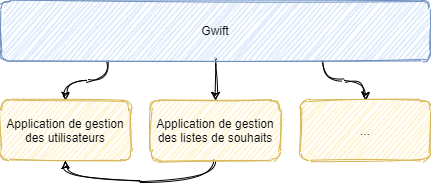
\includegraphics[width=2.5truein]{images/django/django-project-vs-apps-khana.png}
\caption{}

\end{figure}

\hypertarget{x-ressources-et-bibliographie}{\part*{Ressources et bibliographie}}
\begin{itemize}

\item \href{https://simpleisbetterthancomplex.com/series/beginners-guide/1.11/}{Simple Is Better Than Complex}

\item \href{https://www.feldroy.com/collections/two-scoops-press/products/two-scoops-of-django-1-11}{Two Scoops of Django 1.11}

\item \href{https://www.feldroy.com/products/django-crash-course}{Django Crash Course}

\item \href{https://www.amazon.com/dp/B07BDGC57}{Django Design Patterns and Best Practices} (Packt Publishing)

\item \href{https://books.agiliq.com/en/latest/README.html}{Books by Agiliq}

\end{itemize}


\hypertarget{x-snippets-utiles-(et-forcément-dispensables)}{\chapter{Snippets utiles (et forcément dispensables)}}
\hypertarget{x-récupération-du-dernier-tag-git-en-python}{\section{Récupération du dernier tag Git en Python}}
L’idée ici est simplement de pouvoir afficher le numéro de version ou le hash d’exécution du code, sans avoir à se connecter au dépôt. Cela apporte une certaine transparence, \textbf{sous réserve que le code soit géré par Git}. Si vous suivez scrupuleusement les 12 facteurs, la version de l’application déployée n’est plus sensée conserver un lien avec votre dépôt d’origine…​ Si vous déployez votre code en utilisant un \texttt{git fetch} puis un \texttt{git checkout <tag\_name>}, le morceau de code ci-dessous pourra vous intéresser :-)


\begin{verbatim}

\end{verbatim}

\hypertarget{x-applications-\emph{legacy}}{\chapter{Applications \emph{Legacy}}}
Quand on intègre une nouvelle application Django dans un environement existant, la première étape est de se câbler sur la base de données existantes;


\begin{enumerate}

\item{Soit l’application sur laquelle on se greffe restera telle quelle;}

\item{Soit l’application est \textbf{remplacée} par la nouvelle application Django.}

\begin{verbatim}
Dans le premier cas, il convient de créer une application et de spécifier pour chaque classe l'attribute `managed = False` dans le `class Meta:` de la définition.
Dans le second, il va falloir câbler deux-trois éléments avant d'avoir une intégration complète (comprendre: avec une interface d'admin, les migrations, les tests unitaires et tout le brol :))
\end{verbatim}

\begin{verbatim}
`python manage.py inspectdb > models.py`
\end{verbatim}

\begin{enumerate}

\item{\href{https://simpleisbetterthancomplex.com/series/beginners-guide/1.11/}{A Complete Beginner’s Guide to Django}:}

\item{\href{https://simpleisbetterthancomplex.com/series/2017/09/04/a-complete-beginners-guide-to-django-part-1.html}{Getting Started}}

\item{\href{https://simpleisbetterthancomplex.com/series/2017/09/11/a-complete-beginners-guide-to-django-part-2.html}{Fundamentals}}

\item{\href{https://simpleisbetterthancomplex.com/series/2017/09/18/a-complete-beginners-guide-to-django-part-3.html}{Advanced Concepts}}

\item{\href{https://simpleisbetterthancomplex.com/series/2017/09/25/a-complete-beginners-guide-to-django-part-4.html}{Authentication}}

\item{\href{https://simpleisbetterthancomplex.com/series/2017/10/02/a-complete-beginners-guide-to-django-part-5.html}{Django ORM}}

\item{\href{https://simpleisbetterthancomplex.com/series/2017/10/09/a-complete-beginners-guide-to-django-part-6.html}{Class Based Views}}

\item{\href{https://simpleisbetterthancomplex.com/series/2017/10/16/a-complete-beginners-guide-to-django-part-7.html}{Deployment}}

\end{enumerate}

\end{enumerate}


\hypertarget{x-livres}{\chapter{Livres}}
\begin{itemize}

\item \href{https://www.packtpub.com/product/expert-python-programming-third-edition/9781789808896}{Expert Python Programming - Third Edition} - pour les chapitres sur Docker, Vagrant.

\end{itemize}


\end{document}

